\documentclass[12pt, notitlepage]{report}
\usepackage{graphicx} % embed graphics
\usepackage[margin=0.5in, top=1in, bottom=1in]{geometry}
\usepackage{titlesec} % custom headings
\usepackage{hyperref} % clickable contents
\usepackage{fancyhdr} % custom header/footer
\usepackage{float}
\usepackage{pdfpages} % so we can add schematics
\usepackage[nonumberlist,acronym,toc,numberedsection=autolabel]{glossaries} % for the acronyms
\usepackage{tabularx} % table macros
\usepackage{dirtree}
\usepackage{amsmath}

\usepackage{framed,color,verbatim}
\definecolor{shadecolor}{rgb}{.9, .9, .9}
\newenvironment{code}%
   {\snugshade\verbatim}%
   {\endverbatim\endsnugshade}

\setlength{\headheight}{15pt}
\titleformat{\chapter}{\Huge\bfseries}{\thechapter}{0.5em}{}
\titlespacing{\chapter}{0in}{-0.3in}{0.2in}
\let\oldch\chapter
\renewcommand{\chapter}{\clearpage\oldch}
%\titlespacing{\section}{0in}{0in}{0.3in}

\pagestyle{fancy}
\fancyhf{}
\lhead{Sun Devil Motorsports}
\rhead{SDM-23 DAQ Design Report}
\cfoot{\thepage}
\fancypagestyle{plain}{
    \fancyhf{}
\lhead{Sun Devil Motorsports}
\rhead{SDM-23 DAQ Design Report}
\cfoot{\thepage}
}


\newcommand\setrow[1]{\gdef\rowmac{#1}#1\ignorespaces}
\newcommand\clearrow{\global\let\rowmac\relax}
\clearrow



%\pagenumbering{roman}
\makeglossaries


\begin{document}

\begin{titlepage}
    \centering
    \vfill
    \textbf{\Huge SDM-23 Data Acquisition}\vspace{1em}\\
    \textbf{\Large Design Report}
    \vfill
    
\includegraphics[width=7.5in]{images/logo.png}
    \vfill
    \textbf{2023 Formula SAE Design Report}\\
    \textbf{Arizona State University}\\
    \vspace{1em}
    Authors\\
        Joshua Tenorio\\
        Ryan Leigh\\
        Tolemy Nibi
    \vfill
    \centering
\includegraphics[width=2.5in]{images/seal.png}
    \vfill
\end{titlepage}
\stepcounter{page}
\tableofcontents
\pagebreak
\begin{abstract}
    \thispagestyle{plain}
    \addcontentsline{toc}{chapter}{Abstract}
The SDM-23 Data Acquisition (DAQ) package provides data logging and analysis capabilities for SDM-23, Sun Devil Motorsports' challenger for the Formula SAE Michigan 2023 ICE Competition.
It was designed and implemented over the course of the 2022-23 school year.
\vspace{1em}

The package includes (but is not limited to) capabilities to measure and log longitudinal and lateral acceleration, brake pressure and rotor temperature, steering wheel angle, and GPS location of the car.
The data collected can be used to validate the team's designs and provide feedback for drivers and future designs.
\vspace{1em}

This report details the goals, design, and implementation of the DAQ package, as well as the results of implementation and testing and recommendations for future work.
\end{abstract}

\chapter{Introduction}
Formula SAE is a collegiate engineering design competition where teams are tasked to design, manufacture, and compete with an Formula-style race car each year.
Teams are judged on the business aspect, the design aspect, and the performance aspect of their car.
An integral part of the design and performance aspect is real-world validation, for justifying and validating design choices as well as quantifying what changes to the car can provide the best performance.
\begin{figure}[H]
    \centering
    \includegraphics[width=5in]{images/sdm23-unveil.JPG}
    \caption{SDM-23 during unveil testing at Podium Club in Attesa}
    \label{fig:sdm23-unveil}
\end{figure}

The Data Acquisition subteam of Sun Devil Motorsports, Arizona State's Formula SAE team, is responsible for producing a DAQ package that can reliably collect data.
This report will detail the design and implementation of the DAQ package for SDM-23, Sun Devil Motorsports' 2022-23 car, as well as results of implementation and testing and recommendations for future work.
\vspace{1em}

A DAQ package can be broken up into a few high-level components:
\begin{itemize}
    \item Sensors which respond to physical stimuli and either transmit signals or change electrical property (e.g., resistance)
    \item A data logger that can measure electrical signals from sensors, convert it into a useful measurement, and store it in memory
    \item Software, typically on a PC, that can retrieve and process data from the data logger
\end{itemize}
The first two components make up the DAQ electrical system.
The third comes into use when retrieving and processing data from the electrical system.
\section{Project Goals}
The goals for SDM-23's Data Acquisition package are to:
\begin{itemize}
    \item Build upon SDM-22's DAQ package concept
    \item Provide consistent and useful data
    \item Increase the reliability and professionalism of DAQ wiring
\end{itemize}

\section{Project Requirements}
The following are the project requirements for the Data Acquisition package.
System-level requirements were determined by the DAQ subteam, and sensor requirements and priorities were given by other subteam leads.
\begin{enumerate}
    \item System-Level Requirements
    \begin{enumerate}
        \item The DAQ package must be standalone; the car's operation shall not need to depend on the functionality of any DAQ component.
        \item The DAQ electrical system shall be powered off of 12V from the ECU.
        \item The DAQ electrical system shall allow for expansion, i.e. additional sensors or modules can be plugged into it without major changes.
        \item Data retrieval shall be able to be accomplished by plugging a computer into the system using USB.
        \item Any communication between microcontrollers on the car shall use CAN.
    \end{enumerate}
    \item Sensor Requirements
    \begin{enumerate}
        \item Aerodynamics
        \begin{enumerate}
            \item Strain gauges on push/pull rods
            \item air speed measurements
        \end{enumerate}
        \item Brakes
        \begin{enumerate}
            \item Brake pressure
            \item Brake rotor temperature
            \item Brake fluid temperature
        \end{enumerate}
        \item Drivetrain
        \begin{enumerate}
            \item Strain gauges on drivetrain components
        \end{enumerate}
        \item Suspension
        \begin{enumerate}
            \item 3 axis gyroscope and accelerometer
            \item Multiple accelerometers
            \item Linear potentiometers
        \end{enumerate}
        \item Systems
        \begin{enumerate}
            \item Steering wheel angle
            \item Steering wheel force
        \end{enumerate}
    \end{enumerate}
\end{enumerate}



\chapter{Background}
The purpose of this chapter is to explain concepts and sensors referenced later in the report, and to describe the functionality of the sensors and hardware used in the DAQ package.
An overview of SDM-22's DAQ package has also been included for reference.
\section{Previous Design}
The DAQ package for SDM-22 was a complete overhaul of previous DAQ packages designed and manufactured by the team.
The SDM-22 DAQ package's goal was to create a permanent DAQ presence on the vehicle.
For instance this included permanent mounting spots in the vehicle for DAQ boxes.
Additionally printed circuit boards were designed for the first time to simplify wiring within each box.
A Teensy 4.1 microcontroller replaced the Arduino Mega as the main board, due to its smaller form factor, additional hardware features such as CAN and more Serial and I2C ports, as well as the built in micro SD card socket.
Teensy 4.0 microcontrollers were used for auxiliary data hubs, whose purpose were to collect data from local sensors and transmit them back to the main board.
\vspace{1em}

Although the SDM-22 DAQ package made big improvements to previous iterations, it was not without faults.
The wire connectors used in the package were difficult to use, and the system was not able to retrieve CAN data from the ECU, possibly due to a faulty CAN transceiver board.
Serial communication between the main board and data hubs were also slow at around 8 packets transmitted per second, likely due to needlessly large data packets.
Additionally, the planning and designs of the mounting solutions for the boxes were held back by the electrical design, resulting in a non-optimal mounting place for the main board.

\section{Selected Components}
The components discussed in this section are the sensors and other hardware that have been included in the DAQ package for SDM-23.

\subsection{Primary Microcontroller}
The DAQ package requires sensor processing and communication standards to reliably collect and log data from the vehicle.
The Teensy 4.1 in Figure \ref{fig:t41} is an ARM Cortex-M7 based development board with an NXP iMXRT1062 chip operating at 600 MHz.
Notably it comes with a built-in micro SD socket, 3 CAN controllers, 3 I2C and 8 Serial ports and 18 analog input pins among many other features.
This makes it a great option to use as the main data logger.
\begin{figure}[H]
        \centering
        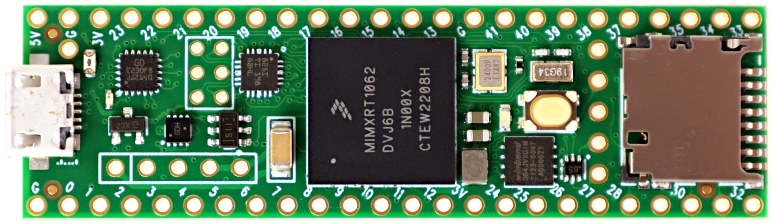
\includegraphics[width=4in]{images/teensy41.jpg}
        \caption{Teensy 4.1 Microcontroller}
        \label{fig:t41}
\end{figure}

\subsection{Auxiliary Microcontroller}
The Teensy 4.0 (Figure \ref{fig:t40}) has the same processing specs as the Teensy 4.1, but in a smaller form factor.
As such, there is less accessible GPIO pins available and no built-in SD socket.
With that said, it still has 7 Serial and 3 I2C ports, 3 CAN controllers, and 14 analog input pins, though some are not as accessible.
\vspace{1em}

%Its smaller form factor makes it a good choice for smaller data hubs that can be placed around the car.
\begin{figure}[H]
\centering
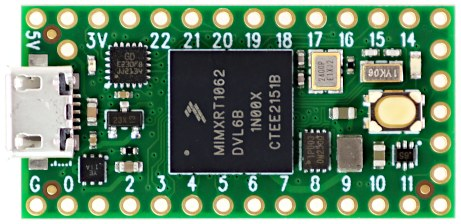
\includegraphics[width=2.2in]{images/teensy40.jpg}
\caption{Teensy 4.0 Microcontroller}
\label{fig:t40}
\end{figure}
\subsection{CAN Transceiver}
To collect data from multiple points on the car into a central location, a robust communication protocol must be implemented.
One such protocol is a Controller Area Network (CAN) bus, which is a standard in the automotive industry designed to allow devices to communicate with each other without a host system.
Devices are connected to each other via a CAN high and CAN low cable, and the network is terminated on both ends by a $120\Omega$ resistor to reduce reflections in the signal.
Each message frame has an ID to determine its priority on the bus.

\begin{figure}[H]
        \centering
        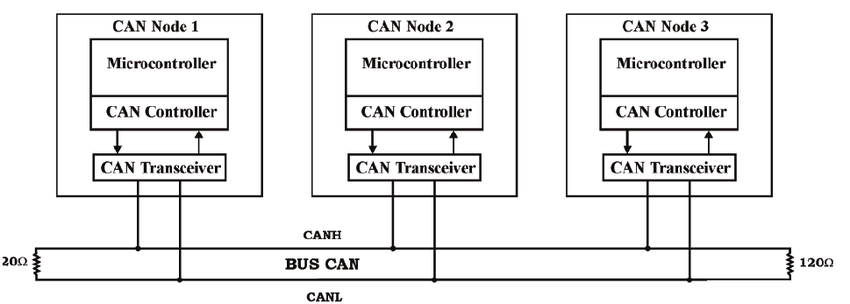
\includegraphics[width=5in]{images/iso11898-can.png}
        \caption{Diagram of a CAN bus}
        \label{fig:can-diagram}
\end{figure}
Both the Teensy 4.0 and 4.1 have a CAN controller in their chip, so to complete the CAN node only a CAN transceiver is needed for each board. This converts the data streams from the CANH and CANL to levels that the CAN controller can use. When transmitting messages the transceiver converts data streams from the controller to the CAN bus levels.
\vspace{1em}

The transceiver chosen is Texas Instruments' SN65HVD230.
It was chosen because it operated on a 3.3V level and would be able to process data from the CAN bus at 1 Mbps, which is the speed at which the Haltech ECU operates at.
This will be used to communicate with the Haltech ECU as well as within the DAQ package.
\begin{figure}[H]
        \centering
        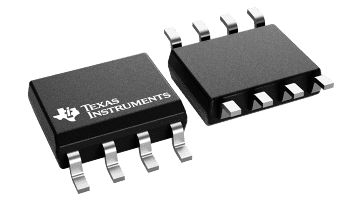
\includegraphics[width=2in]{images/sn65hvd230chip.png}
        \caption{SN65HVD230 CAN Transceiver}
        \label{fig:sn65hvd230}
\end{figure}

\subsection{Linear Potentiometer}
Potentiometers are three-terminal resistors with a sliding or rotating contact that form an adjustable voltage divider.
Linear potentiometers are mounted to SDM-23's suspension in order to measure the damper travel.
Some applications of this data include calculating damper speed and estimating downforce.
\vspace{1em}

The SparkFun X-Large Slide Pot was chosen, primarily because the team already has many in stock and prior success with it.
Although we considered purchasing new linear potentiometers such as the one offered by FSAEparts.com or Haltech, we opted against it as purchasing four of these would be expensive and irresponsible given the other needs of the data acquisition budget.
\begin{figure}[H]
        \centering
        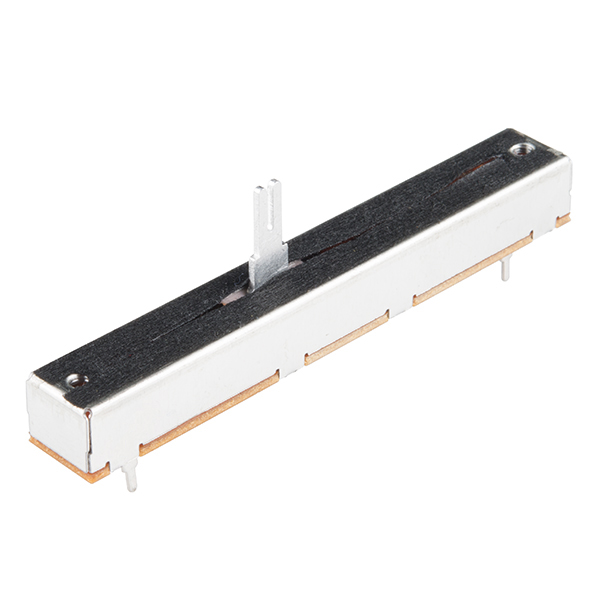
\includegraphics[width=2in]{images/slidepot.jpg}
        \caption{SparkFun X-Large Slide Pot}
        \label{fig:slidepot}
\end{figure}

\subsection{Rotary Potentiometer}
A rotary potentiometer is attached at the pinion gear of the steering rack to measure the steering wheel angle.
A 360-degree rotation potentiometer from CTS was chosen, as we did not want to deal with any interference between the steering wheel rotation and a potentiometer's hard stop.
\begin{figure}[H]
        \centering
        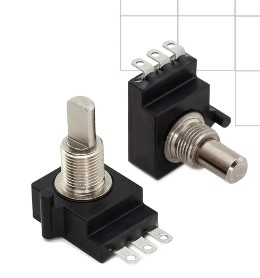
\includegraphics[width=2in]{images/pot.jpg}
        \caption{CTS Rotary Potentiometer}
        \label{fig:pot}
\end{figure}
Other options for measuring rotation include an encoder or a hall effect absolute position sensor.
Encoders are not as viable because of their reduced resolution when compared to a potentiometer, and a hall-effect based position sensor was not chosen as the team has not used them before and mounting it would be much more difficult.
\subsection{6 DoF IMU}
A 6 DoF Inertial Measurement Unit (IMU) is used to measure SDM-23's acceleration and angular velocity on 3 axes.
The module used is ST's ISM330DHCX, which is a high-performance 3D digital accelerometer and gyroscope in a single package.

The SparkFun Breakout board is used and pictured in Figure \ref{fig:ism330dhcx}.
\begin{figure}[H]
        \centering
        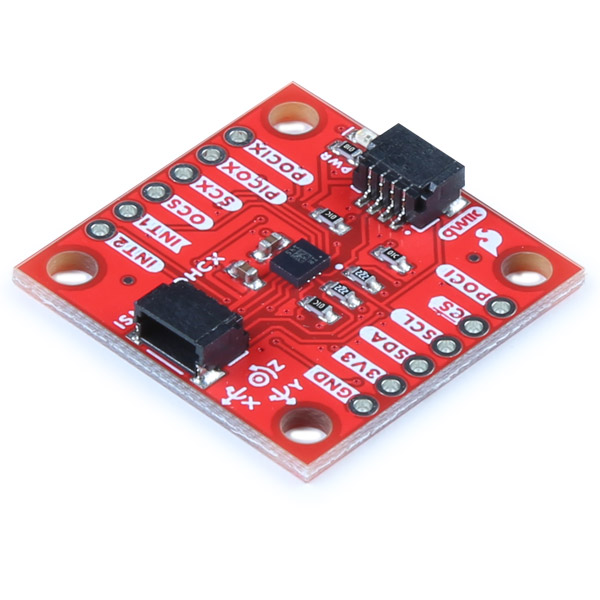
\includegraphics[width=2in]{images/6DoFIMU_03a.jpg}
        \caption{SparkFun ISM330DHCX Breakout Board}
        \label{fig:ism330dhcx}
\end{figure}
Since the Suspension subteam is interested in angular position, the angular velocity data must be integrated to produce position data.

\subsection{Infrared Temperature Sensor}
A MLX90614, an infrared thermometer, is used to measure the rotors' temperatures.
It is an I2C device that operates on 3.3V and can measure an object's temperature up to $380^\circ$C.
Additionally, we are also able to set the emissivity of the object whose temperature we are measuring.
\begin{figure}[H]
        \centering
        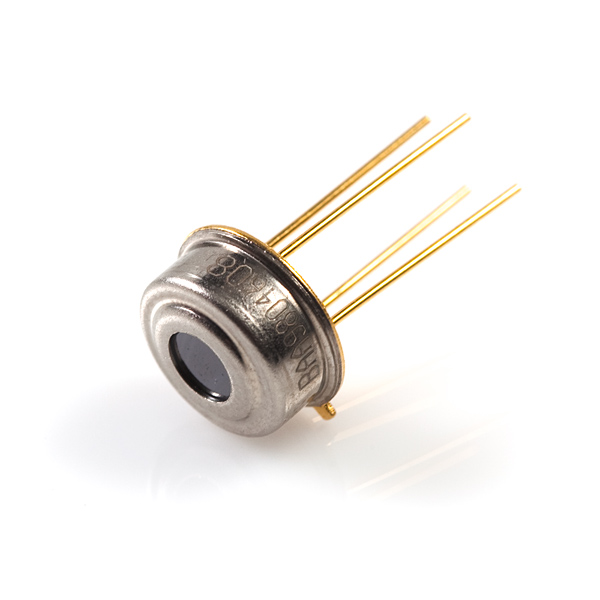
\includegraphics[width=2in]{images/mlx90614.jpg}
        \caption{MLX90614 IR Thermometer}
        \label{fig:mlx90614}
\end{figure}
One downside to infrared sensors is that they are susceptible to sunlight.
Despite this, infrared temperature sensors are still reliable for measuring brake rotor temperatures.


\subsection{Strain Gauge}
Strain gauges are attached to the push and pull rods of SDM-23's suspension.
They are able to measure strain. Using the relationship between strain and stress we can measure the loads that the push and pull rods are subject to.
\begin{figure}[H]
        \centering
        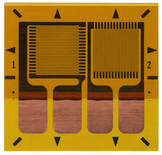
\includegraphics[width=2in]{images/Strain Gauge/125UTA.png}
        \caption{Tee Rosettes Strain Gauge: 125UTA}
        \label{fig:Tee Rosette Strain Gauge: 125UTA}
\end{figure}

Electrically, strain gauges are resistors whose resistance changes based on how they deform.
This resistance change can be measured by a Wheatstone bridge.
\vspace{1em}

Tee rosettes from Micro Measurements were chosen, because its pattern allows us to compensate for temperature without bonding an additional strain gauge, helping us save cost. Shown below are the governing equations. Where G is Shear modulus, E is Young's modulus, $\nu$ is Poisson's Ratio, $\varepsilon$ is strain, $\sigma$ is stress, $\gamma$ is shear strain, and $\tau$ is shear stress. 
\vspace{1em}

\begin{center} 
$[\sigma]_{xyz} = \begin{bmatrix}
\sigma_{xx} & \sigma_{xy}  & \sigma_{xz} \\
\sigma_{yx} & \sigma_{yy}  & \sigma_{yz} \\
\sigma_{xz} & \sigma_{yz}  & \sigma_{zz} 
\end{bmatrix}$ = 
$\begin{bmatrix} \sigma_{xx} & \tau_{xy}  & \tau_{xz} \\
\tau_{yx} & \sigma_{yy}  & \tau_{yz} \\
\tau_{xz} & \tau_{yz}  & \sigma_{zz} 
\end{bmatrix}$
\hspace{0.5cm} \& \hspace{0.5cm}
$[\varepsilon]_{xyz} = \begin{bmatrix}
\varepsilon_{xx} & \varepsilon_{xy}  & \varepsilon_{xz} \\
\varepsilon_{yx} & \varepsilon_{yy}  & \varepsilon_{yz} \\
\varepsilon_{xz} & \varepsilon_{yz}  & \varepsilon_{zz} 
\end{bmatrix}$

\vspace{2em}
Assumptions:
Isotropic and linear elastic material:

\begin{gather}
    G = \frac{E} {2(1+\nu)}
\hspace{0.5cm} \& \hspace{0.5cm}
\nu = \frac{E}{2G} - 1
\end{gather}

Strain Equations:
\begin{gather}
    \varepsilon_{x} = \frac{1} {E}(\sigma_{x} - \nu(\sigma_{y}+\sigma_{z}), \gamma_{xy} = \frac{\tau_{xy}}{G}, \varepsilon_{xy} = \frac{\gamma_{xy}}{2}
\end{gather}

\begin{gather}
    \varepsilon_{y} = \frac{1} {E}(\sigma_{y} - \nu(\sigma_{x}+\sigma_{z}), \gamma_{xz} = \frac{\tau_{xz}}{G}, \varepsilon_{xz} = \frac{\gamma_{xz}}{2}
\end{gather}
\begin{gather}
    \varepsilon_{y} = \frac{1} {E}(\sigma_{z} - \nu(\sigma_{x}+\sigma_{y}), \gamma_{yz} = \frac{\tau_{yz}}{G}, \varepsilon_{yz} = \frac{\gamma_{yz}}{2}
\end{gather}

Stress Equations:
\begin{gather}
    \sigma_{x} = \frac{E}{(1+\nu)(1-2\nu)}[(1-\nu)\varepsilon_{x} + \nu(\varepsilon_{y} + \varepsilon{z})], \tau_{xy} = G\gamma_{xy} => \tau_{xy} = 2G\varepsilon_{xy}
\end{gather}
\begin{gather}
    \sigma_{y} = \frac{E}{(1+\nu)(1-2\nu)}[(1-\nu)\varepsilon_{y} + \nu(\varepsilon_{x} + \varepsilon{z})], \tau_{xz} = G\gamma_{xz} => \tau_{xz} = 2G\varepsilon_{xz}
\end{gather}
\begin{gather}
    \sigma_{z} = \frac{E}{(1+\nu)(1-2\nu)}[(1-\nu)\varepsilon_{z} + \nu(\varepsilon_{x} + \varepsilon{y})], \tau_{yz} = G\gamma_{yz} => \tau_{yz} = 2G\varepsilon_{yz}
\end{gather}
Rosette Strain Gauge Equations For Any Orientation:

\begin{figure}[H]
        \centering
        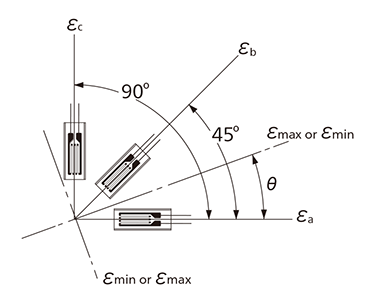
\includegraphics[width=3in]{images/Strain Gauge/Strain Gauge Orientation.png}
        \caption{Strain Gauge Orientation}
        \label{fig:Strain Gauge Orientation}
\end{figure}

\begin{gather}
    \varepsilon_{A} = (\frac{\varepsilon_{x} + \varepsilon_{y}} {2}) +  (\frac{\varepsilon_{x} - \varepsilon_{y}} {2})\cos({2\theta_{A}}) + \varepsilon_{xy}\sin({2\theta_{A}}) \\
    \varepsilon_{B} = (\frac{\varepsilon_{x} + \varepsilon_{y}} {2}) +  (\frac{\varepsilon_{x} - \varepsilon_{y}} {2})\cos({2\theta_{B}}) + \varepsilon_{xy}\sin({2\theta_{B}})\\
\varepsilon_{C} = (\frac{\varepsilon_{x} + \varepsilon_{y}} {2}) +  (\frac{\varepsilon_{x} - \varepsilon_{y}} {2})\cos({2\theta_{C}}) + \varepsilon_{xy}\sin({2\theta_{C}})
\end{gather}

\end{center} 


Electrically, strain gauges are resistors whose resistance changes based on how they deform.
This resistance change can be measured by a Wheatstone bridge.
\vspace{1em}

A Half-Bridge I configuration was chosen.
\begin{figure}[H]
    \centering
    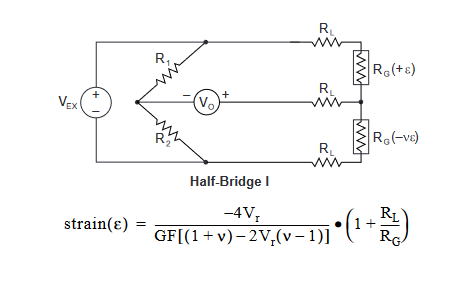
\includegraphics[width=5in]{images/calculating strain.png}
    \caption{Half-Bridge Resistor/Strain Gauge Configuration}
    \label{fig:hbi}
\end{figure}

\subsection{Strain Gauge Amplifier}
Since the voltage difference produced by a strain gauge in a Wheatstone bridge is very small (usually in a millivolts range), a strain gauge amplifier is used to amplify the voltage difference.
\vspace{1em}

For our strain gauge amplifier board, the HX711 was chosen because it is able to be powered off of 3.3V.
Additionally, we were able to find many reference schematics of HX711's used in strain gauge amplifiers, which aided in the development of our amplifier board.
\begin{figure}[H]
    \centering
    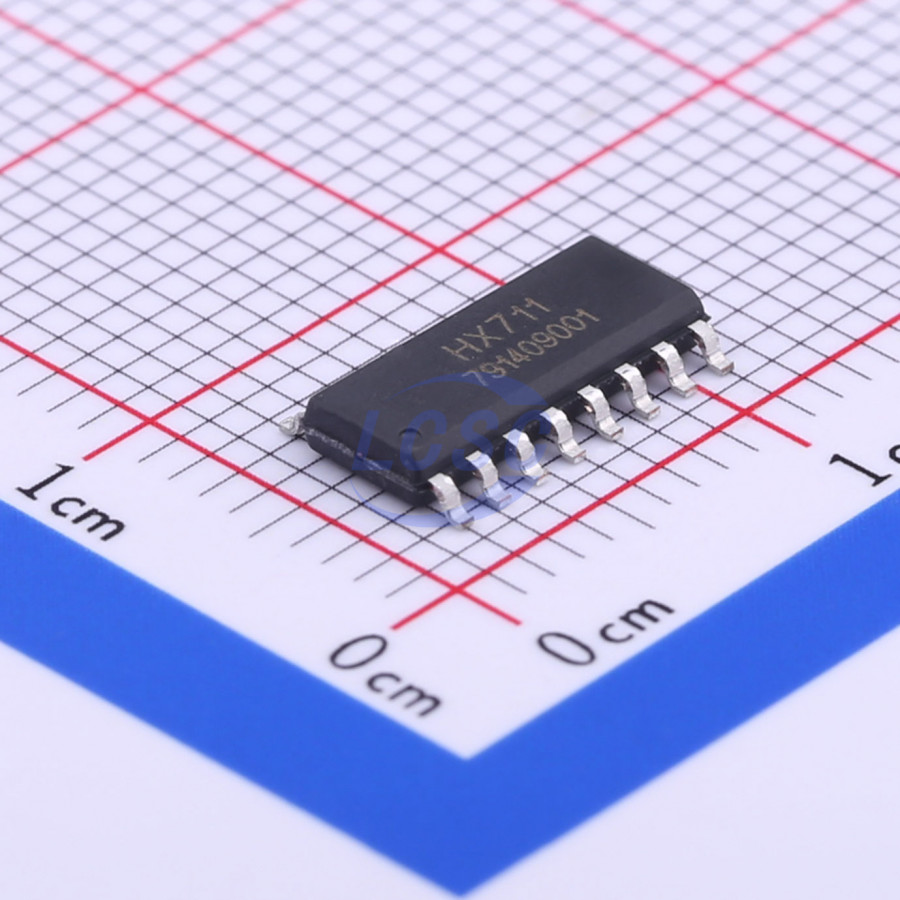
\includegraphics[width=2in]{images/hx711.jpg}
    \caption{HX711}
    \label{fig:hx711-pic}
\end{figure}

\subsection{Brake Pressure Sensor}
To measure the front and rear brake pressure, a media-isolated pressure transducer is used.
The brakes subteam selected for us Honeywell's MIPAG1XX050BSAAX.
This ratiometric sensor can measure pressure up to 50 bar, and uses a sealed gage pressure reference.
Its transfer function is defined to as
\begin{gather}\label{eq:bps}
    V_O = \frac{0.8\times V_S}{P_{max}-P_{min}}\times(P_{applied}-P_{min})+0.1\times V_S
\end{gather}
Where $V_O$ is the output voltage in V, $V_S$ is the voltage supply in V, $P_{applied}$ is the measured pressure, and $P_{max},P_{min}$ are the maximum and minimum pressures defined as $0.9\times V_S$ and $0.1\times V_S$ respectively.

It is important to note that this sensor runs off of 5V, so a voltage divider to step the maximum output down to 3.3V is required for the Teensy 4.0 to interface with it.
Additionally, the specific sensor model chosen interfaces with a Aptiv Metri Pack 150 connector.
\begin{figure}[H]
    \centering
    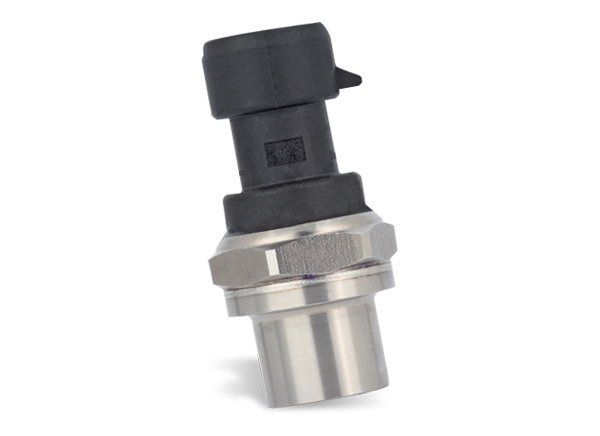
\includegraphics[width=2in]{images/mips.png}
    \caption{Honeywell MIPAG1XX050BSAAX}
    \label{fig:mips}
\end{figure}

\subsection{GPS Module}
A GPS module is used to collect data about SDM-23's position and velocity.
This can then be used to calculate laps and lap times, get a good idea of the top speed, and relate data channels such as lateral acceleration to track location.
The module used is the Adafruit Ultimate GPS Breakout, pictured in \ref{fig:gps} which is built around the MTK3339 chipset.

It is important to note that the position data is in degrees and minutes in the following format:
\begin{itemize}
    \item Latitude: DDMM.MMMM
    \item Longitude: DDDMM.MMMM
\end{itemize}
Interally these are stored as floating-point numbers.
These can be converted into decimal degrees by
\begin{gather}
    D_{decimal} = D+M/60
\end{gather}
Where $D$ and $M$ are the degrees and minutes values obtained from the module, and $D_{decimal}$ is decimal degrees.
\begin{figure}[H]
\centering
    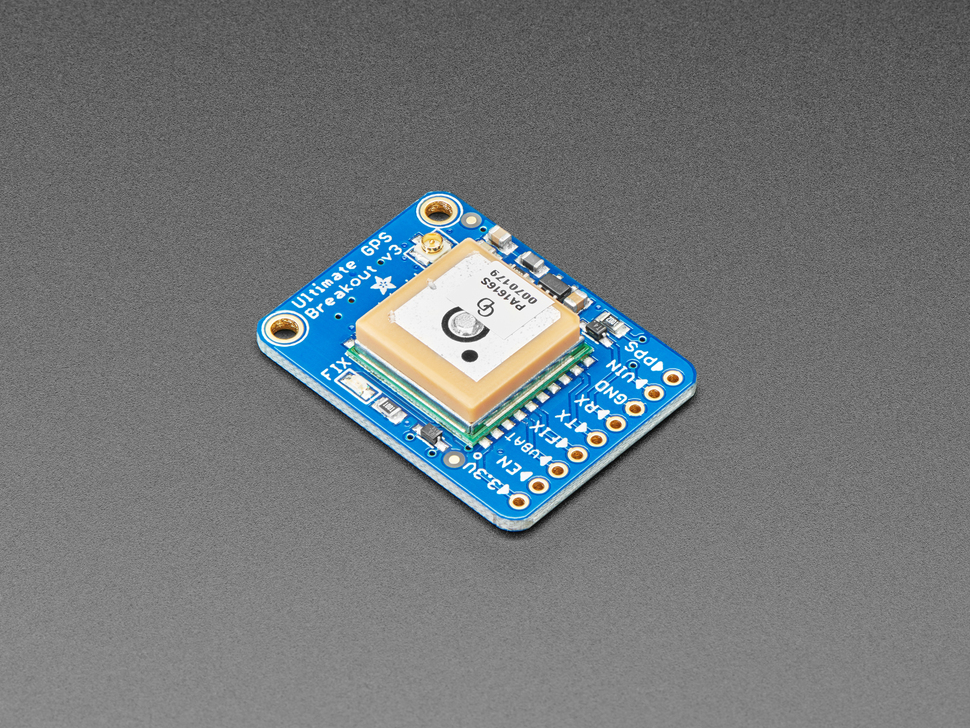
\includegraphics{images/gps.jpg}
    \caption{Adafruit Ultimate GPS Breakout}
    \label{fig:gps}
\end{figure}
An active external antenna is also used to increase the GPS Module's gain.


\chapter{Methodology}
This chapter will go over methods and procedures used in the development of the DAQ system.
\section{Research and Design Phase}
\subsection{Research Phase}
During the research phase an exhaustive literature review was conducted.
When reviewing the designs for DAQ and GLV systems of other FSAE teams, the following points were looked for, in rough order of priority:
\begin{enumerate}
    \item Sensor and connector selection
    \item Methodology
    \item Overall system design
\end{enumerate}

\subsection{Electrical Design}
The DAQ package requires many components to be connected to different boards located throughout the car.
A spreadsheet was used to keep track of all components, their operating voltages, current draw, what microcontroller pin they would be accessible on, and which board they would be connected to.
\begin{figure}[H]
        \centering
        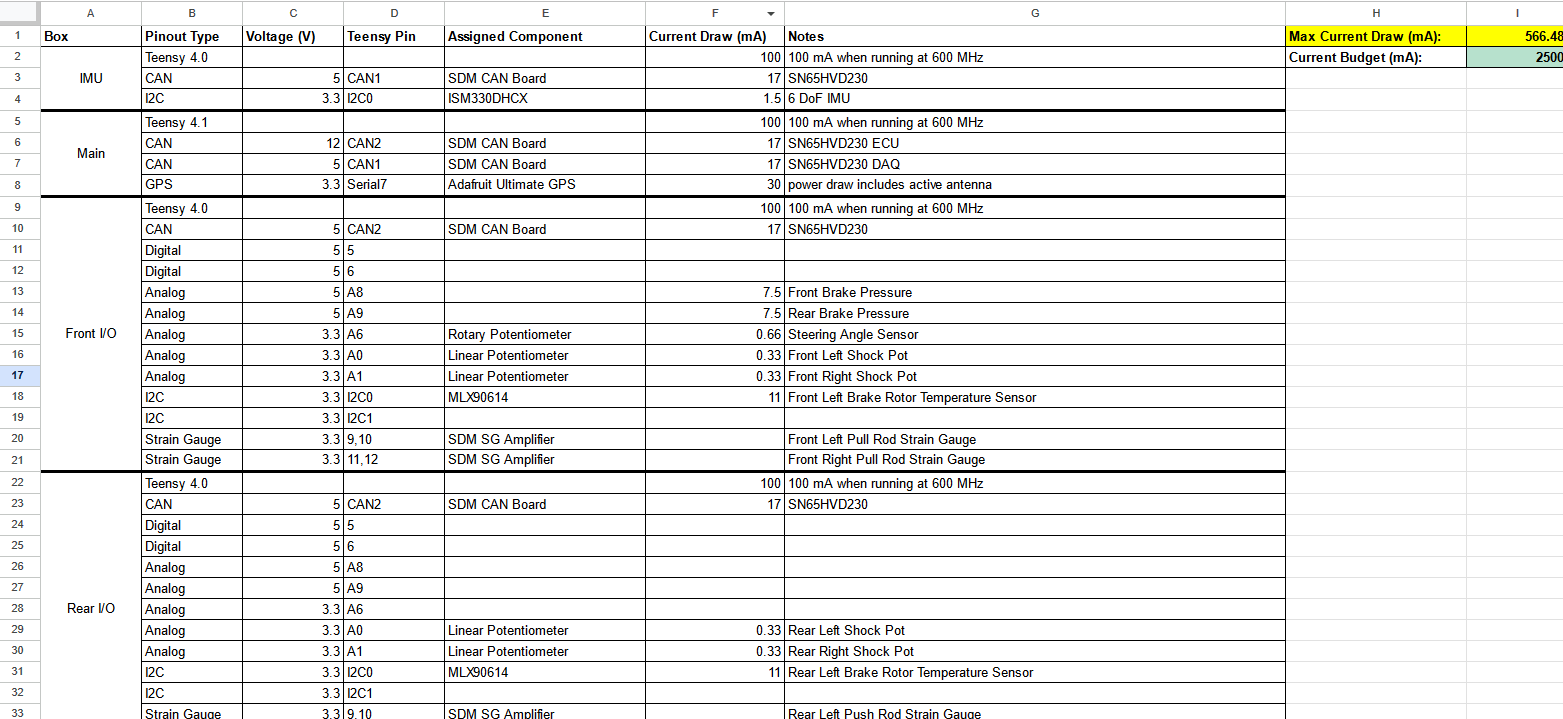
\includegraphics[width=7in]{images/electricalplanning.png}
        \caption{Component Planning Spreadsheet}
        \label{fig:ep}
\end{figure}


\subsection{Software Design}
PlatformIO, a VS Code extension, was used to develop software for the Teensy 4.1 and Teensy 4.0.
It is functionally equivalent to the Arduino IDE, while having the benefits of using a professional text editor such as VS Code.
Although not exclusive to PlatformIO, using this platform (i.e. Teensyduino) allows us to use Arduino functions and libraries for the Teensy boards, which greatly sped up software development.

\subsubsection{CAN Protocol Design}
The DAQ CAN bus will have to handle multiple channels of data of varying sizes.
Each CAN message contains 8 bytes of data, which is more than enough for one channel.
As such, some data channels, when encoded smartly, can be combined into a single message.
\vspace{1em}

The CAN protocol is described in a spreadsheet located on the team's Google Drive.
It includes information such as the CAN message ID, which component is sending the message, if it is signed or unsigned, the data channel being encoded, its units, and how to encode and decode the data.
Since the DAQ CAN bus is separate from the ECU's, message IDs that conflicted with the Haltech CAN protocol were not an issue.
\begin{figure}[H]
        \centering
        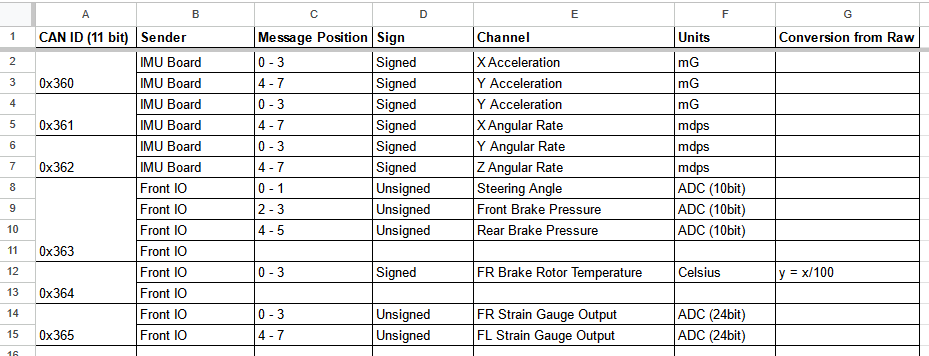
\includegraphics[width=6.5in]{images/canplanning.png}
        \caption{CAN Planning Spreadsheet}
        \label{fig:cpslol}
\end{figure}
\subsection{Hardware Design}
To simplify hardware designs and part orders, only M3 and 8-32 screws are used, unless a different size was required.


\section{Manufacturing Phase}
All printed circuit board (PCB) designs were created using KiCad and sent to JLCPCB for manufacturing.
Unless otherwise mentioned, any SMT assembly required were also done by JLCPCB.
Enclosures and sensor mounts were created using SOLIDWORKS and were either sent to AEI Industries for laser cutting with 6061 aluminum or 3D printed at ASU using PETG and PLA.

\subsection{Wiring and Pinout Documentation}
Three spreadsheets were maintained for wiring manufacturing:
\begin{itemize}
    \item Wire color conventions
    \item Wire length and assembly status
    \item Pinout documentation
\end{itemize}
The color convention spreadsheet showed all possible wire colors for each type of connection.
\begin{figure}[H]
        \centering
        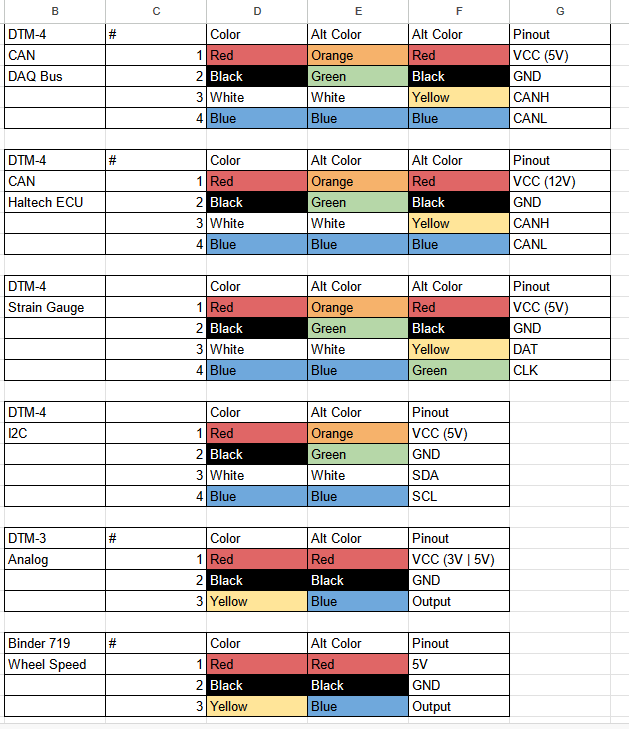
\includegraphics[width=5in]{images/colors.png}
        \caption{Wire Color Conventions}
        \label{fig:asfsfsfsfsfsfsf}
\end{figure}
The wire length spreadsheet showed the assembly status of each cable, and kept track of its length in CAD, how much to cut (CAD length plus $10\%$), and how much was actually cut.
\begin{figure}[H]
        \centering
        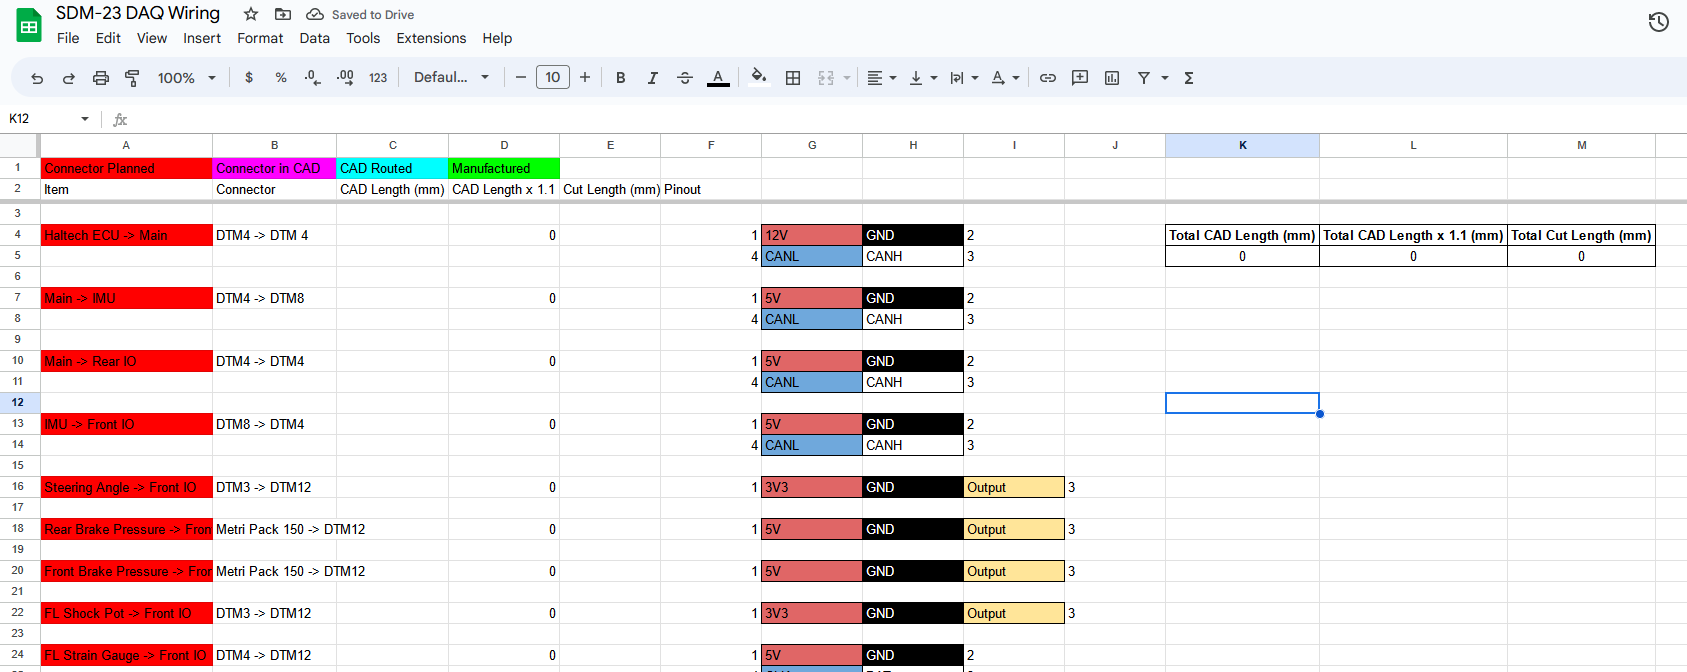
\includegraphics[width=7in]{images/wiring.png}
        \caption{Wire Length Tracking}
        \label{fig:fffsaf}
\end{figure}
The pinout spreadsheet documented what each pin should be connected to.
\begin{figure}[H]
        \centering
        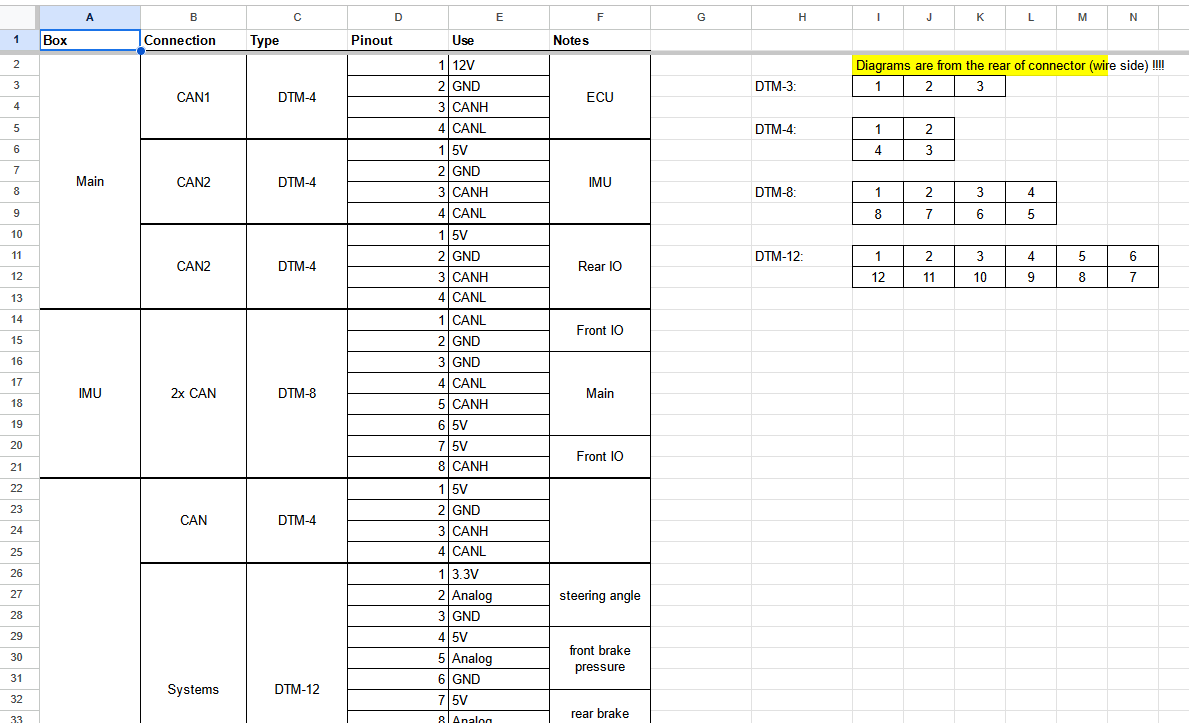
\includegraphics[width=7in]{images/pinouts.png}
        \caption{Box Pinout Documentation}
        \label{fig:hghahhhh}
\end{figure}
These three spreadsheets were instrumental while assembling the connectors and debugging any issues.


\subsection{Strain Gauge Integration}
\subsubsection{Materials and Chemicals Required to Bond the Strain Gauge}
Bonding the MMF403924 Tee Rosette strain gauges required the following:
\begin{itemize}
    \item Personal protective equipment (PPE)
    \item M-Bond 200 Adhesive
    \item M-Bond 200 Catalyst C
    \item M-Prep Conditioner A
    \item M-Prep Neutralizer 5A
\end{itemize}

\subsubsection{Personal protective equipment (PPE)}

Taken directly from the following data sheets: 
\begin{itemize}
    \item M-Bond\textunderscore 200\textunderscore Adhesive\textunderscore SDS\textunderscore V3.0.pdf
    \item M-Bond\textunderscore 200\textunderscore Catalyst\textunderscore C\textunderscore SDS\textunderscore V3.0.pdf
    \item M-Prep\textunderscore Conditioner\textunderscore A\textunderscore SDS\textunderscore V2.pdf
    \item M-Prep\textunderscore Neutralizer\textunderscore 5A\textunderscore SDS\textunderscore V2.pdf
\end{itemize}
\begin{quote} 
``Wear protective eye glasses for protection against liquid splashes. Wear eye protection with side protection. (Recommended: EN166)."
\end{quote}
\begin{quote} 
``Wear impervious gloves. Recommended: Equivalent or similar to EN374.
Gloves should be changed regularly to avoid permeation problems."
\end{quote}
\begin{quote} 
``Body protection:
Wear impervious protective clothing, including boots, lab coat, apron or coveralls,
as appropriate, to prevent skin contact.
Use only in well-ventilated areas. In case of inadequate ventilation wear respiratory protection.
For large quantities - A suitable mask with filter type A may be appropriate.
(Recommended: EN141 or EN405)"
\end{quote}

\subsubsection{M-Bond 200 Adhesive}
Chemical name(s): Ethyl 2-cyanoacrylate
\vspace{1em}

Use case: Adhesives
\begin{figure}[H]
        \centering
        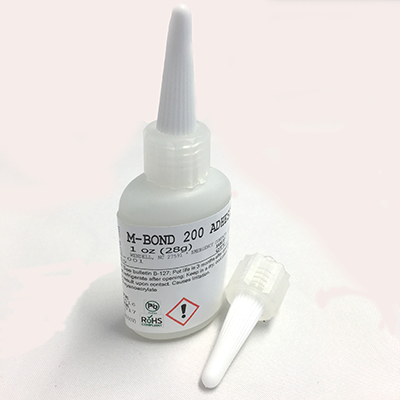
\includegraphics[width=3in]{images/Strain Gauge/M-Bond 200 Adhesive.png}
        \caption{M-Bond 200 Adhesive}
        \label{fig:M-Bond 200 Adhesive}
\end{figure}

\subsubsection{M-Bond 200 Catalyst C}
Chemical name(s): Propan-2-ol and N-Phenyldiethanolamine

\vspace{1em}

Use case: Adhesives
\begin{figure}[H]
        \centering
        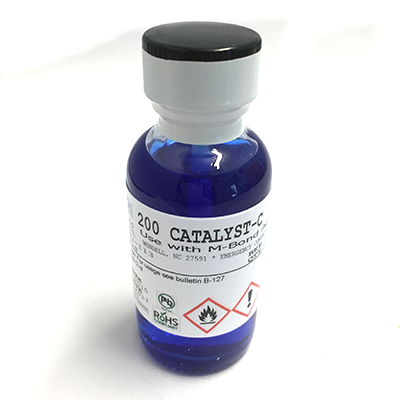
\includegraphics[width=3in]{images/Strain Gauge/M-Bond 200 Catalyst C.png}
        \caption{M-Bond 200 Catalyst C}
        \label{fig:M-Bond 200 Catalyst C}
\end{figure}

\subsubsection{M-Prep Conditioner A}
Chemical name(s): Phosphoric Acid

\vspace{1em}

Use case: PC14 Metal surface treatment products, including galvanic and electroplating products

\begin{figure}[H]
        \centering
        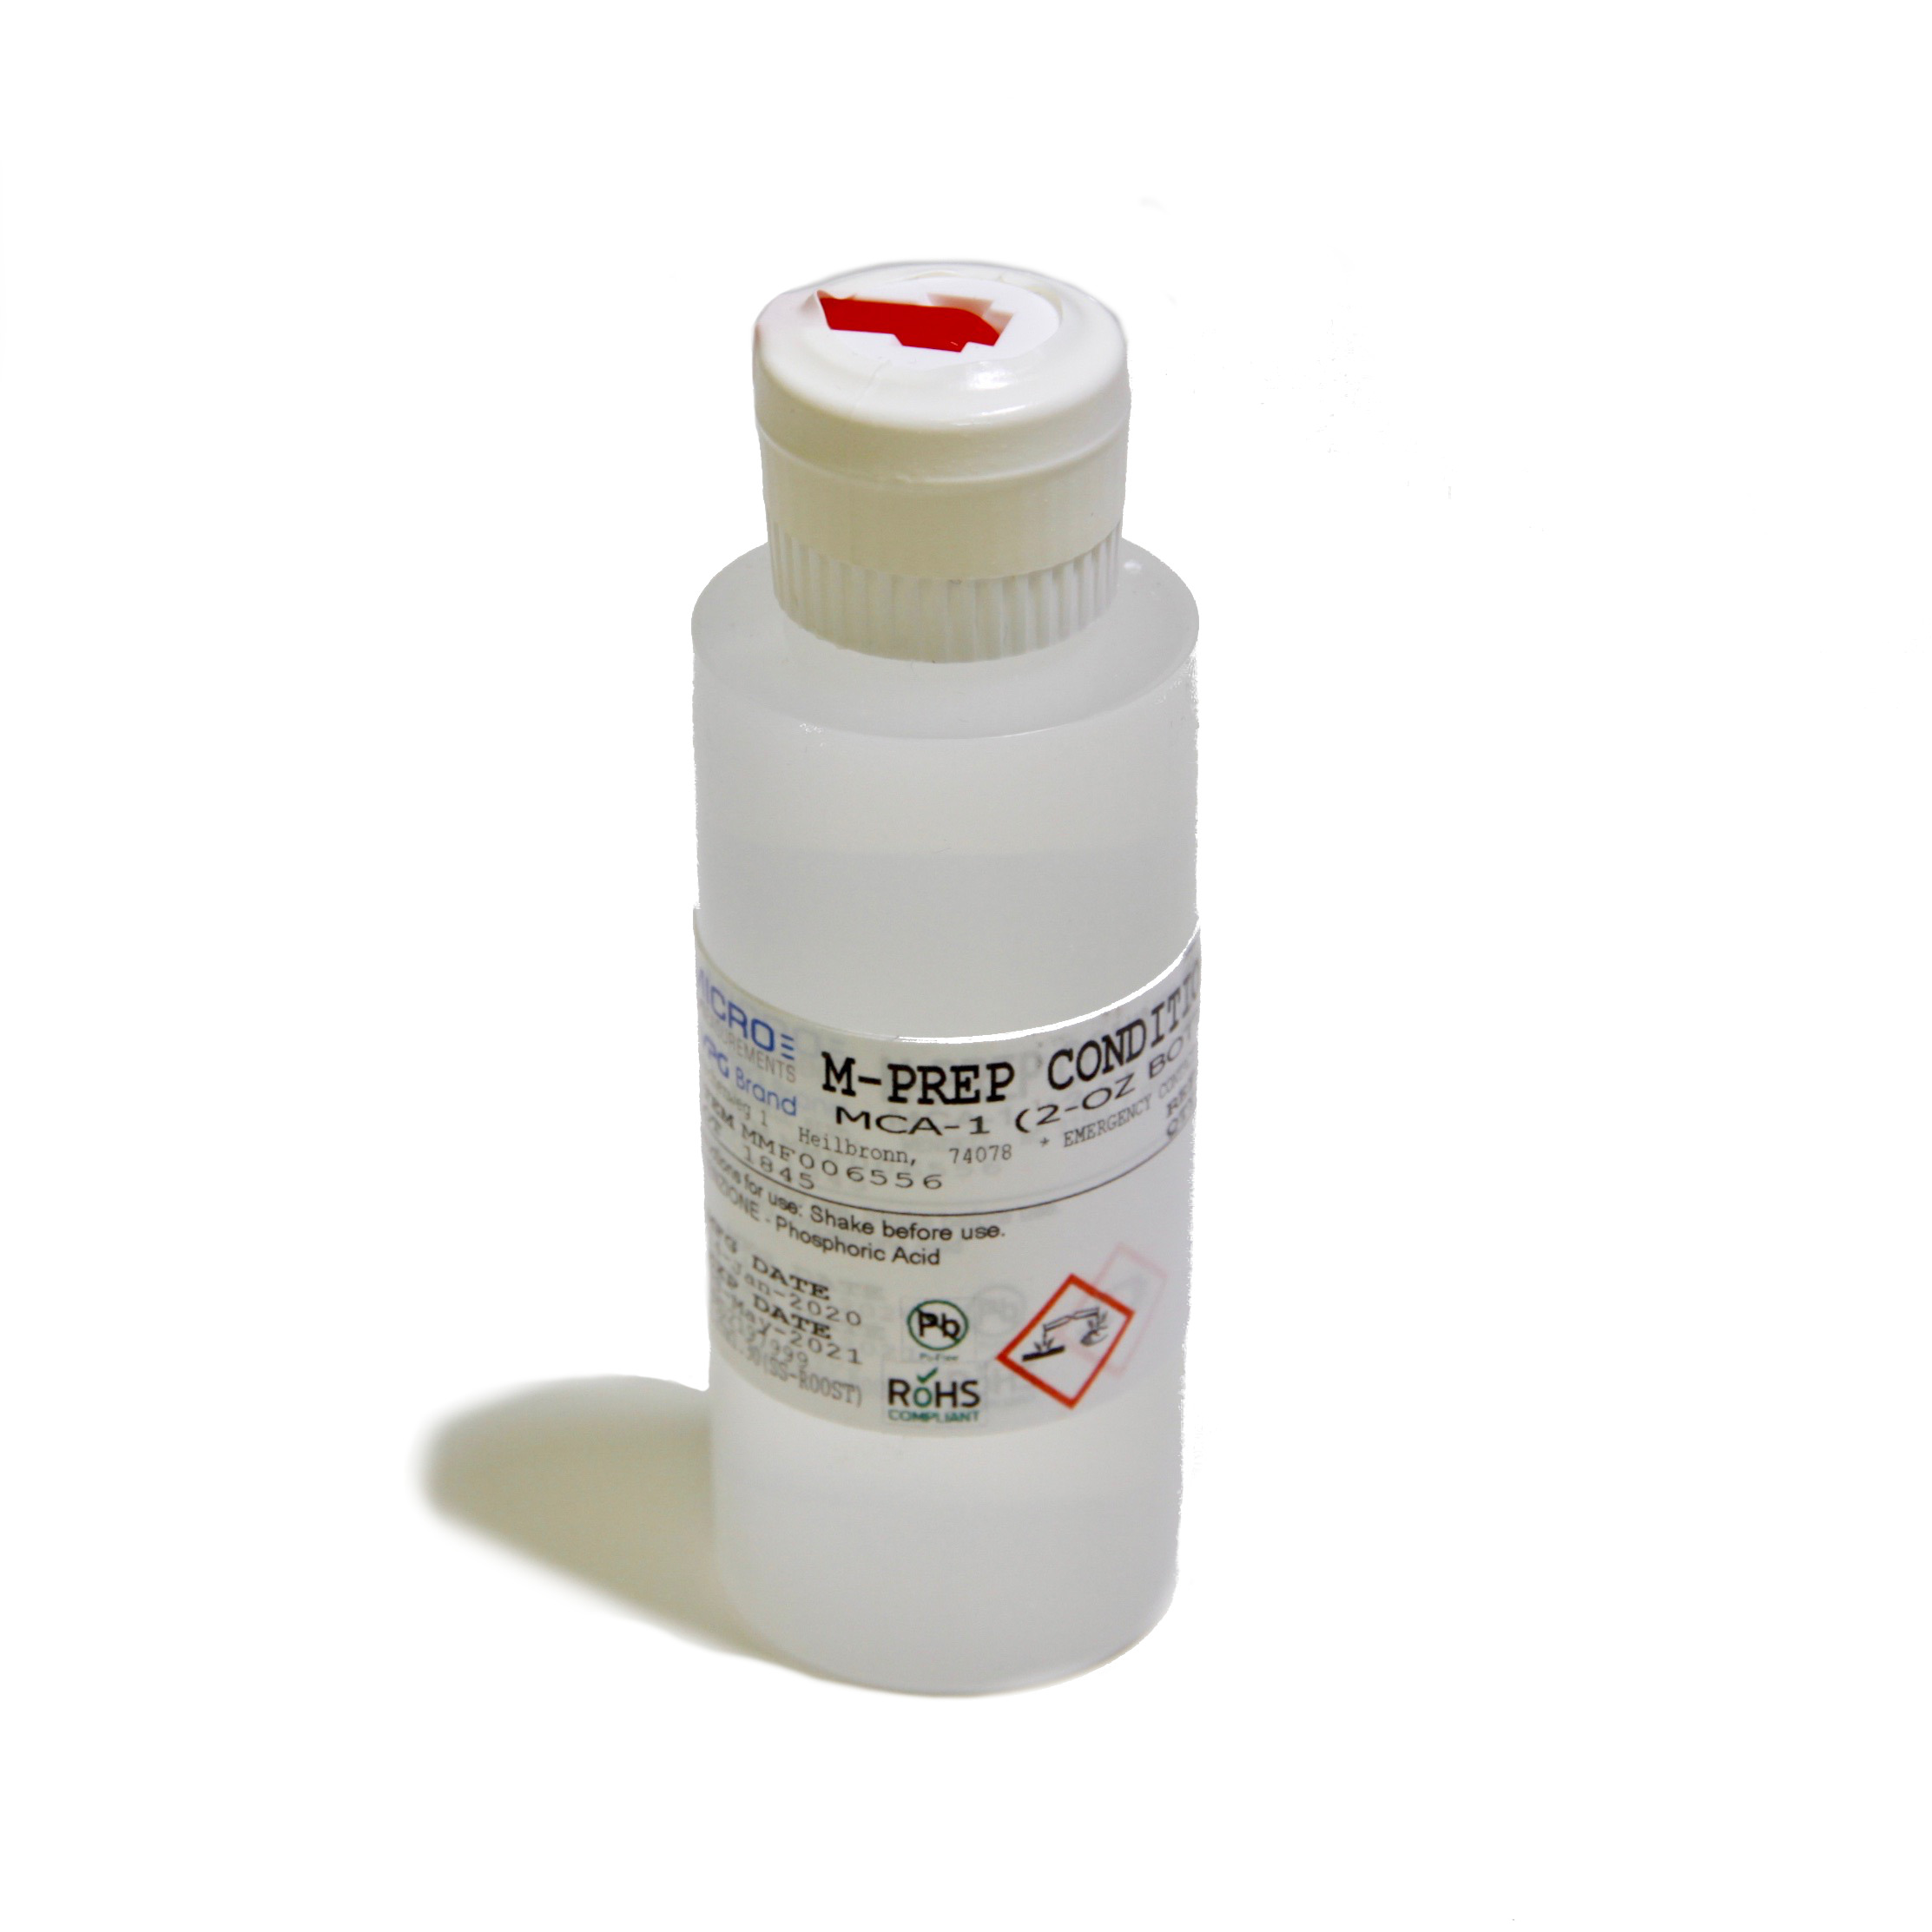
\includegraphics[width=3in]{images/Strain Gauge/M-Prep Conditioner A.jpg}
        \caption{M-Prep Conditioner A}
        \label{fig:M-Prep Conditioner A}
\end{figure}

\subsubsection{M-Prep Neutralizer 5A}
Chemical name(s): Sodium tetraborate pentahydrate 

\vspace{1em}

Use case: PC14 Metal surface treatment products, including galvanic and electroplating products
\begin{figure}[H]
        \centering
        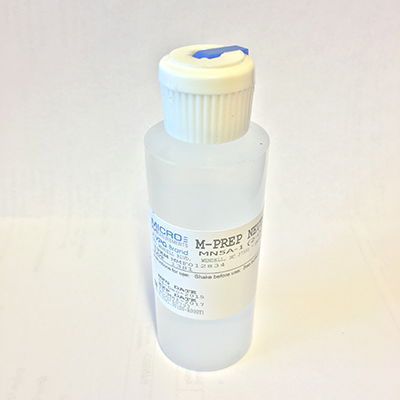
\includegraphics[width=3in]{images/Strain Gauge/M-Prep Neutralizer 5A.png}
        \caption{M-Prep Neutralizer 5A}
        \label{fig:M-Prep Neutralizer 5A}
\end{figure}


\subsubsection{Bonding Process}
According to Instruction Bulletin B-127: Strain Gage Installations with M-Bond 200 Adhesive there are 11 steps needed to bond the gauges. They are as follows.
\vspace{1em}
\begin{enumerate}
    \item Degreasing the bonding suface with CSM Degreaser or GC-6 Isopropyl Alcohol.
    \item "Preliminary dry abrading with 220- or 320-grit silicon-carbide paper is generally required if there is any surface scale or oxide. Final abrading is done by using 320-grit silicon-carbide paper on surfaces thoroughly wetted with M-Prep Conditioner A; this is followed by wiping dry with a gauze sponge. Repeat this wet abrading process with 400-grit silicon-carbide paper, then dry by slowly wiping through with a gauze sponge" (Instruction Bulletin B-127)
    \item Using M-Prep Neutralizer 5A and cotton tip apply to the intended bonding area. Then use a gauze to slowly dry the surface making sure to not wipe back and forth as this could recontaminate the surface.
    \item Using a pair of tweezers extract the Tee Rosette strain gauge from the envelope placing it bonding side down. The tape the gauge. Slowly lift the tape at roughly at a  45 degree angle.
    \item Tape the gauge onto the bonding surface.
    \item Lift the tape at roughly at a 45 degree angle making sure "the specimen approximately 1/2 in [10 mm] beyond the terminal."
    \item The following three steps need to be performed within 3 to 5 seconds.
    \item Apply a sparingly amount of M-Bond 200 catalyst to the strain gauge. 
    \item Apply about one to two drops of the M-Bond 200 adhesive to the corner of the lifted tape area. For curved surfaces like a rod apply a very small amount to avoid the substance from dripping. 
    \item Immediately flip the tape. Then using a gauze wipe the tape in a single stroke.
    \item Apply pressure with your thumb to area that the gauge was bonded to. Hold this pressure for about a minute. The longer the better though as removing your thumb too soon could cause the bond to be very weak. For example, when lifting the tape the gauge could peel off. Note: If the gauges are large or if the surface is curved one should wait two minutes instead of one.
    \item It is not required to remove the tape immediately. In fact unless you are soldering or adding something like a  coating you should leave the tape on. When ready to remove the tape slowly peel it directly over itself. This will prevent the gauge from being damaged or lifted with the tape. 
\end{enumerate}

"FINAL INSTALLATION PROCEDURE":
Solder the gauges. 
Remove any solder flux. 
Apply protective coating.


\subsubsection{Bonded and Soldered Strain Gauges}
\begin{figure}[H]
        \centering
        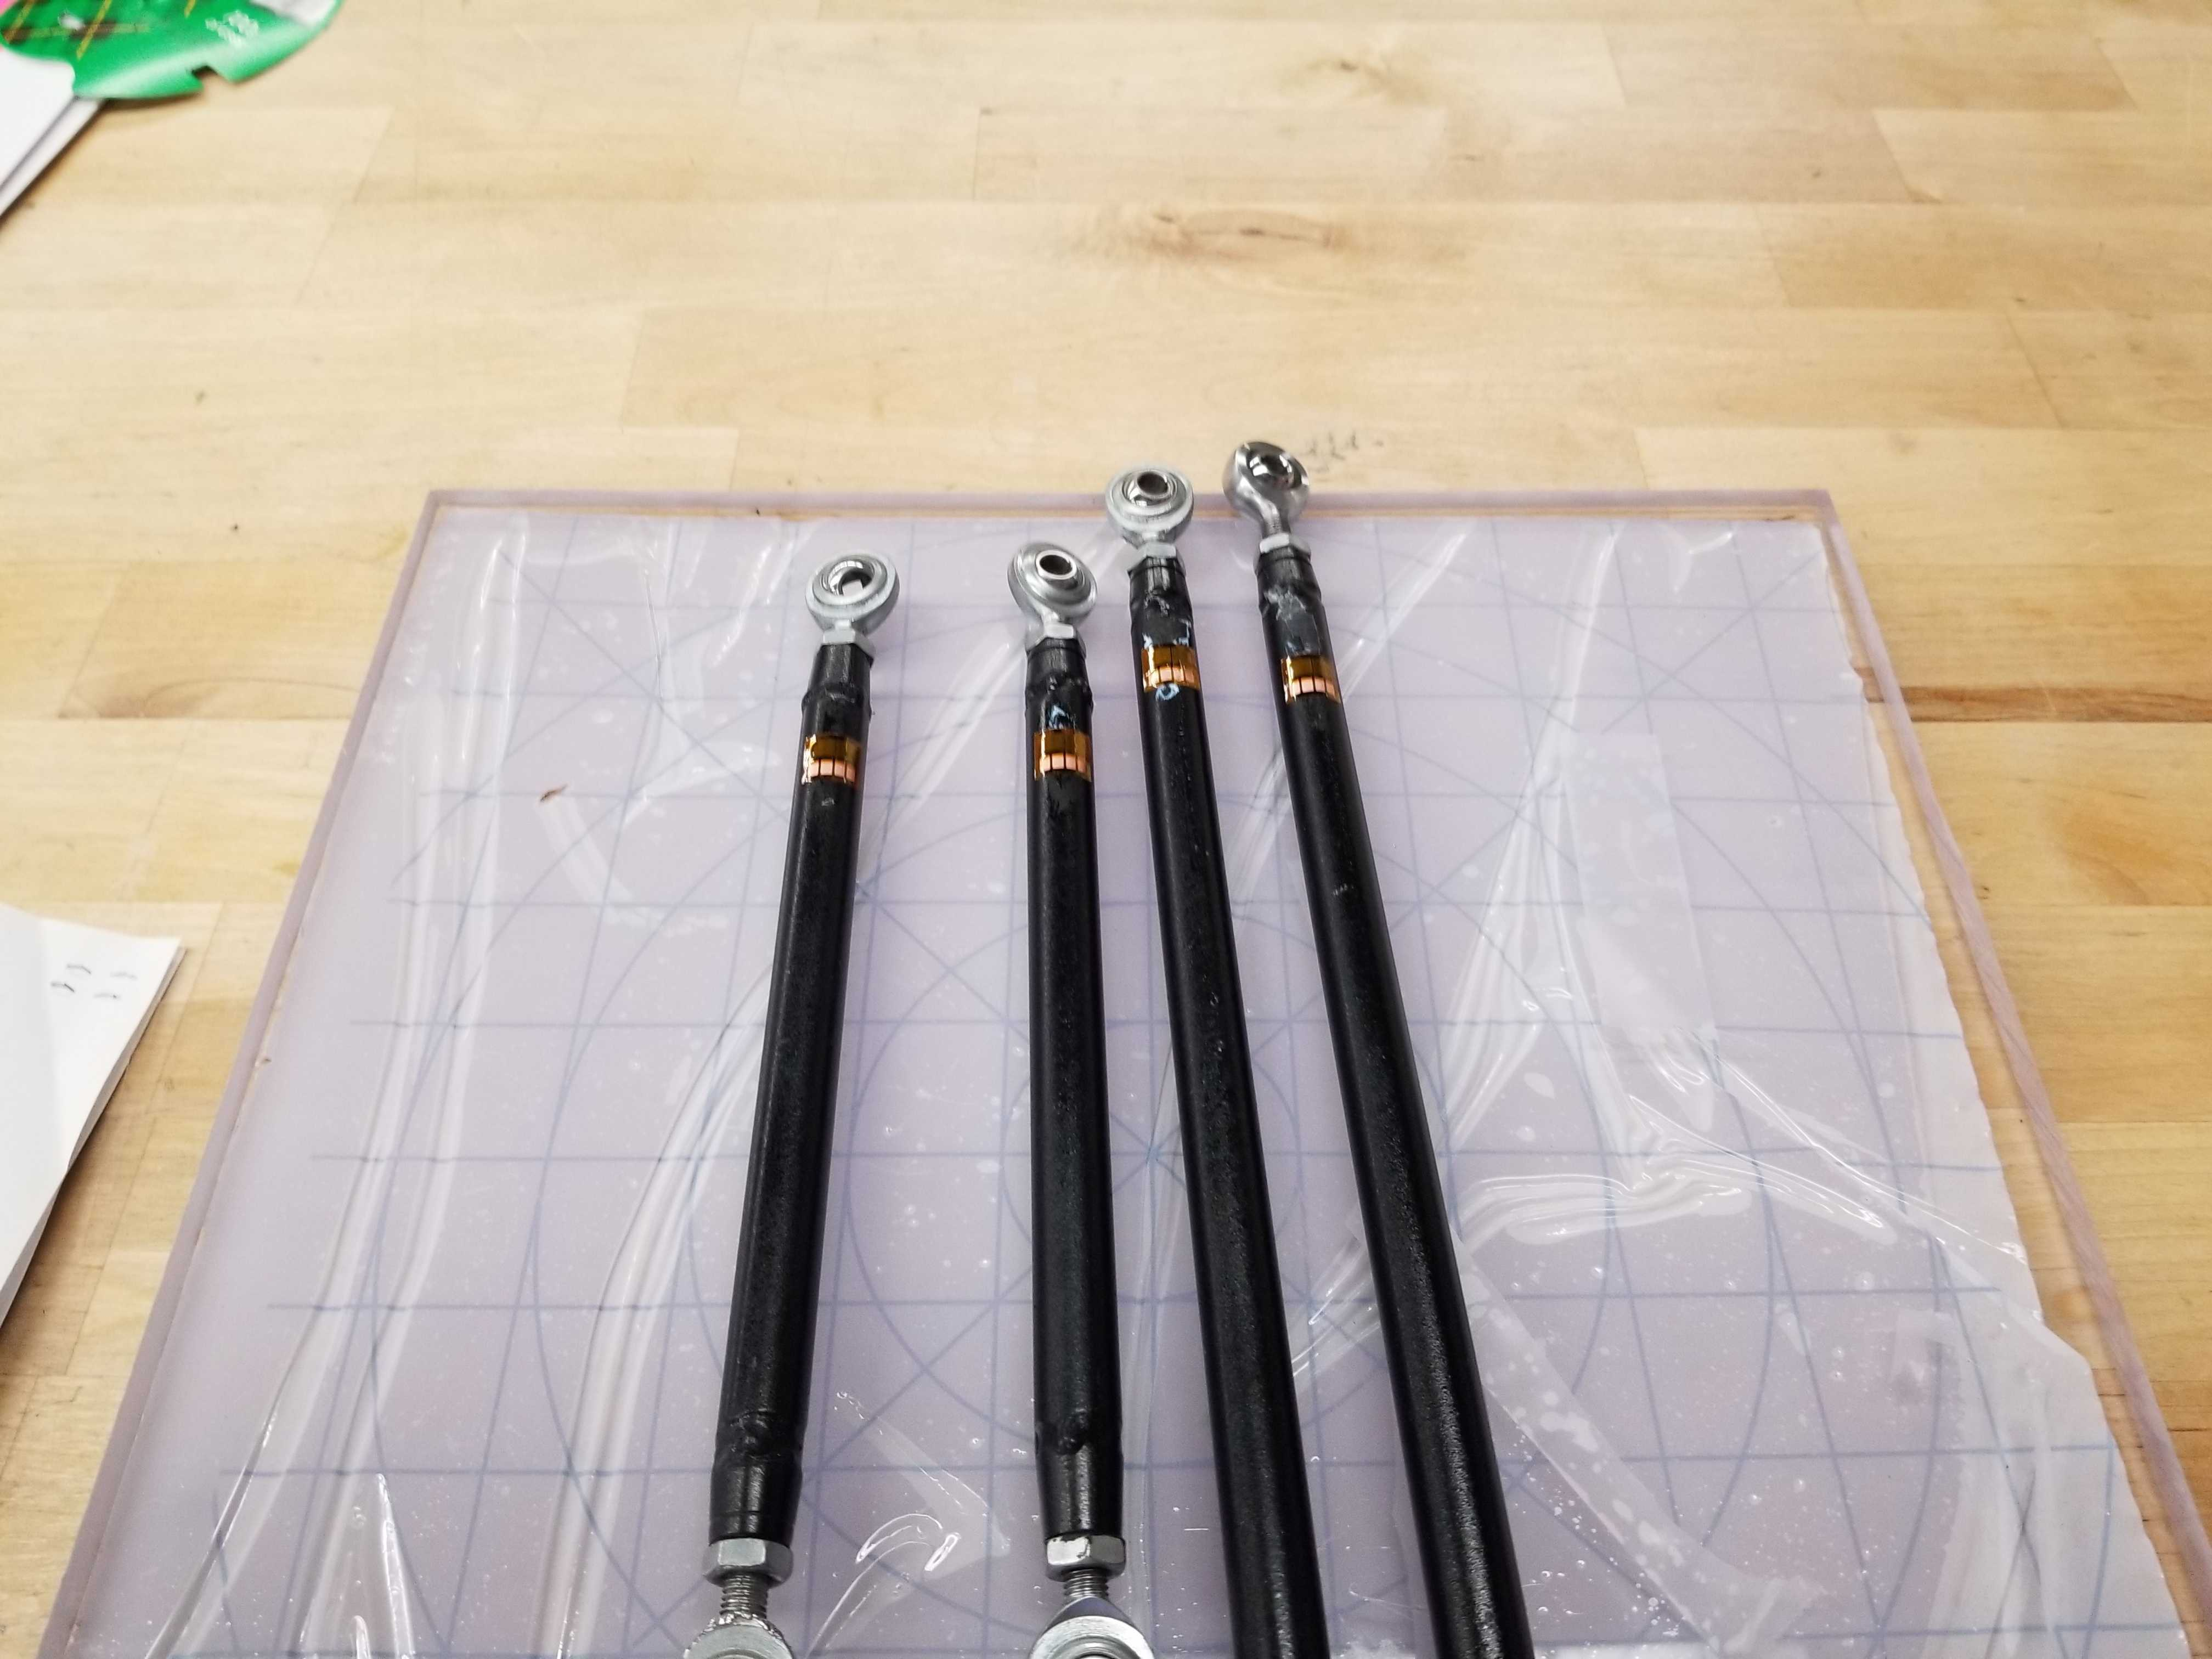
\includegraphics[width=4in]{images/Strain Gauge/straingauge-noleads.jpg}
        \caption{Bonded Strain Gauges}
        \label{fig:straingauge-noleads}
\end{figure}

\begin{figure}[H]
        \centering
        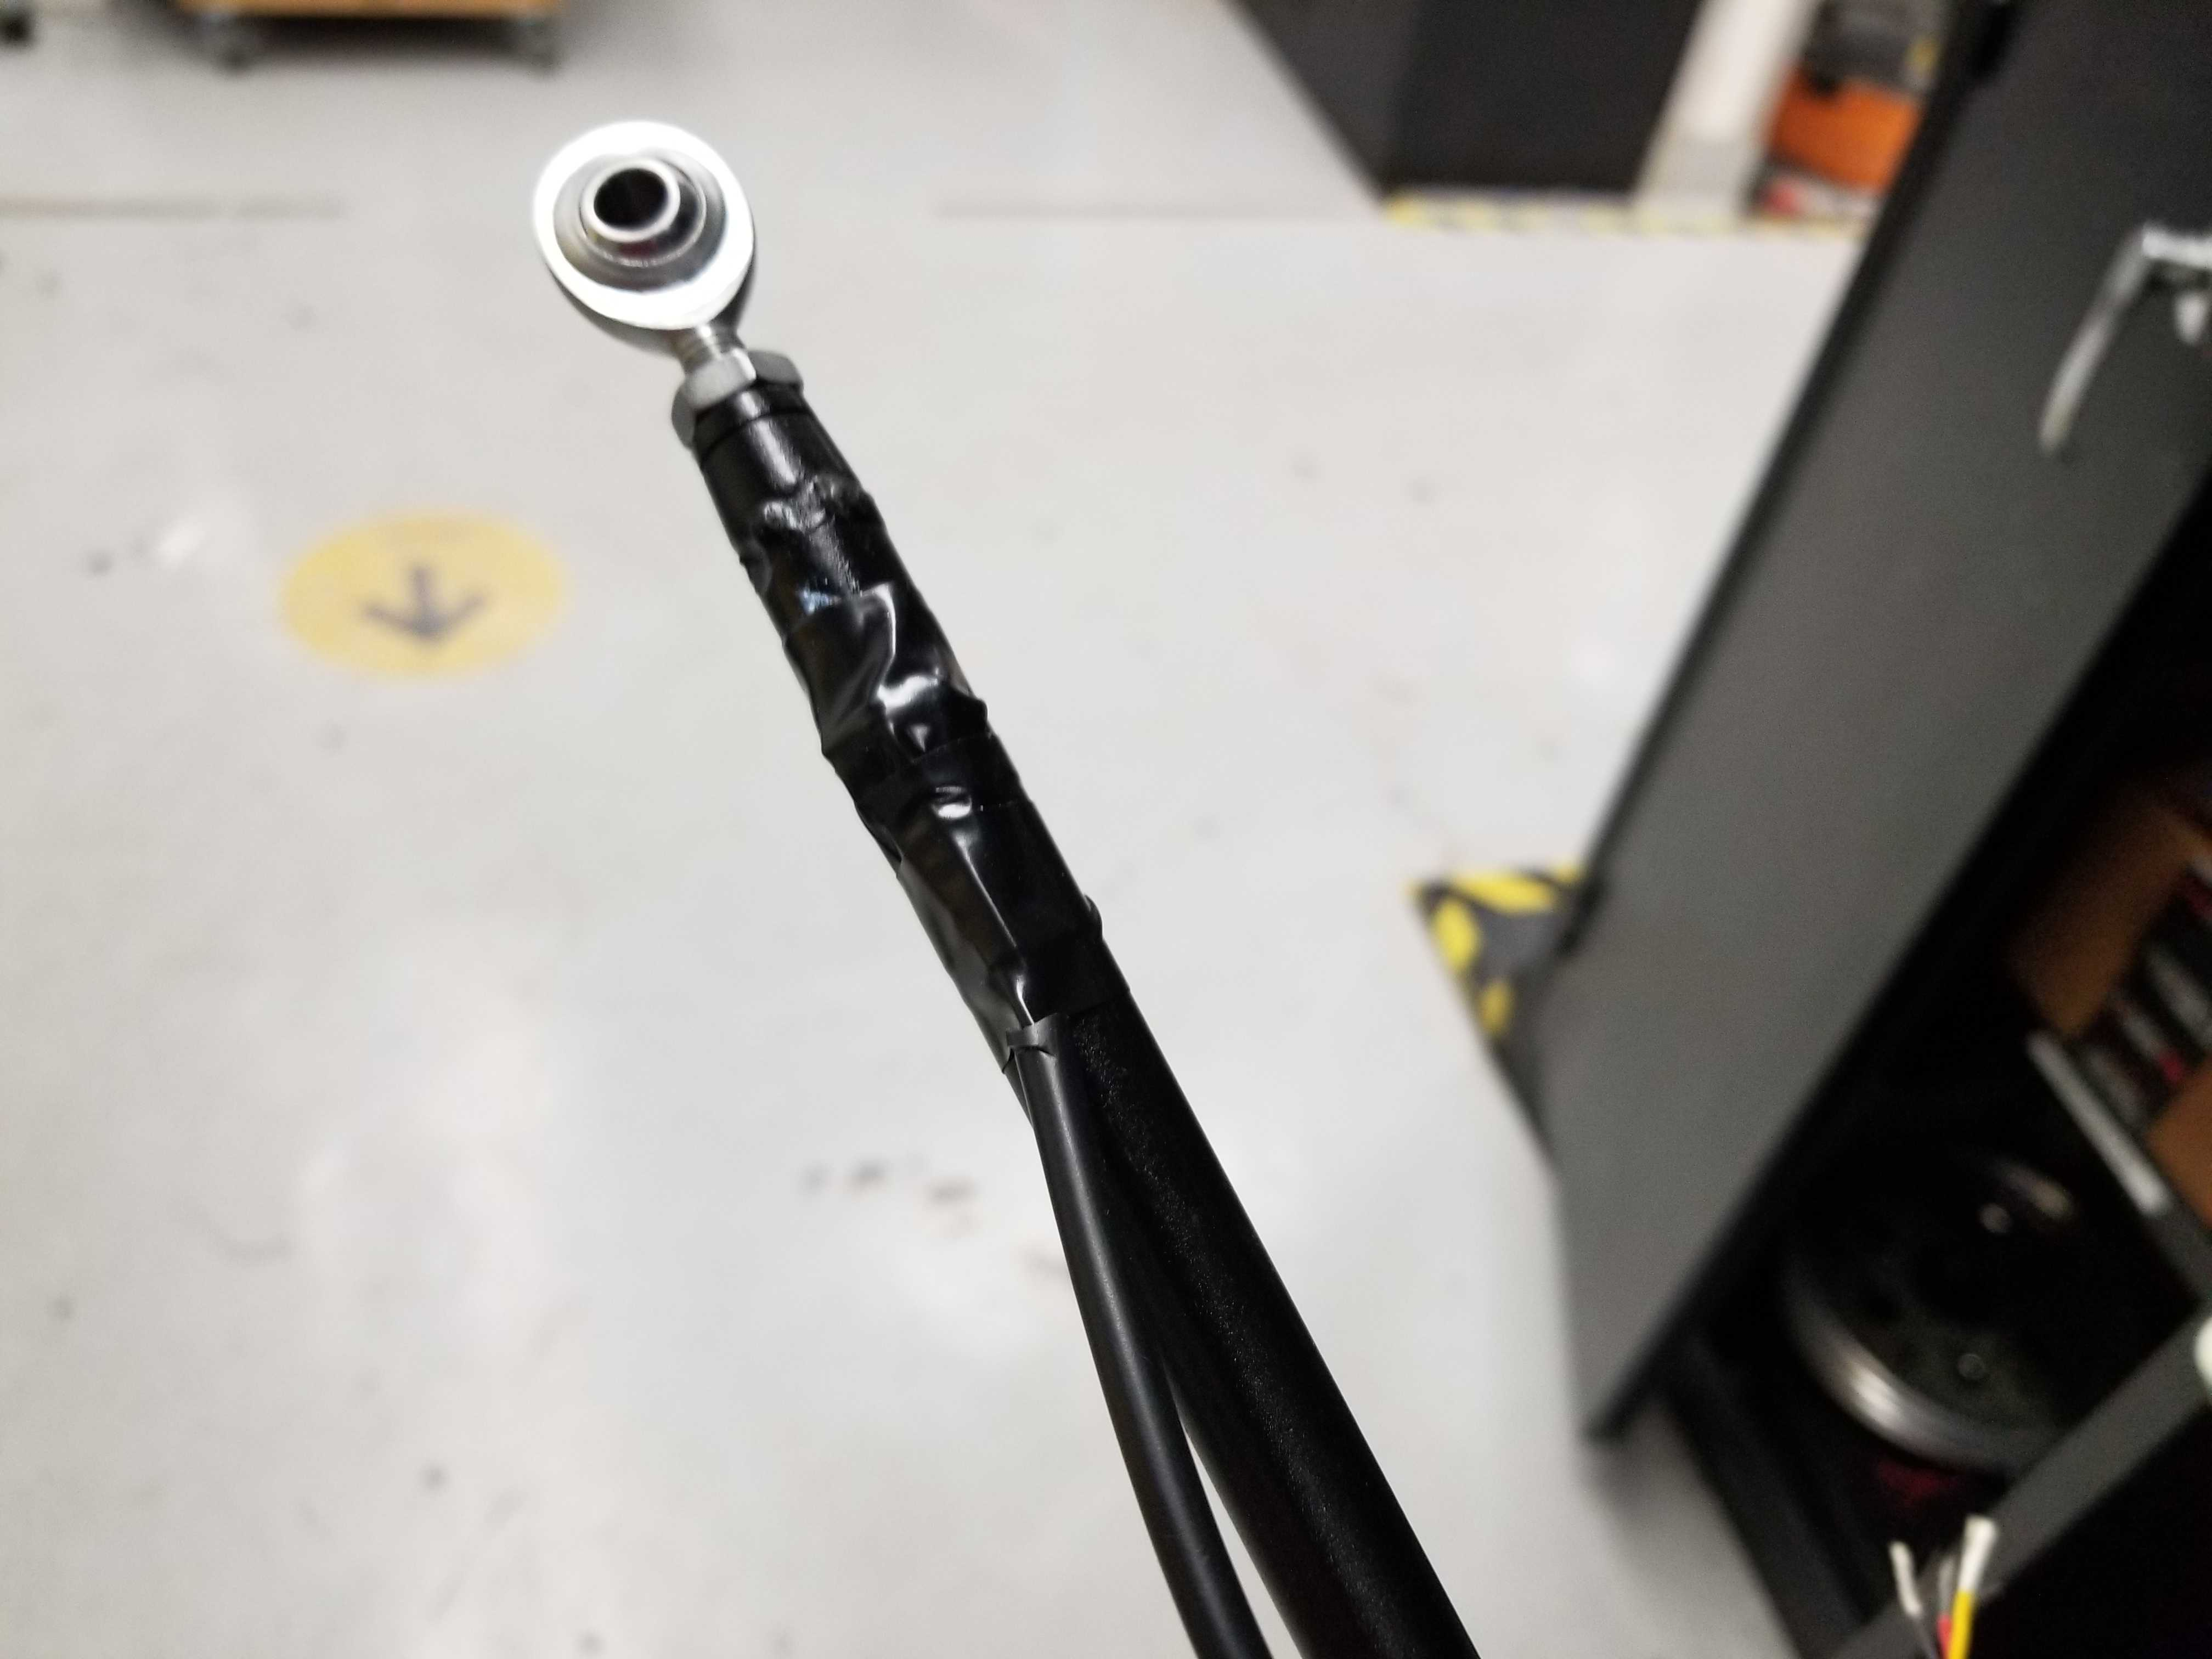
\includegraphics[width=4in]{images/Strain Gauge/straingauge.jpg}
        \caption{Soldered Strain Gauges}
        \label{fig:Soldered Strain Gauges}
\end{figure}


\subsection{Box Assembly}
All 3D-prints were printed by a Creality Ender 3 Pro.
Terminal blocks were screwed in by using electrical tweezers.
The DTM connectors were super glued to their 3D-printed panel mounts.

\chapter{Engineering Design}
The engineering design chapter will detail the low-level design of each DAQ component as well as the integration of the system as a whole.

\section{System Design Overview}
The package is split into electronics to be installed on the car, and a set of software tools and scripts used to extract and analyse the data collected.

\begin{figure}[H]
    \centering
    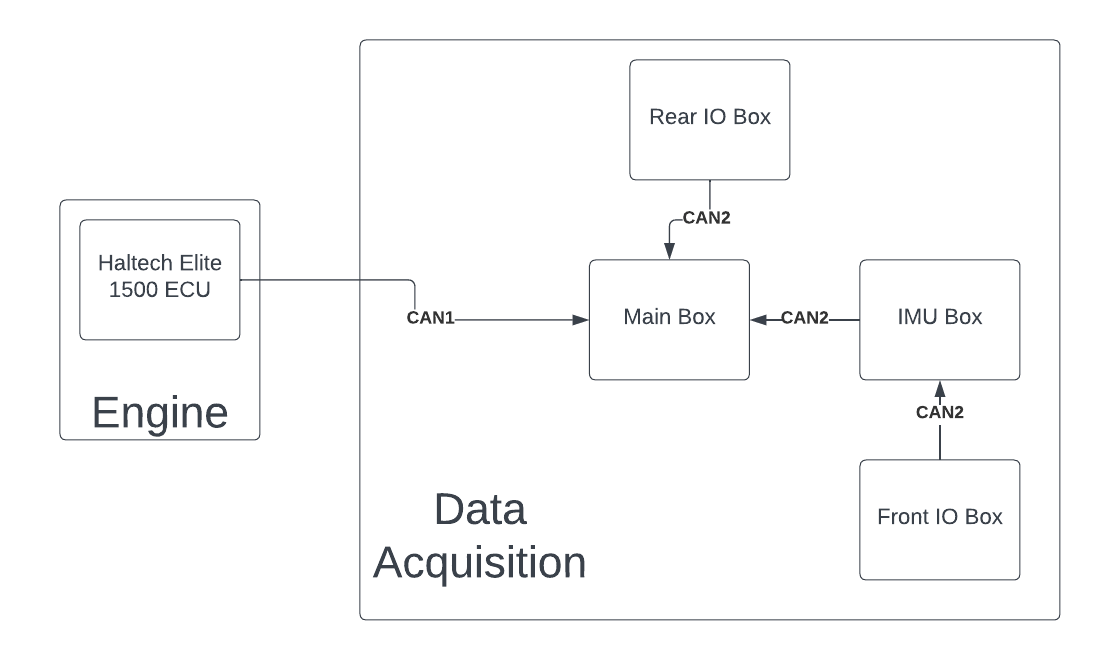
\includegraphics[width=6in]{images/SDM-23 System.png}
    \caption{SDM-23 DAQ Electrical System Block Diagram}
    \label{fig:sdm23-systemdiagram}
\end{figure}
The system block diagram in Figure \ref{fig:sdm23-systemdiagram} displays the high level components of the DAQ electrical system as well as their interfaces with each other and other electrical components in the car.
It also shows which subteam is responsible for each electrical component.
All of the DAQ components are composed of at least a custom PCB and 3D printed housing.
\vspace{1em}

The main box is the central component in SDM-23.
It is a standalone data logger that features two separate CAN bus interfaces, one used for interfacing with the Haltech ECU and the second used for interfacing with the other DAQ components, a GPS module, and a 5V regulator to step down the 12V it receives from the ECU.
\vspace{1em}

The IMU box has two functions: collecting and reading data from the ISM330DHCX, and transmitting it over CAN.
\vspace{1em}

The front and rear I/O boxes are responsible for interfacing with the majority of SDM-23's sensors and transmitting them over CAN.
For instance, the front right brake rotor temperature sensor and steering angle sensor are connected to the Front I/O box.

\section{Software Design}
The software for the SDM-23 DAQ system is relatively simple.
Figure \ref{fig:sdmioafsdasfs} shows a state diagram for the software for the IMU and IO boxes.
\begin{figure}[H]
    \centering
    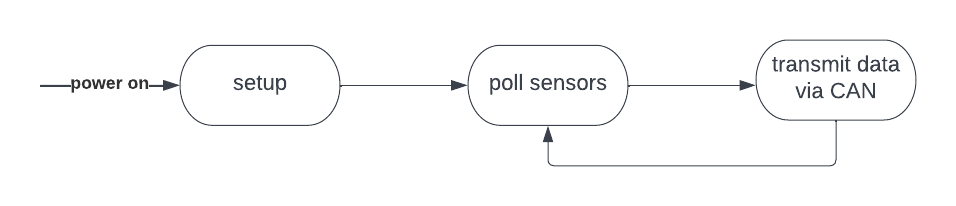
\includegraphics[width=7in]{images/sdm23software(1).png}
    \caption{State diagram for IMU and IO boxes}
    \label{fig:sdmioafsdasfs}
\end{figure}
\begin{figure}[H]
    \centering
    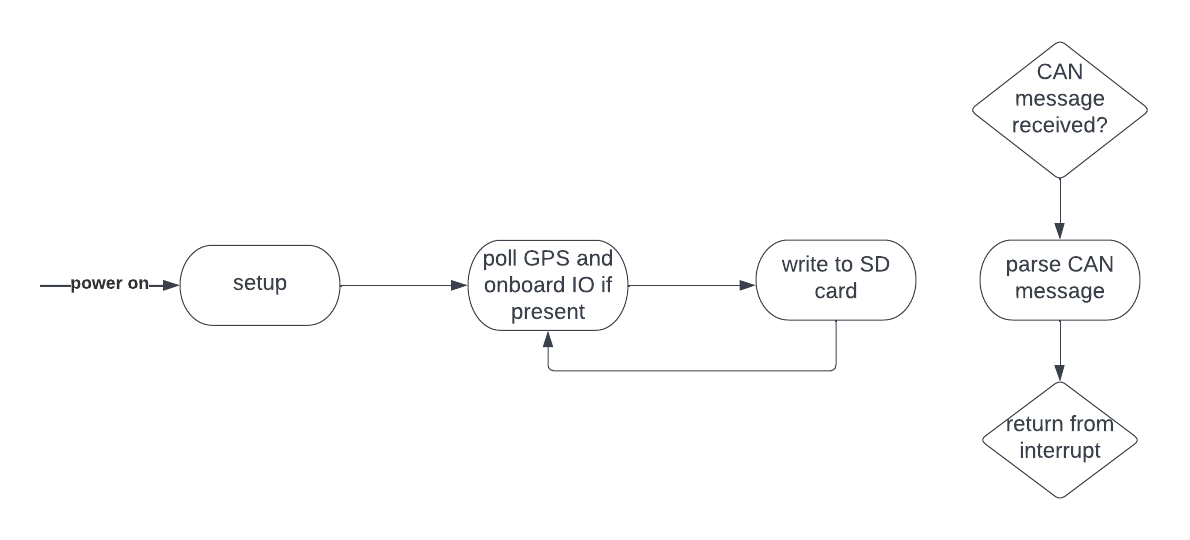
\includegraphics[width=7.5in]{images/ffff.png}
    \caption{State diagram for Main box}
    \label{fig:asdfasdfasdf}
\end{figure}
Figure \ref{fig:asdfasdfasdf} shows the state diagram for the Main box.
When the main box receives a CAN message, the SN65HVD230 triggers an interrupt for the Teensy software to parse the CAN message, returning to normal execution afterwards.
\vspace{1em}

For all boxes, once the setup function passes the onboard Teensy LED is lit up to indicate that everything has initialized successfully.

\section{Main Box Design}
The main box, using a Teensy 4.1 as its microcontroller, acts as a hub to collect data from the Haltech ECU, Front and Rear IO boxes and the IMU box via CAN.
\begin{figure}[H]
    \centering
    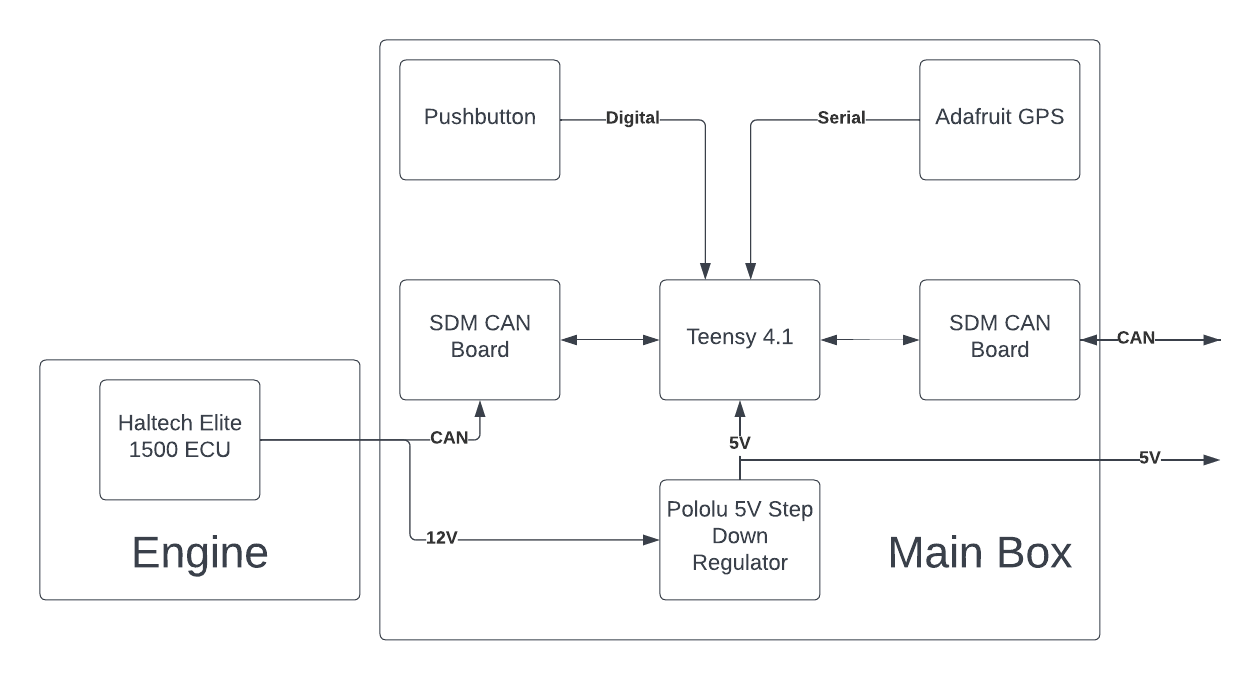
\includegraphics[width=5.5in]{images/SDM-23 Main Box Block Diagram.png}
    \caption{Main Box Block Diagram}
    \label{fig:sdm23mainboxblock}
\end{figure}

The main box includes an onboard GPS module to collect positional data and breakouts some extra I/O pins.
For data storage, the onboard Teensy 4.1's microSD card slot is used.
It receives 12V power from the ECU, which is stepped down to 5V using a Pololu 5V regulator.
The 5V is then passed to the onboard Teensy 4.1 as well as to any DAQ component connected to the main box.
It also includes a pushbutton which can be used to mark notable timestamps in order to sync with other systems (e.g., Go Pros).
\vspace{1em}

The main box also includes a panel mount micro USB connector which is connected to the Teensy 4.1's micro USB port, which will allow us to easily debug and reprogram the Teensy 4.1, and also to retrieve the data via USB.
This will greatly decrease the time and effort needed to debug the box or retrieve data, since it will no longer be necessary to disassemble the box in order to do either of the aforementioned tasks.
\vspace{1em}

The main constraint for the main box's PCB design was that it should fit within a 100mm x 100mm square, which is JLCPCB's cheapest tier for PCB manufacturing.
To cut down on assembly cost and design time, custom SN65HVD230 breakout boards were used to complete the electrical interface between the Teensy 4.1 and the CAN bus as opposed to laying out the CAN transceiver circuitry on the main board directly.
The design for the custom SN65HVD230 breakout board is detailed in Section \ref{sec:canboard}.
\vspace{1em}

The Teensy 4.1 requires $V_{in}$ to be between 3.6 and 5.5V.
However, the Haltech ECU's CAN Hub supplies 12V power.
Although the ECU is also capable of supplying 5V, upon testing of SDM-21.5 it was discovered that the DAQ electrical system requires more current than what the ECU can output on 5V.
As such, we needed a method of stepping down 12V into an acceptable level to power the Teensy 4.1.
We selected Pololu's 5V, 2.5A Step-Down Voltage Regulator to provide the Teensy 4.1 (as well as the rest of the DAQ electrical system) 5V.
By using this regulator, we were able to save time and manufacturing costs by not having to design our own voltage regulator circuitry.
\vspace{1em}

It was also decided to break out unused pins of the Teensy 4.1.
These would come in useful as we were able to connect a damper potentiometer directly to the main box during testing.
\begin{figure}[H]
    \centering
    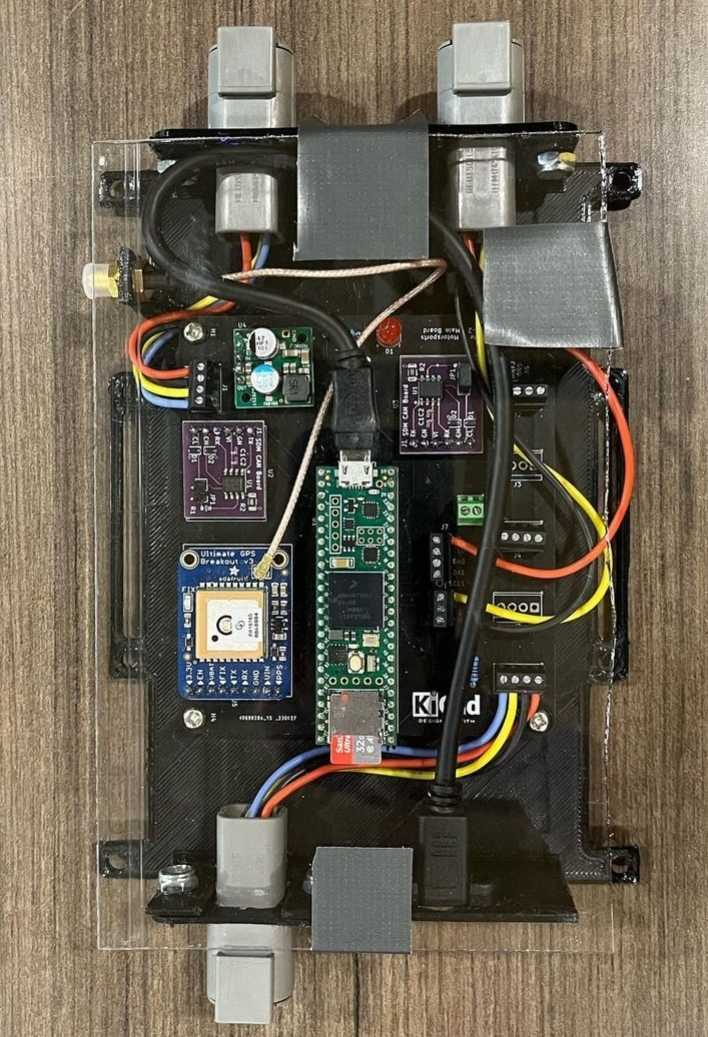
\includegraphics[width=3in,angle=90]{images/main.jpg}
    \caption{Main Box plate with assembled electronics}
    \label{fig:sdm23mainbox}
\end{figure}
\begin{figure}[H]
    \centering
    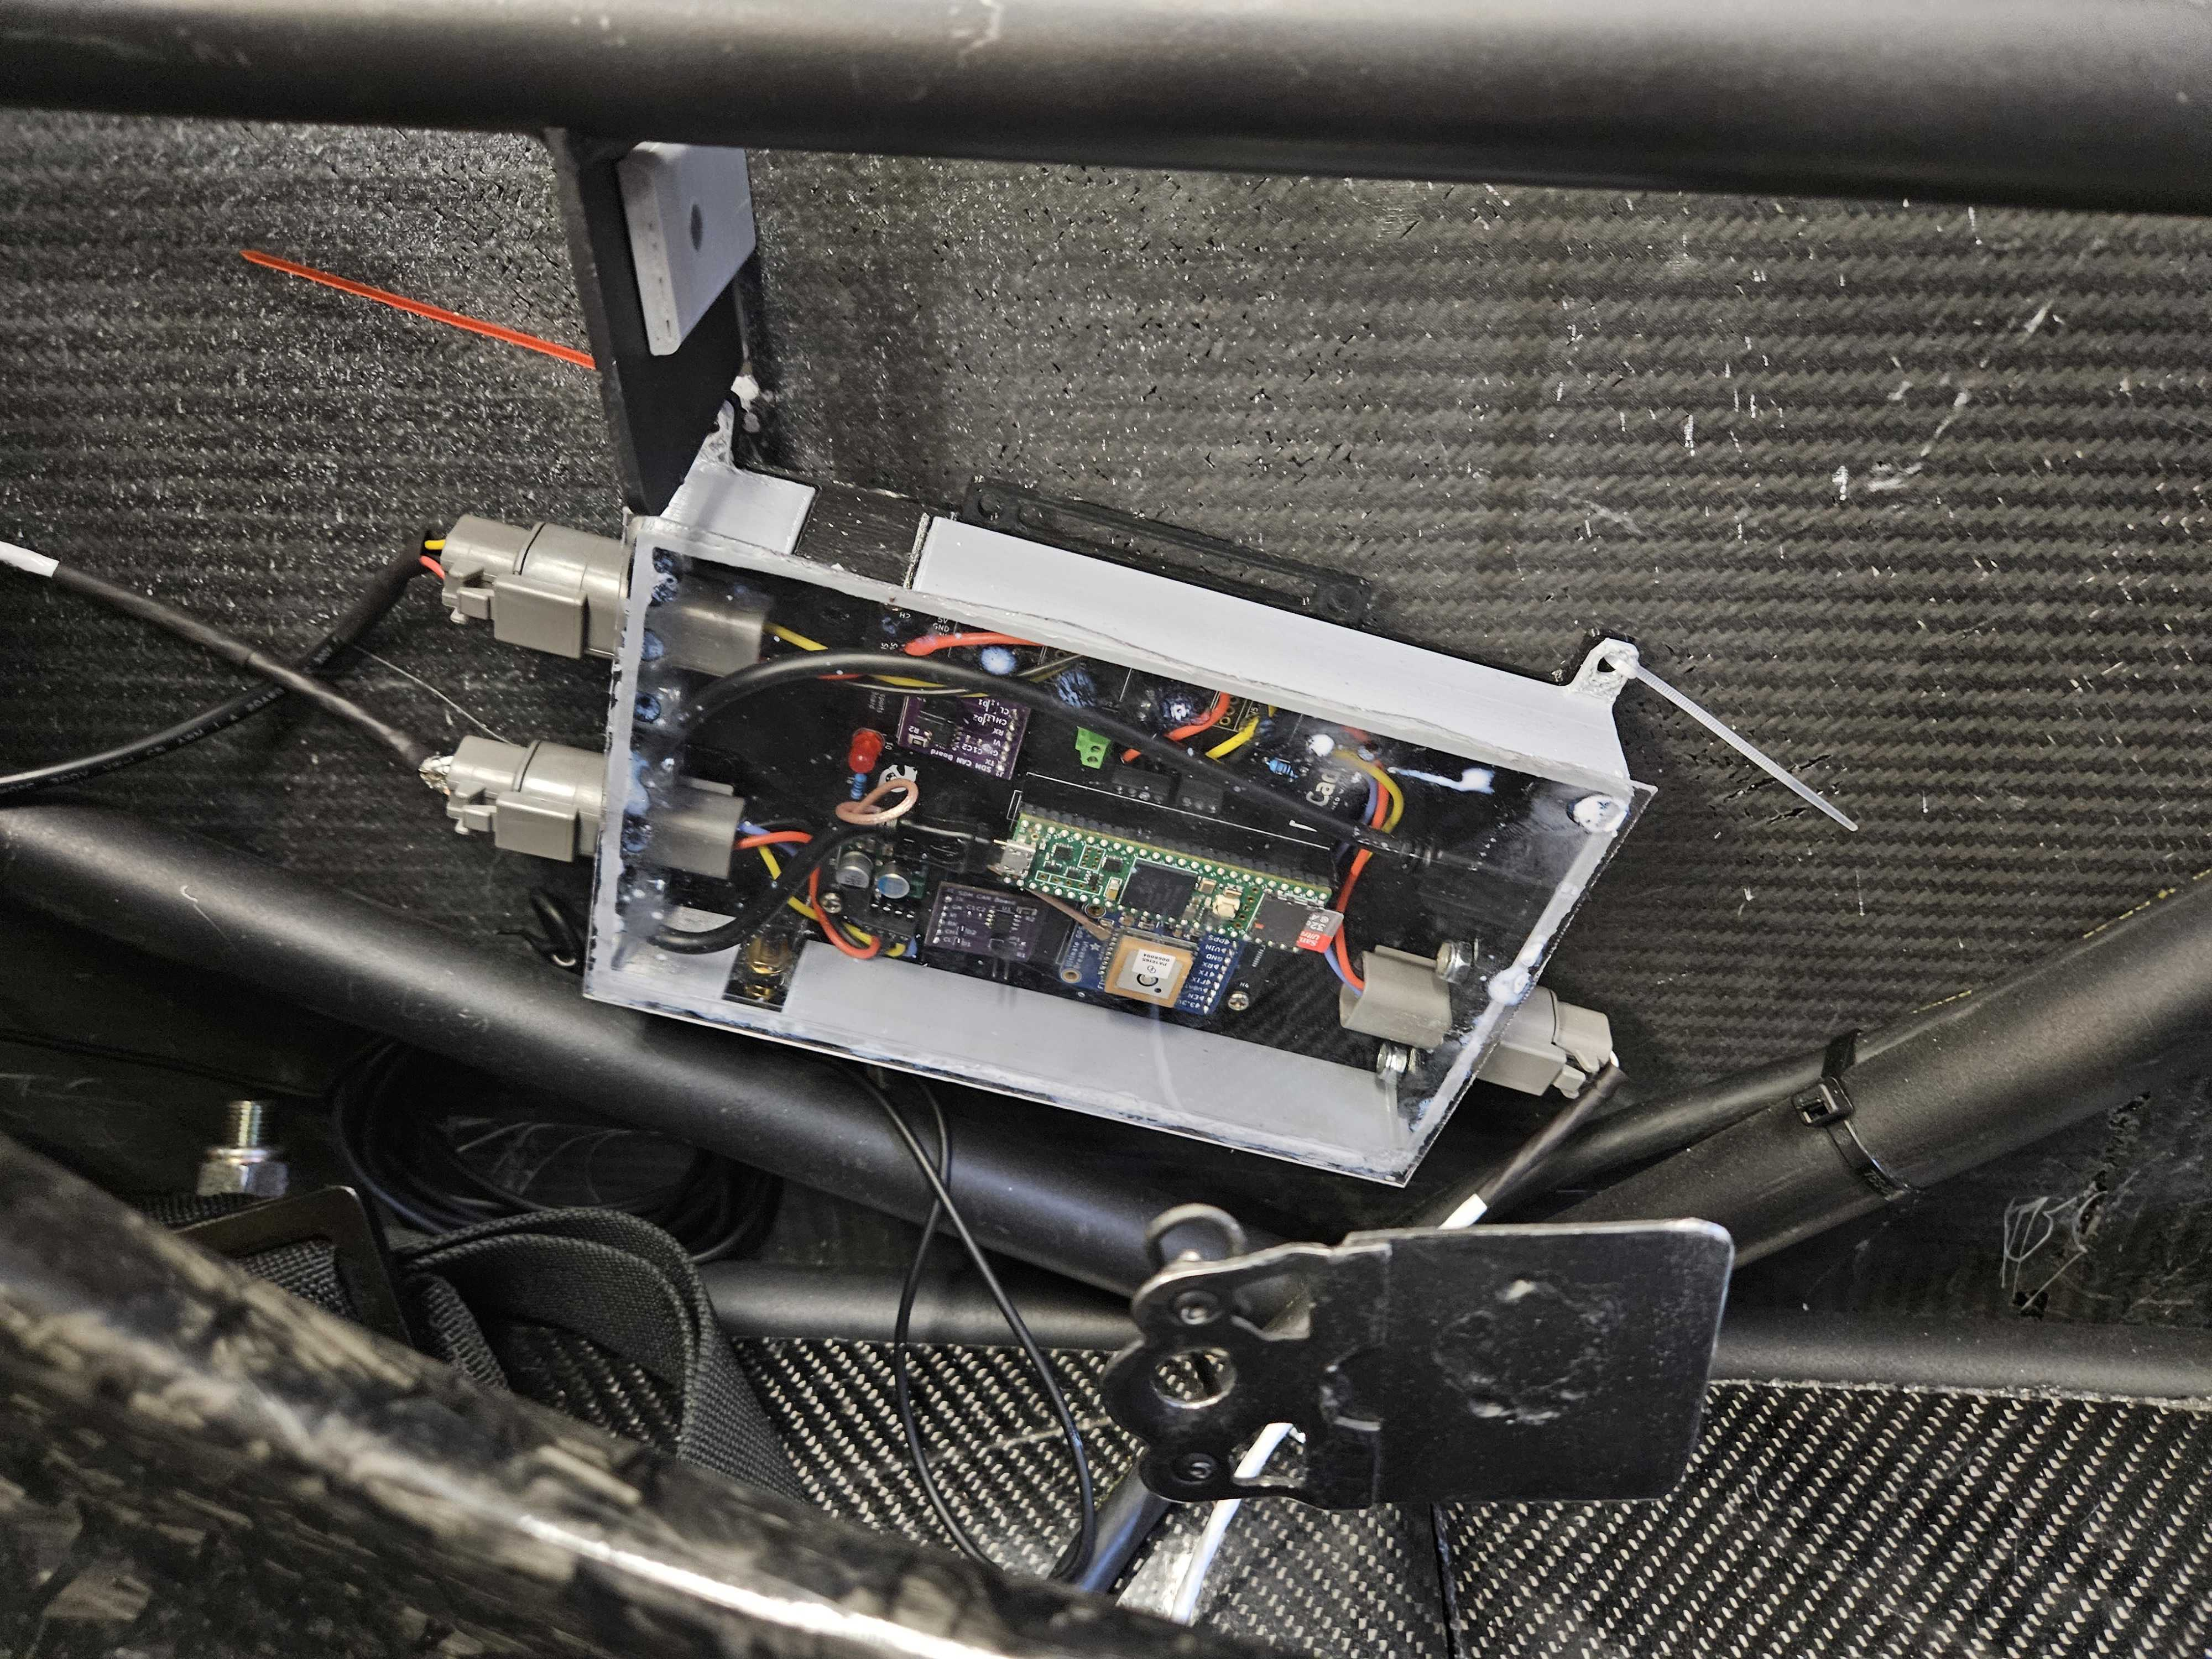
\includegraphics[width=5in]{images/asdf.jpg}
    \caption{Installed Main box in cockpit}
    \label{fig:main}
\end{figure}
The enclosure for the Main box consists of a plate that the PCB and connector panels are screwed into, a gasket, and a polycarbonate cover.
Both the plate and the gasket were 3D-printed.


\section{IMU Box Design}
The IMU box's purpose is to collect data from the ISM330DHCX and relay it to the main box via CAN.
Since the IMU box needed to be as small as possible and there was no need for onboard data storage, a Teensy 4.0 was selected to be its microcontroller.
\begin{figure}[H]
    \centering
    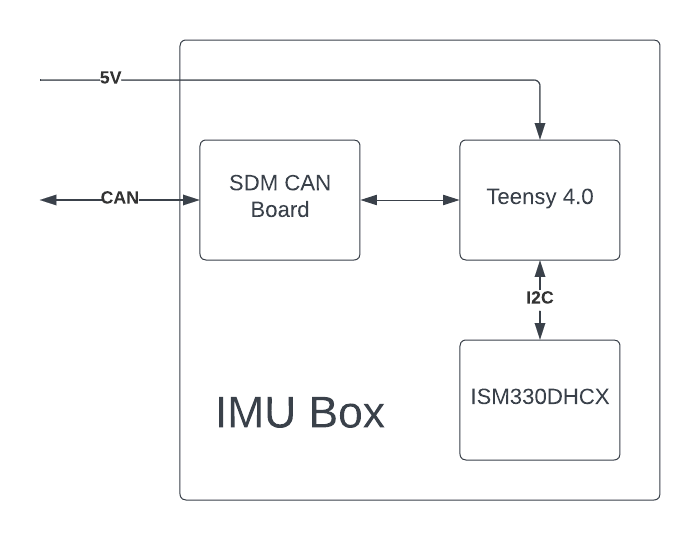
\includegraphics[width=4in]{images/SDM-23 IMU Box Block Diagram .png}
    \caption{IMU Box Block Diagram}
    \label{fig:sdm23imuboxblock}
\end{figure}
We opted to use Sparkfun's ISM330DHCX breakout board for the IMU board because we determined that it was a safer option rather than designing the IMU circuitry ourselves because we would be able to easily swap out the IMU in case it became damaged or nonfunctional for whatever reason.
\vspace{1em}

Since the IMU box was likely to be placed somewhere in the center of the car, the IMU box's pinout included a second CAN connection with 5V and GND so that we would be able to daisy chain the CAN bus, meaning that the stub length for the IMU is completely minimized.
This was able to be utilised, as the IMU box was placed underneath the driver seat and we were able to route the CAN bus from the Main box, to the IMU box, and then to the Front I/O box.
\vspace{1em}

Like the Main box, the enclosure for the IMU box consists of a 3D-printed plate and gasket and a polycarbonate cover.
\begin{figure}[H]
    \centering
    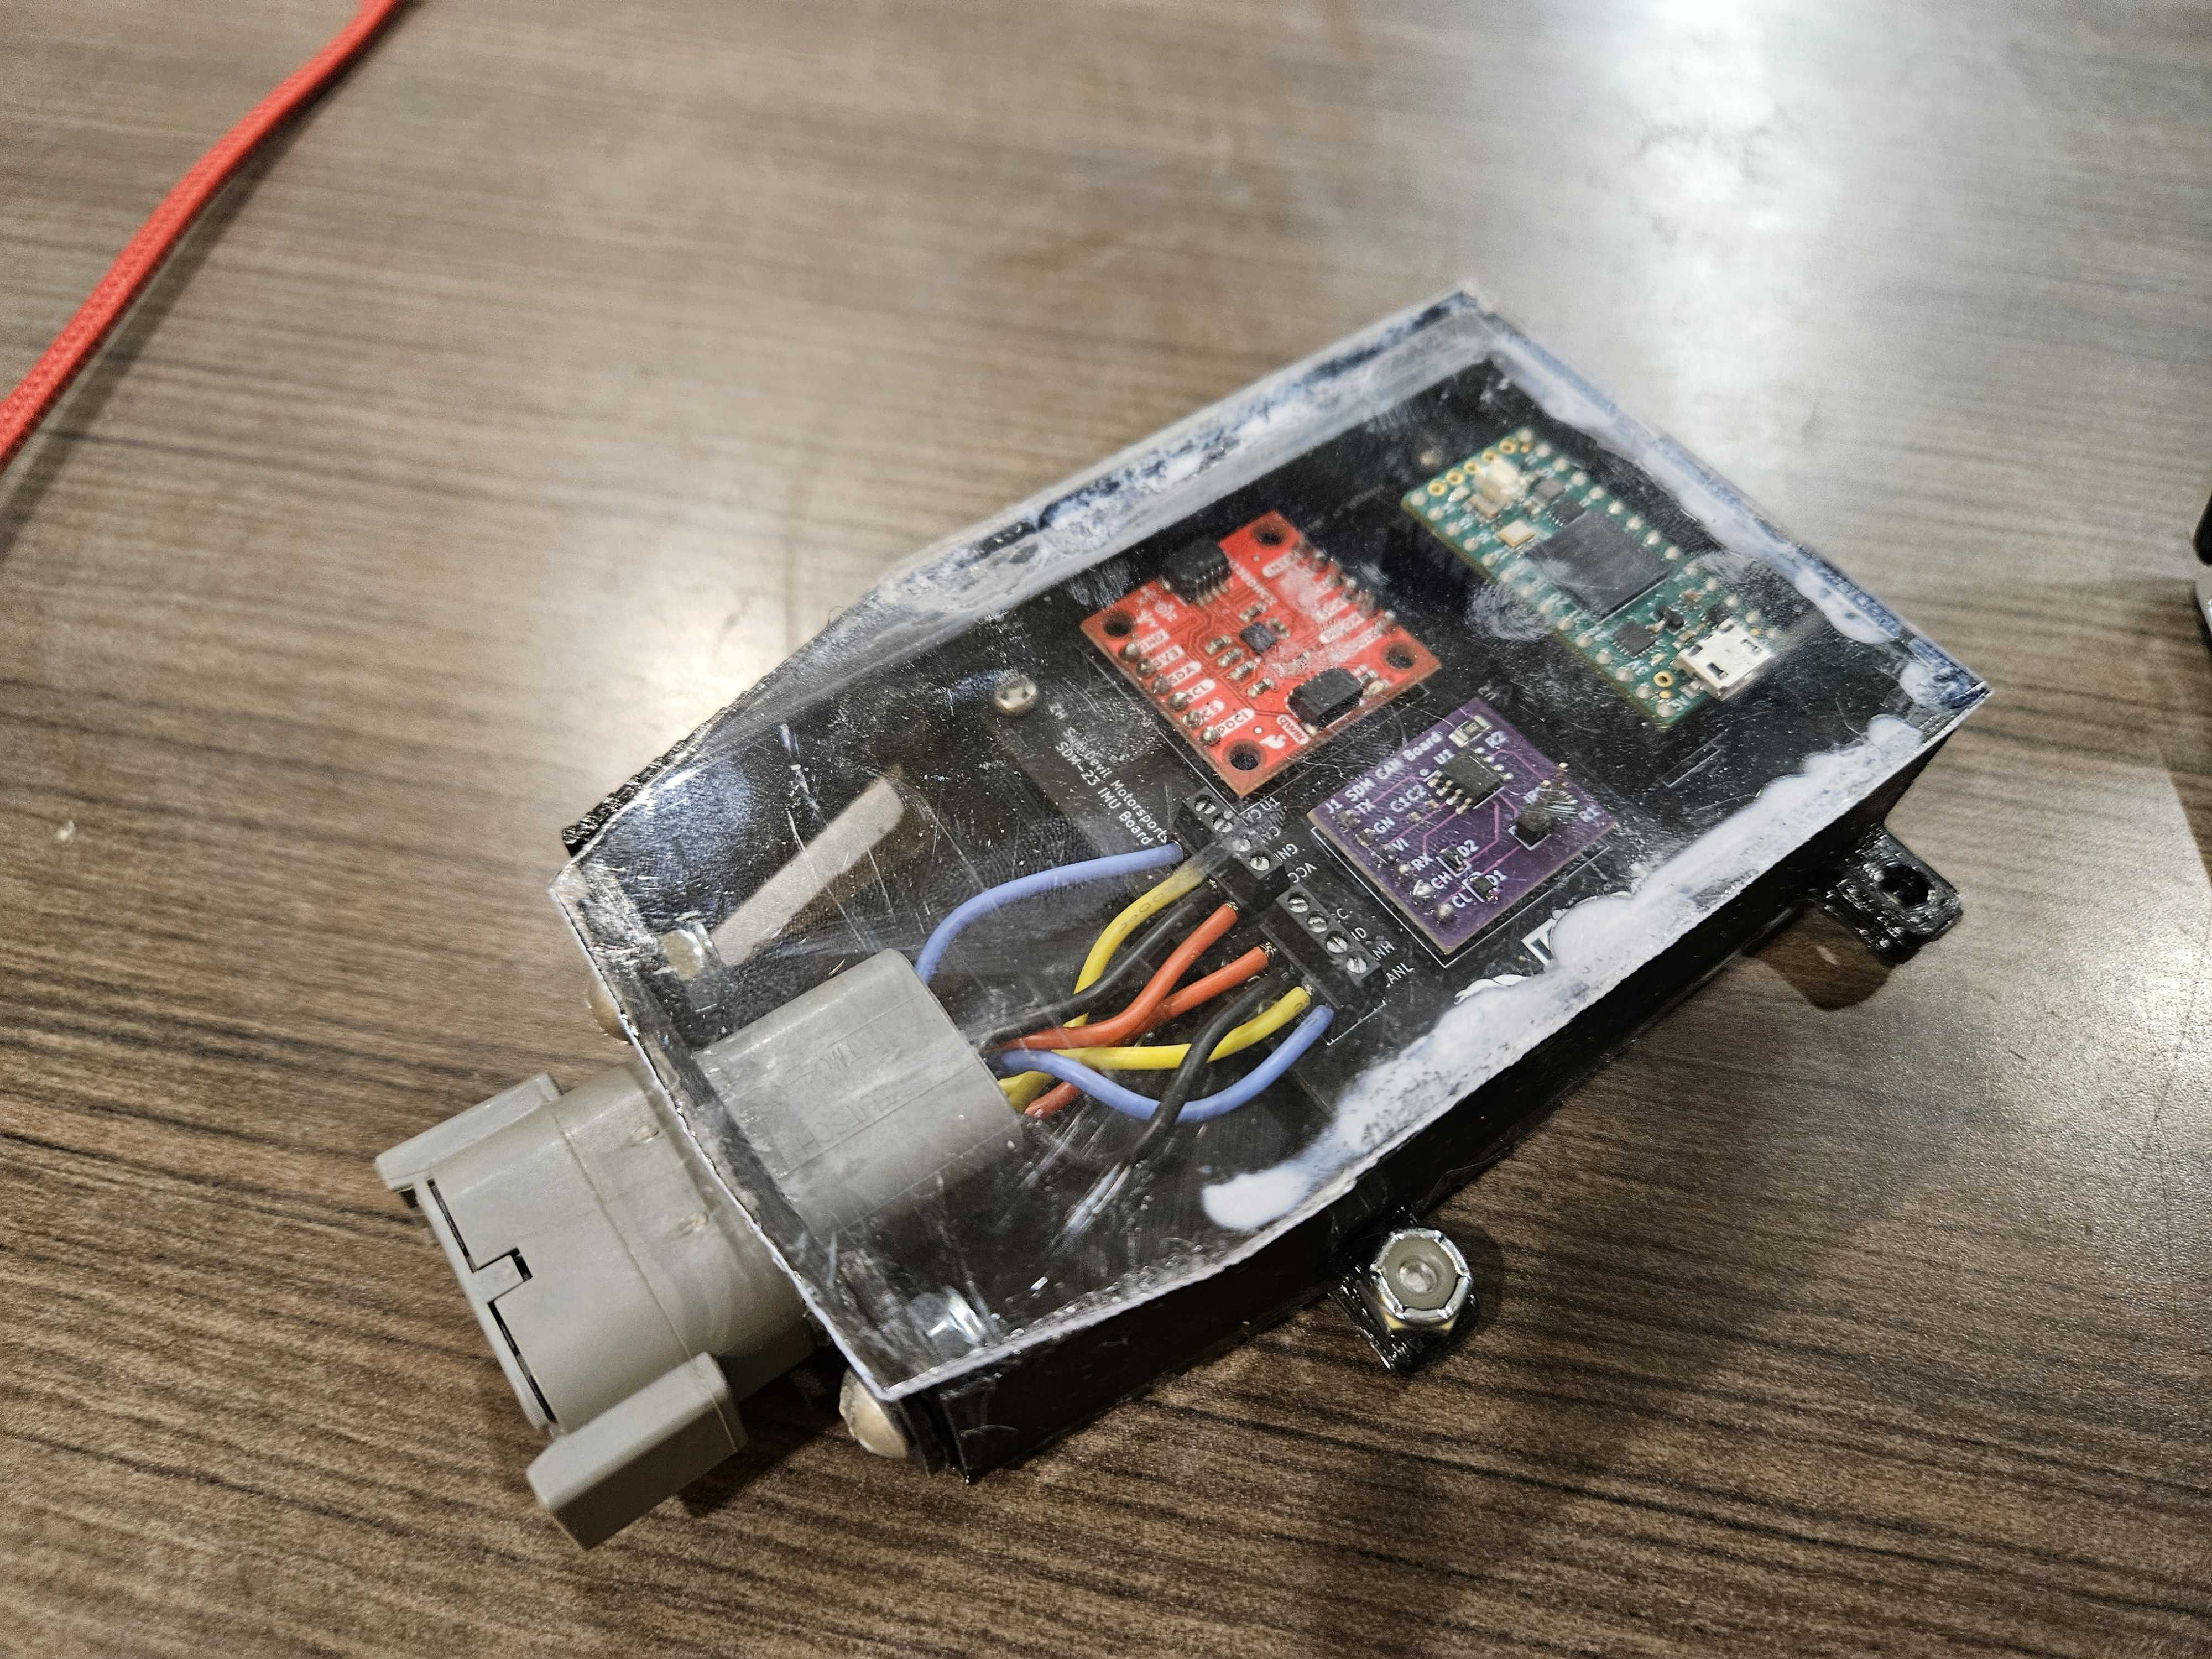
\includegraphics[width=4in]{images/imuimu.jpg}
    \caption{Assembled IMU box}
    \label{fig:sdm23imubox}
\end{figure}
\subsection{Gyroscope Debugger}
To assist in tuning the gyroscope to produce as clean data as possible, a debugging software was developed to plot and integrate the angular rate produced by the gyroscope.
It works by the Teensy 4.0 relaying gyroscope data to a computer via USB Serial.
The debugger then parses the data and plots it using \texttt{pyqtgraph}.
The software also gives the option for the user to input a zero value to use for integration, and includes a model of SDM-23 to visualize the car's angular position.
\begin{figure}[H]
    \centering
    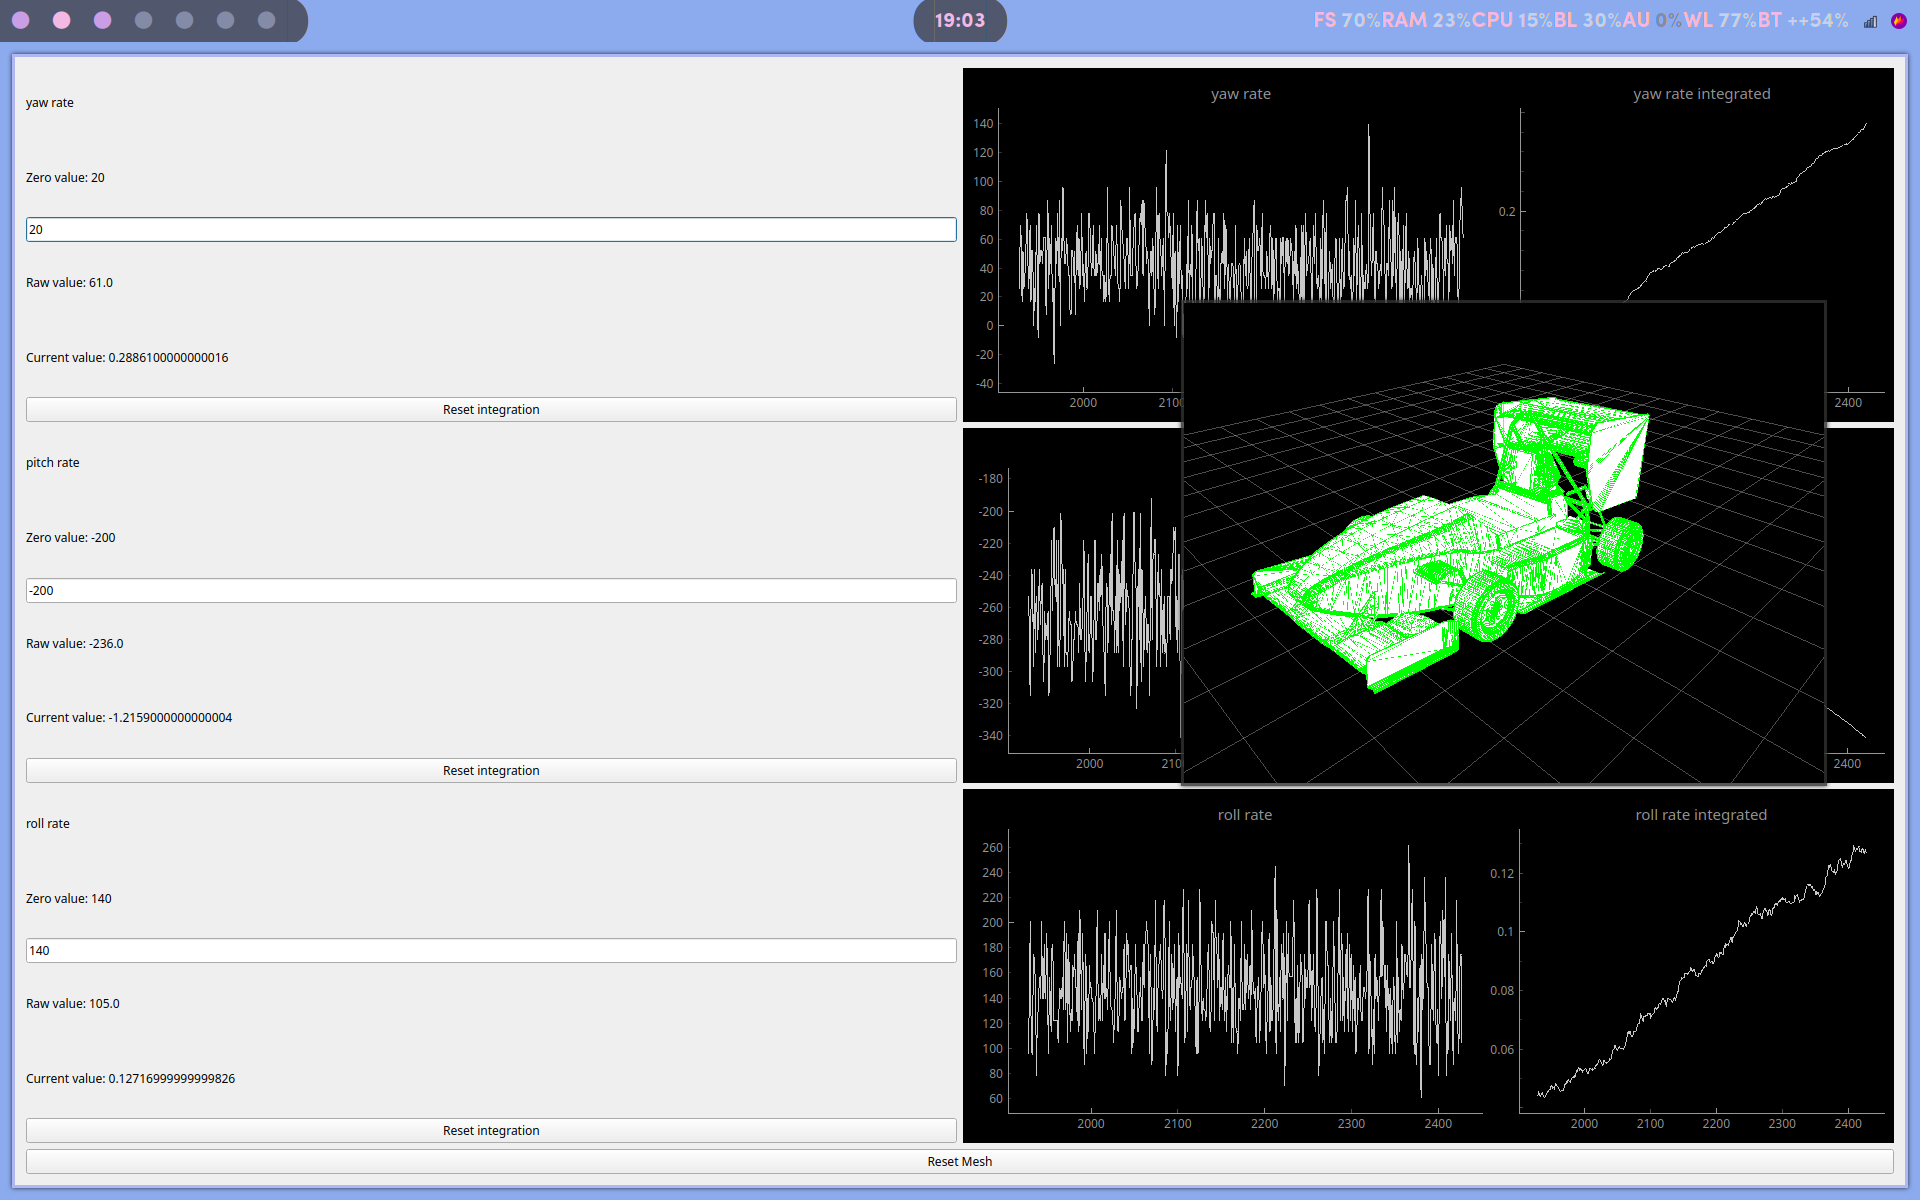
\includegraphics[width=7in]{images/debug.png}
    \caption{Gyroscope debugger software}
    \label{fig:deb}
\end{figure}

\section{Front/Rear IO Box Design}
The I/O Boxes are responsible for interfacing with the majority of SDM-23's sensors.
Its primary components are a Teensy 4.0 and a CAN transceiver board.
\begin{figure}
    \centering
    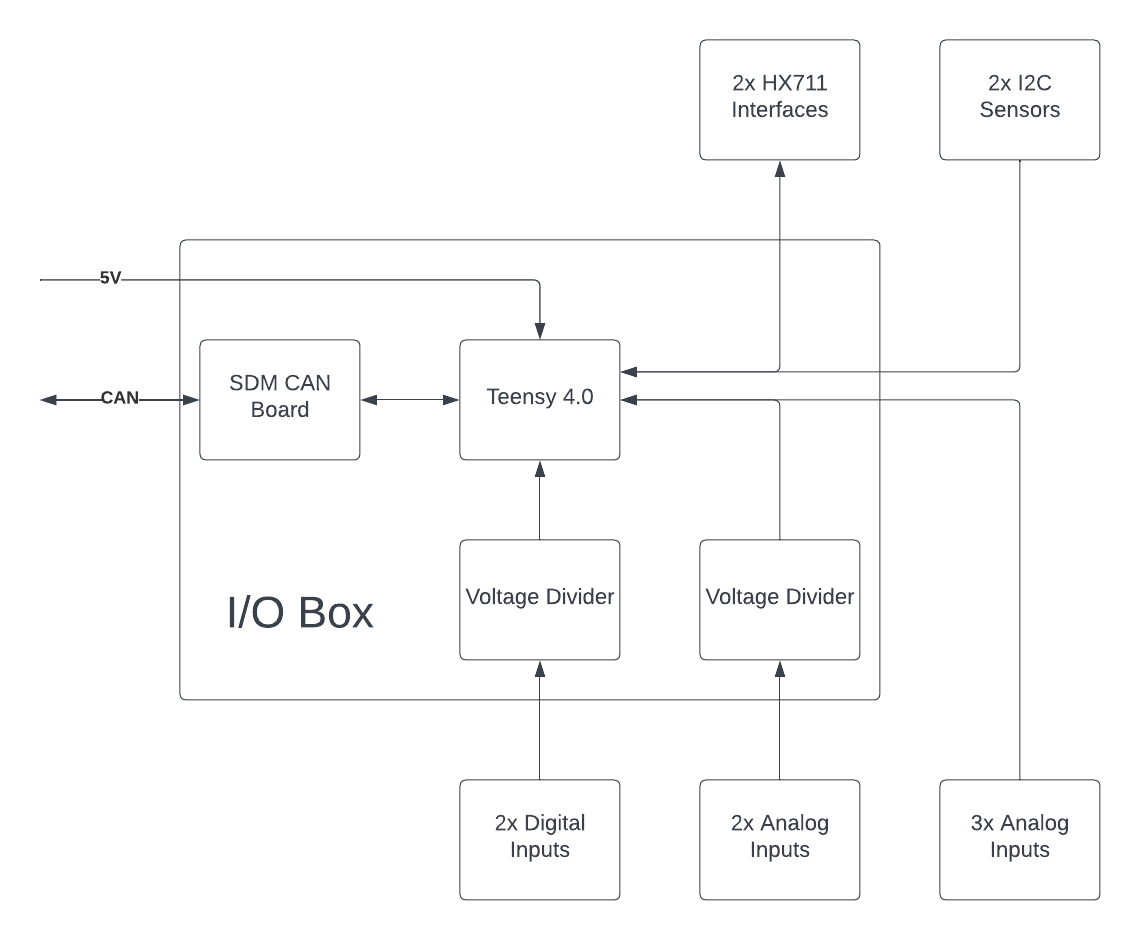
\includegraphics[width=5in]{images/SDM-23 IO Box Block Diagram.png}
    \caption{I/O Box Block Diagram}
    \label{fig:sdm23ioboxblock}
\end{figure}
It includes pinouts for:
\begin{itemize}
    \item 2x 5V digital inputs
    \item 2x 5V analog inputs
    \item 3x 3.3V analog inputs
    \item 2x 3.3V I2C sensors
    \item 2x HX711 interfaces
\end{itemize}
It was designed to be agnostic enough where it can be used in any car produced by the team.
For SDM-23, the Front I/O makes use of both HX711 interfaces, both 5V analog inputs for the brake pressure sensors, one I2C sensor for the brake temperature sensor, and one 3.3V analog input for the steering angle sensor.
\vspace{1em}

The box has one DTM-4 connector for the CAN connection, and 3 DTM-12 connectors, where one connector would be for sensors on the front left side of the car, one would be for sensors on the front right side, and one would be for other sensors.

\begin{figure}
    \centering
    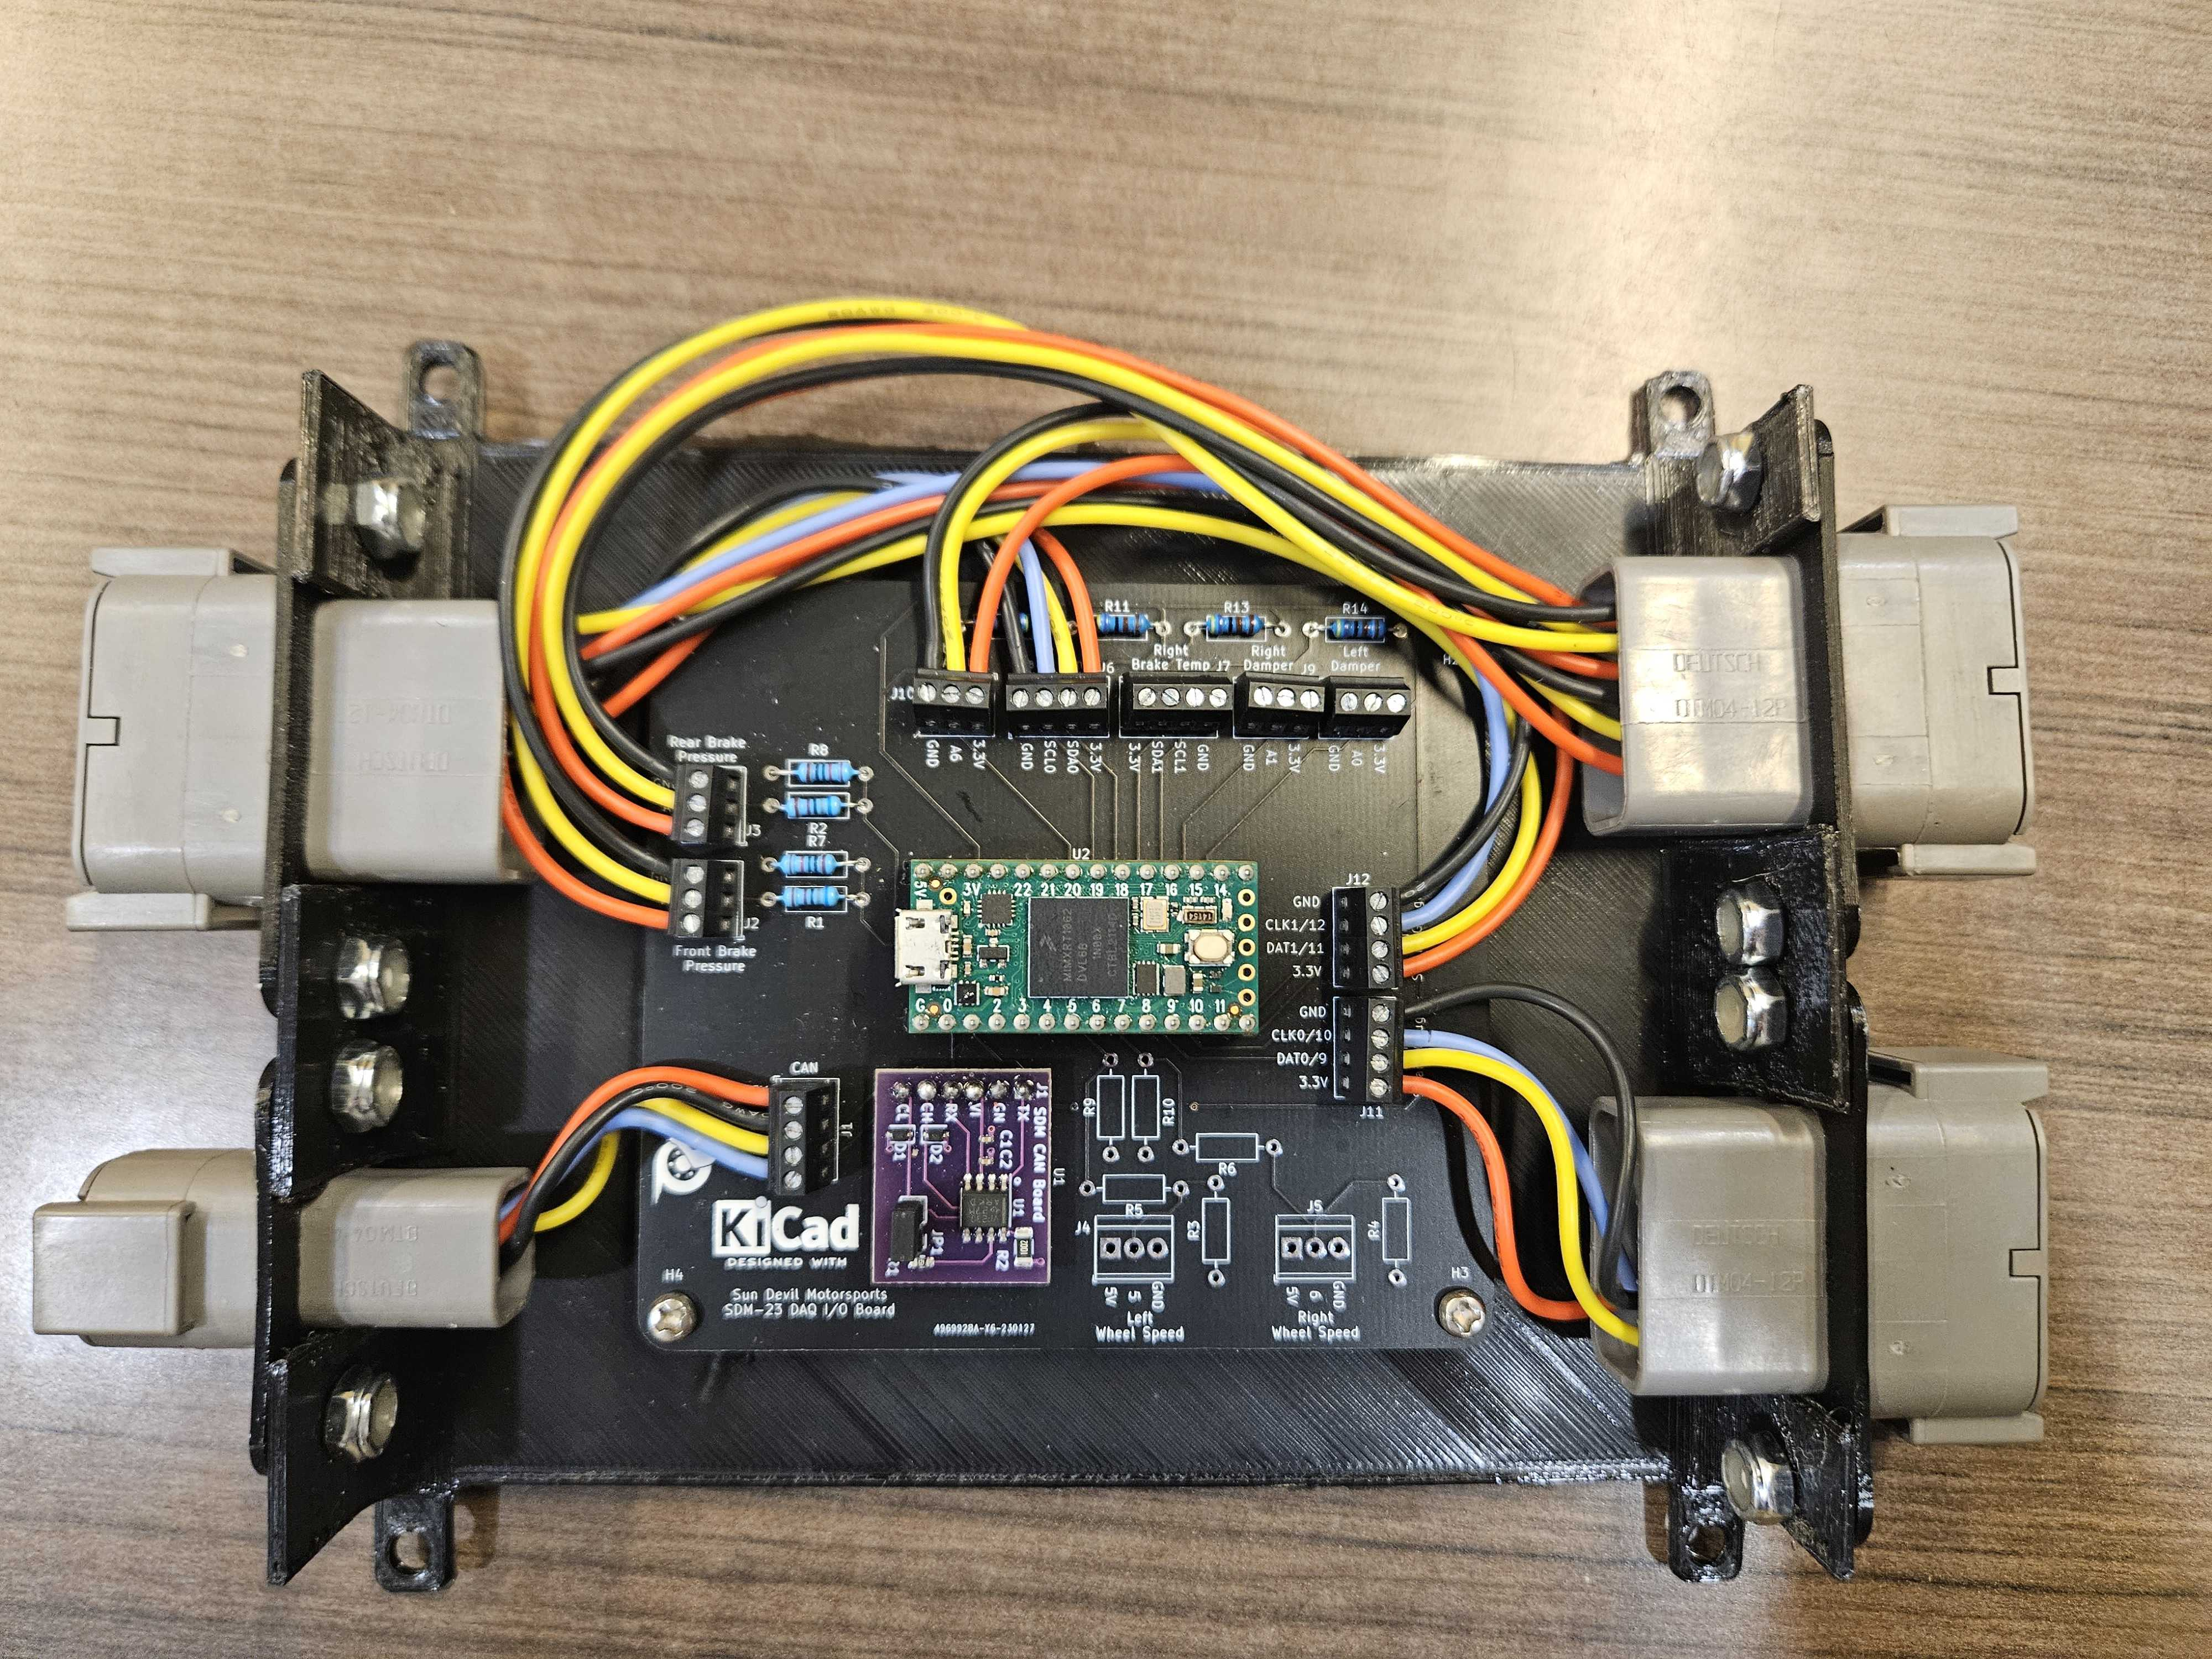
\includegraphics[width=5in]{images/io.jpg}
    \caption{IO Box plate with assembled electronics for front I/O}
    \label{fig:io}
\end{figure}

2.7k$\Omega$ Pull-up resistors for the I2C sensors are built-in to the PCB, and the voltage dividers use 6.8k$\Omega$ and 10k$\Omega$ resistors for $R_1$ and $R_2$ respectively to step down 5V into a 3V range.



\section{CAN Transceiver Board Design}\label{sec:canboard}
The CAN transceiver board provides a pinout for the SN65HVD230 CAN transceiver.
Since virtually all of the boards designed for this package requires a CAN transceiver and its supporting circuitry, a breakout board was designed so that we would design the circuitry once and be able to implement it on all of the boards in the package.
This would also allow us to test and prototype circuitry for the DAQ package on breadboards before the PCB designs were manufactured.
\vspace{1em}

A custom breakout board was designed as opposed to purchasing a commercial off-the-shelf solution because many boards available for purchase had a $120\Omega$ resistor soldered directly, meaning that if a node wasn't supposed to be terminating the resistor had to be completely desoldered.
So a design goal for this board was to include optional termination, where a jumper could be added if the resistor needed to be used.
\vspace{1em}

The SN65HVD230 comes with integrated slope control, which adjusts the output rise and fall slopes.
If the $R_S$ pin is strongly pulled to ground it is in high speed mode, where the output is allowed to switch as fast as possible.
If a $10k\Omega$ to $100k\Omega$ resistor is connected between $R_S$ and ground, then it is in slope control, where the output's slope is controlled and does not switch as fast.
This reduces the electromagnetic interference produced by the rise and fall times of the driver and resulting harmonics.
For this reason it was chosen to put the SN65HVD230 in slope control by connecting a $10k\Omega$ resistor between $R_S$ and ground.
\vspace{1em}

The rest of the supporting circuitry on the board such as bypass capacitors and ESD protection was guided by Texas Instruments' layout guidelines found in the SN65HVD230's datasheet.

\begin{figure}[H]
    \centering
    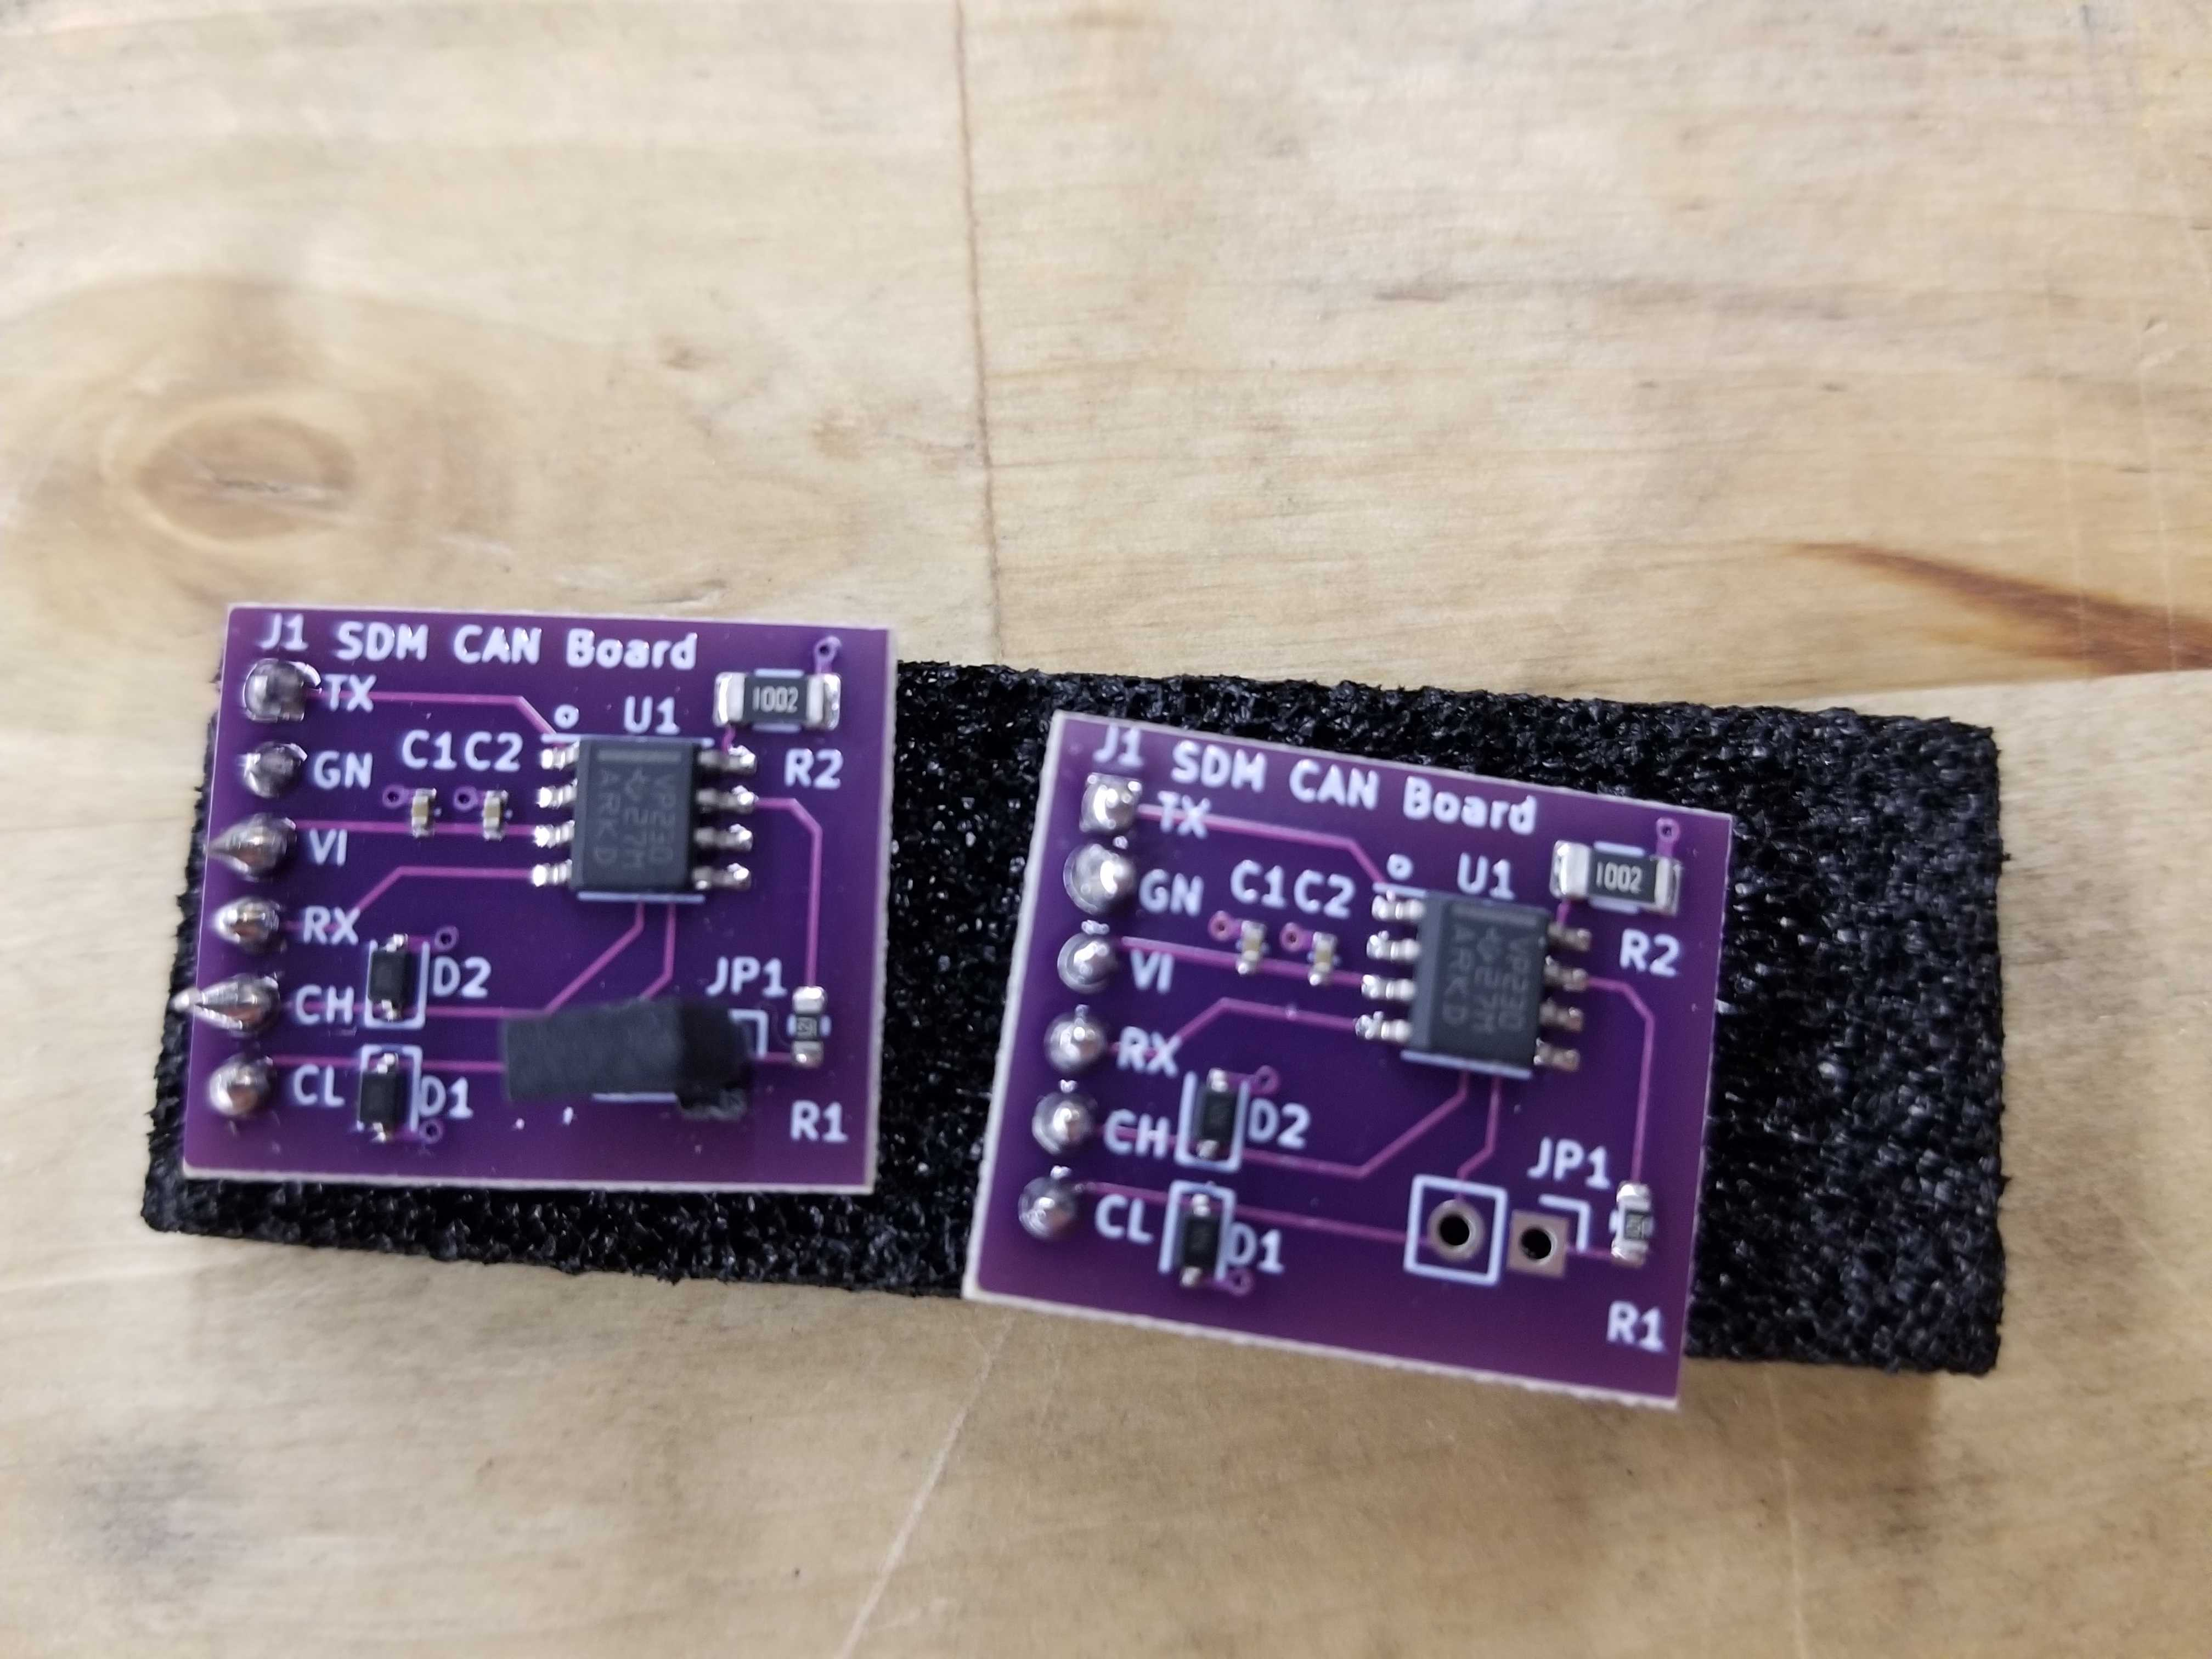
\includegraphics[width=4in]{images/sdmcanboardv1.jpg}
    \caption{CAN Transceiver Board}
    \label{fig:sdmcanboard}
\end{figure}


\section{Damper Potentiometer Design}
Linear potentiometers are used to measure the dampers' displacement and speed.
The design for the damper potentiometer consists of aluminum brackets, 3D-printed body and slide, and the linear potentiometer itself.
The 3D-printed portions of the design are mostly carried over from SDM-22, with the exception of the mounting holes and the filament used.
Instead of mounting the 3D-printed parts directly to the damper, these parts would be attached to aluminum brackets, which would attach to the damper.
In doing so, large spacers would not required to mount the potentiometer.
\begin{figure}[H]
    \centering
    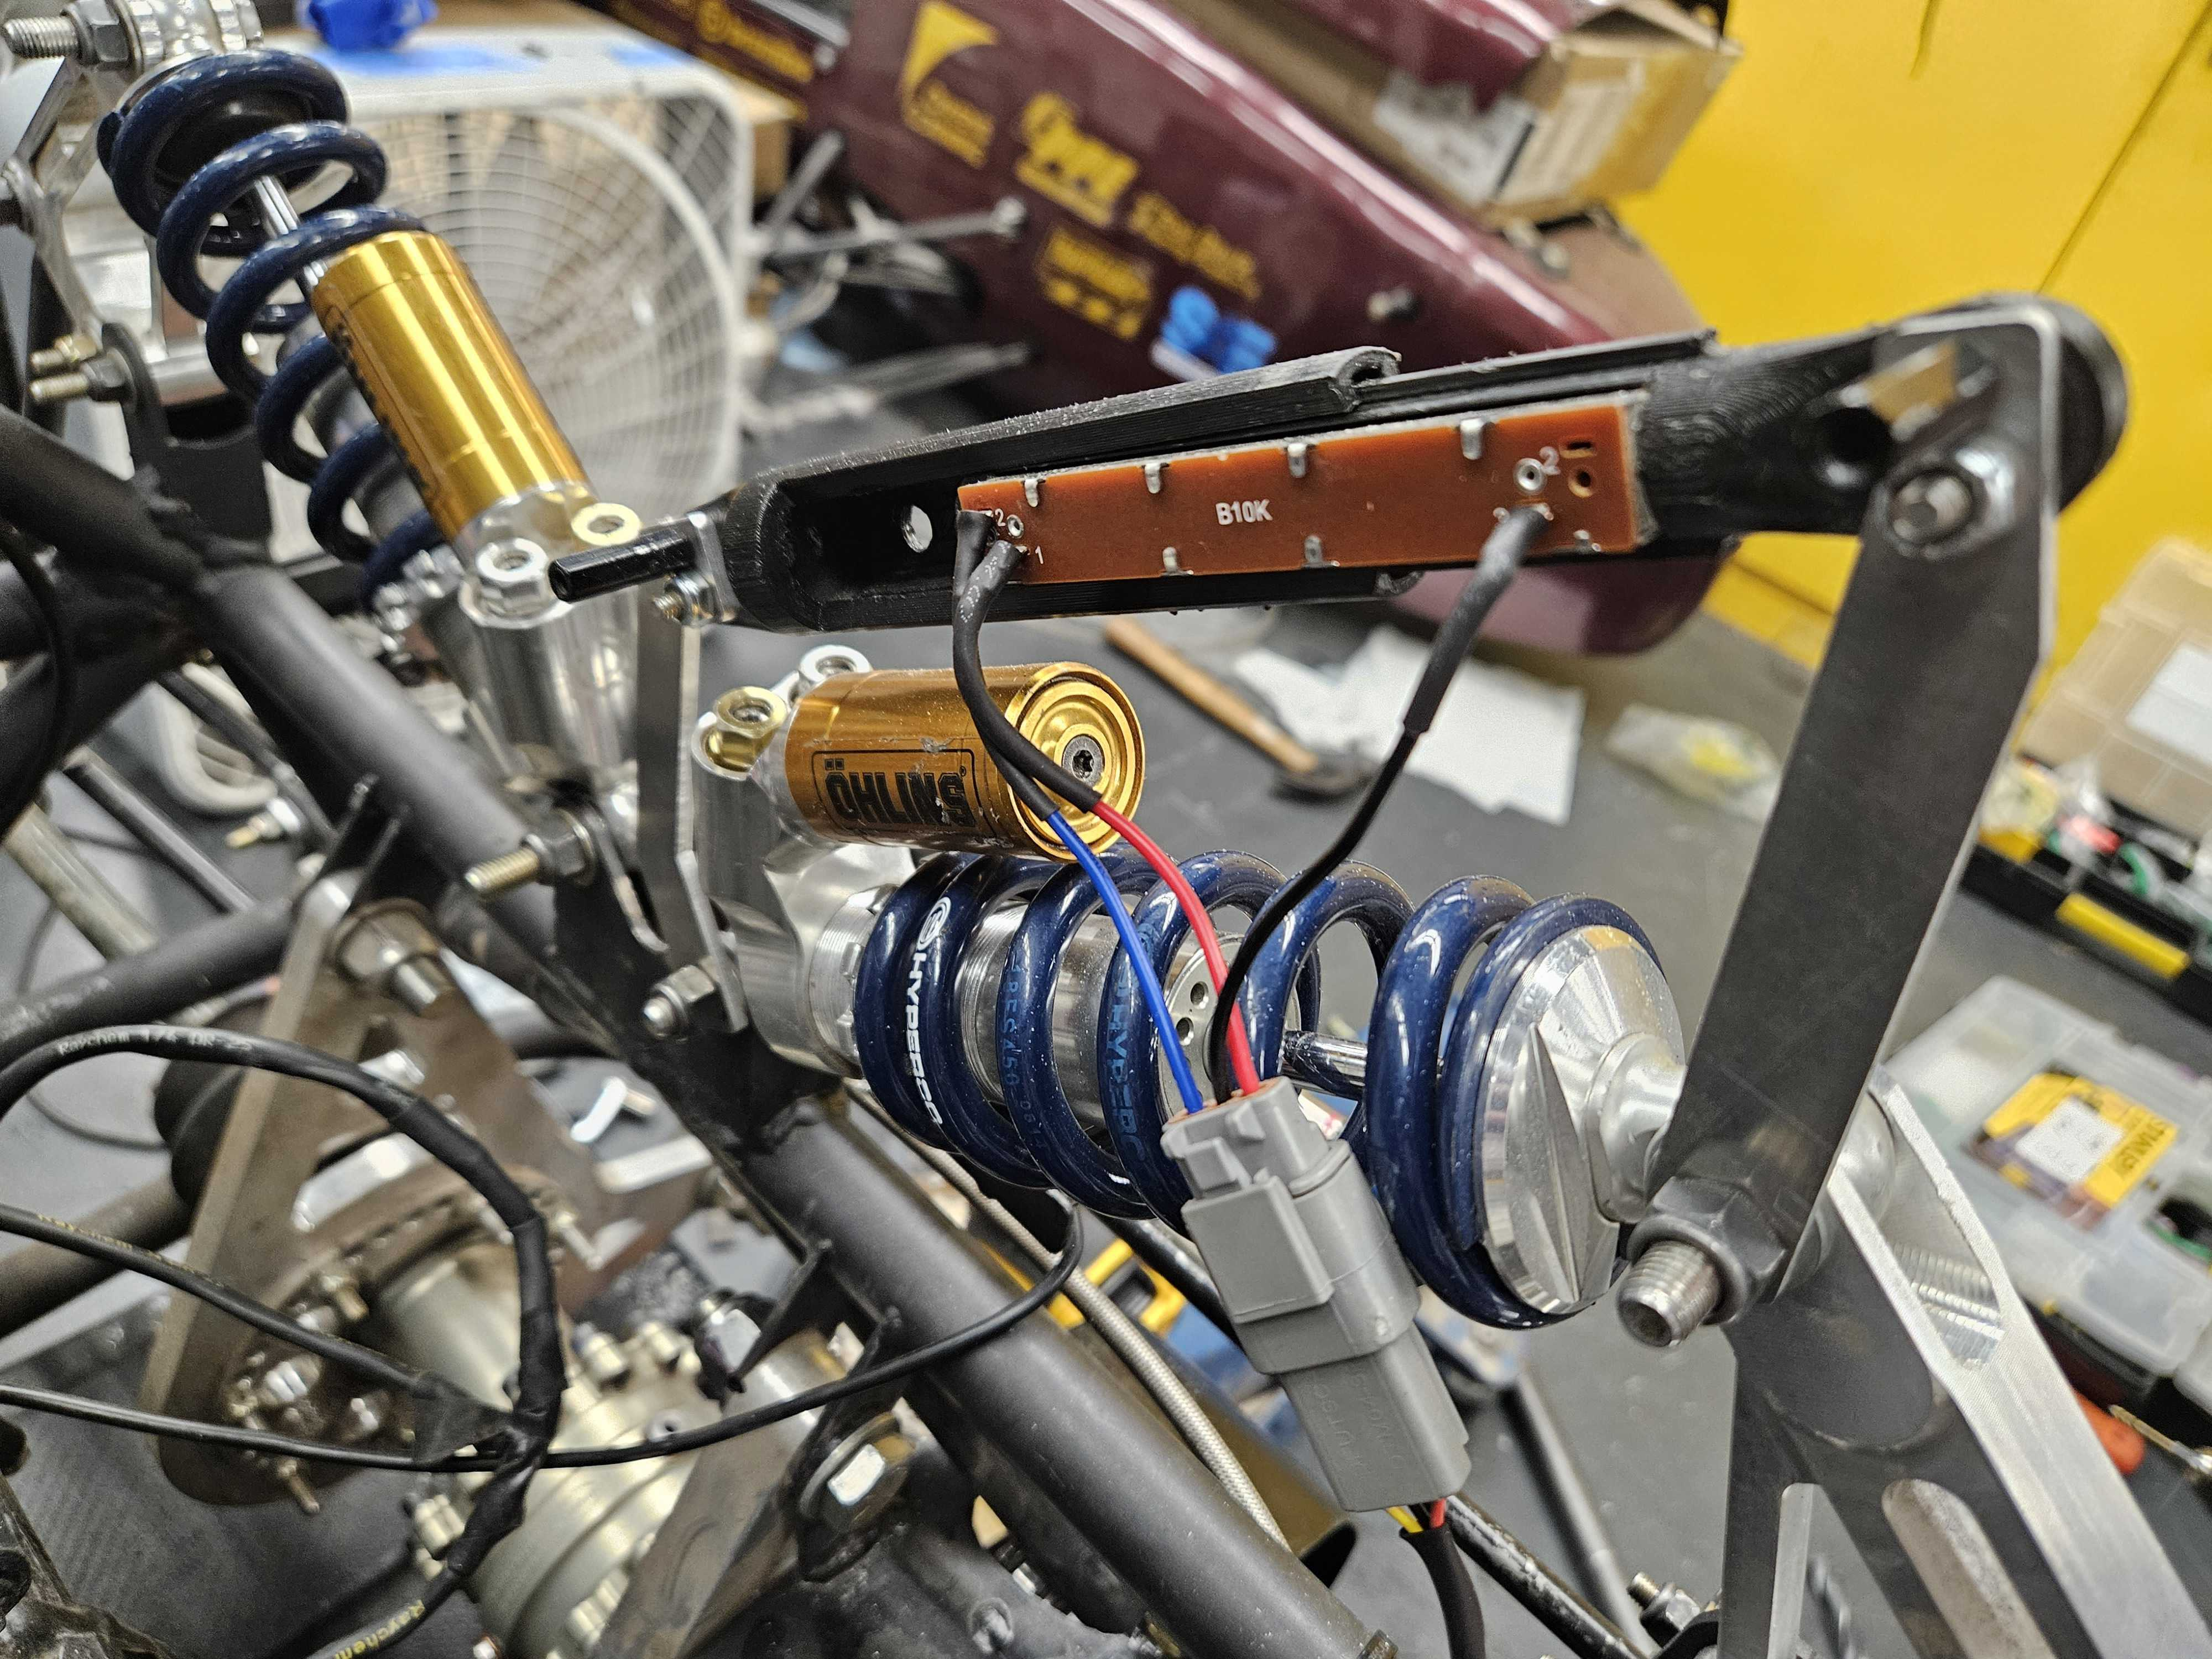
\includegraphics[width=3in]{images/pots.jpg}
    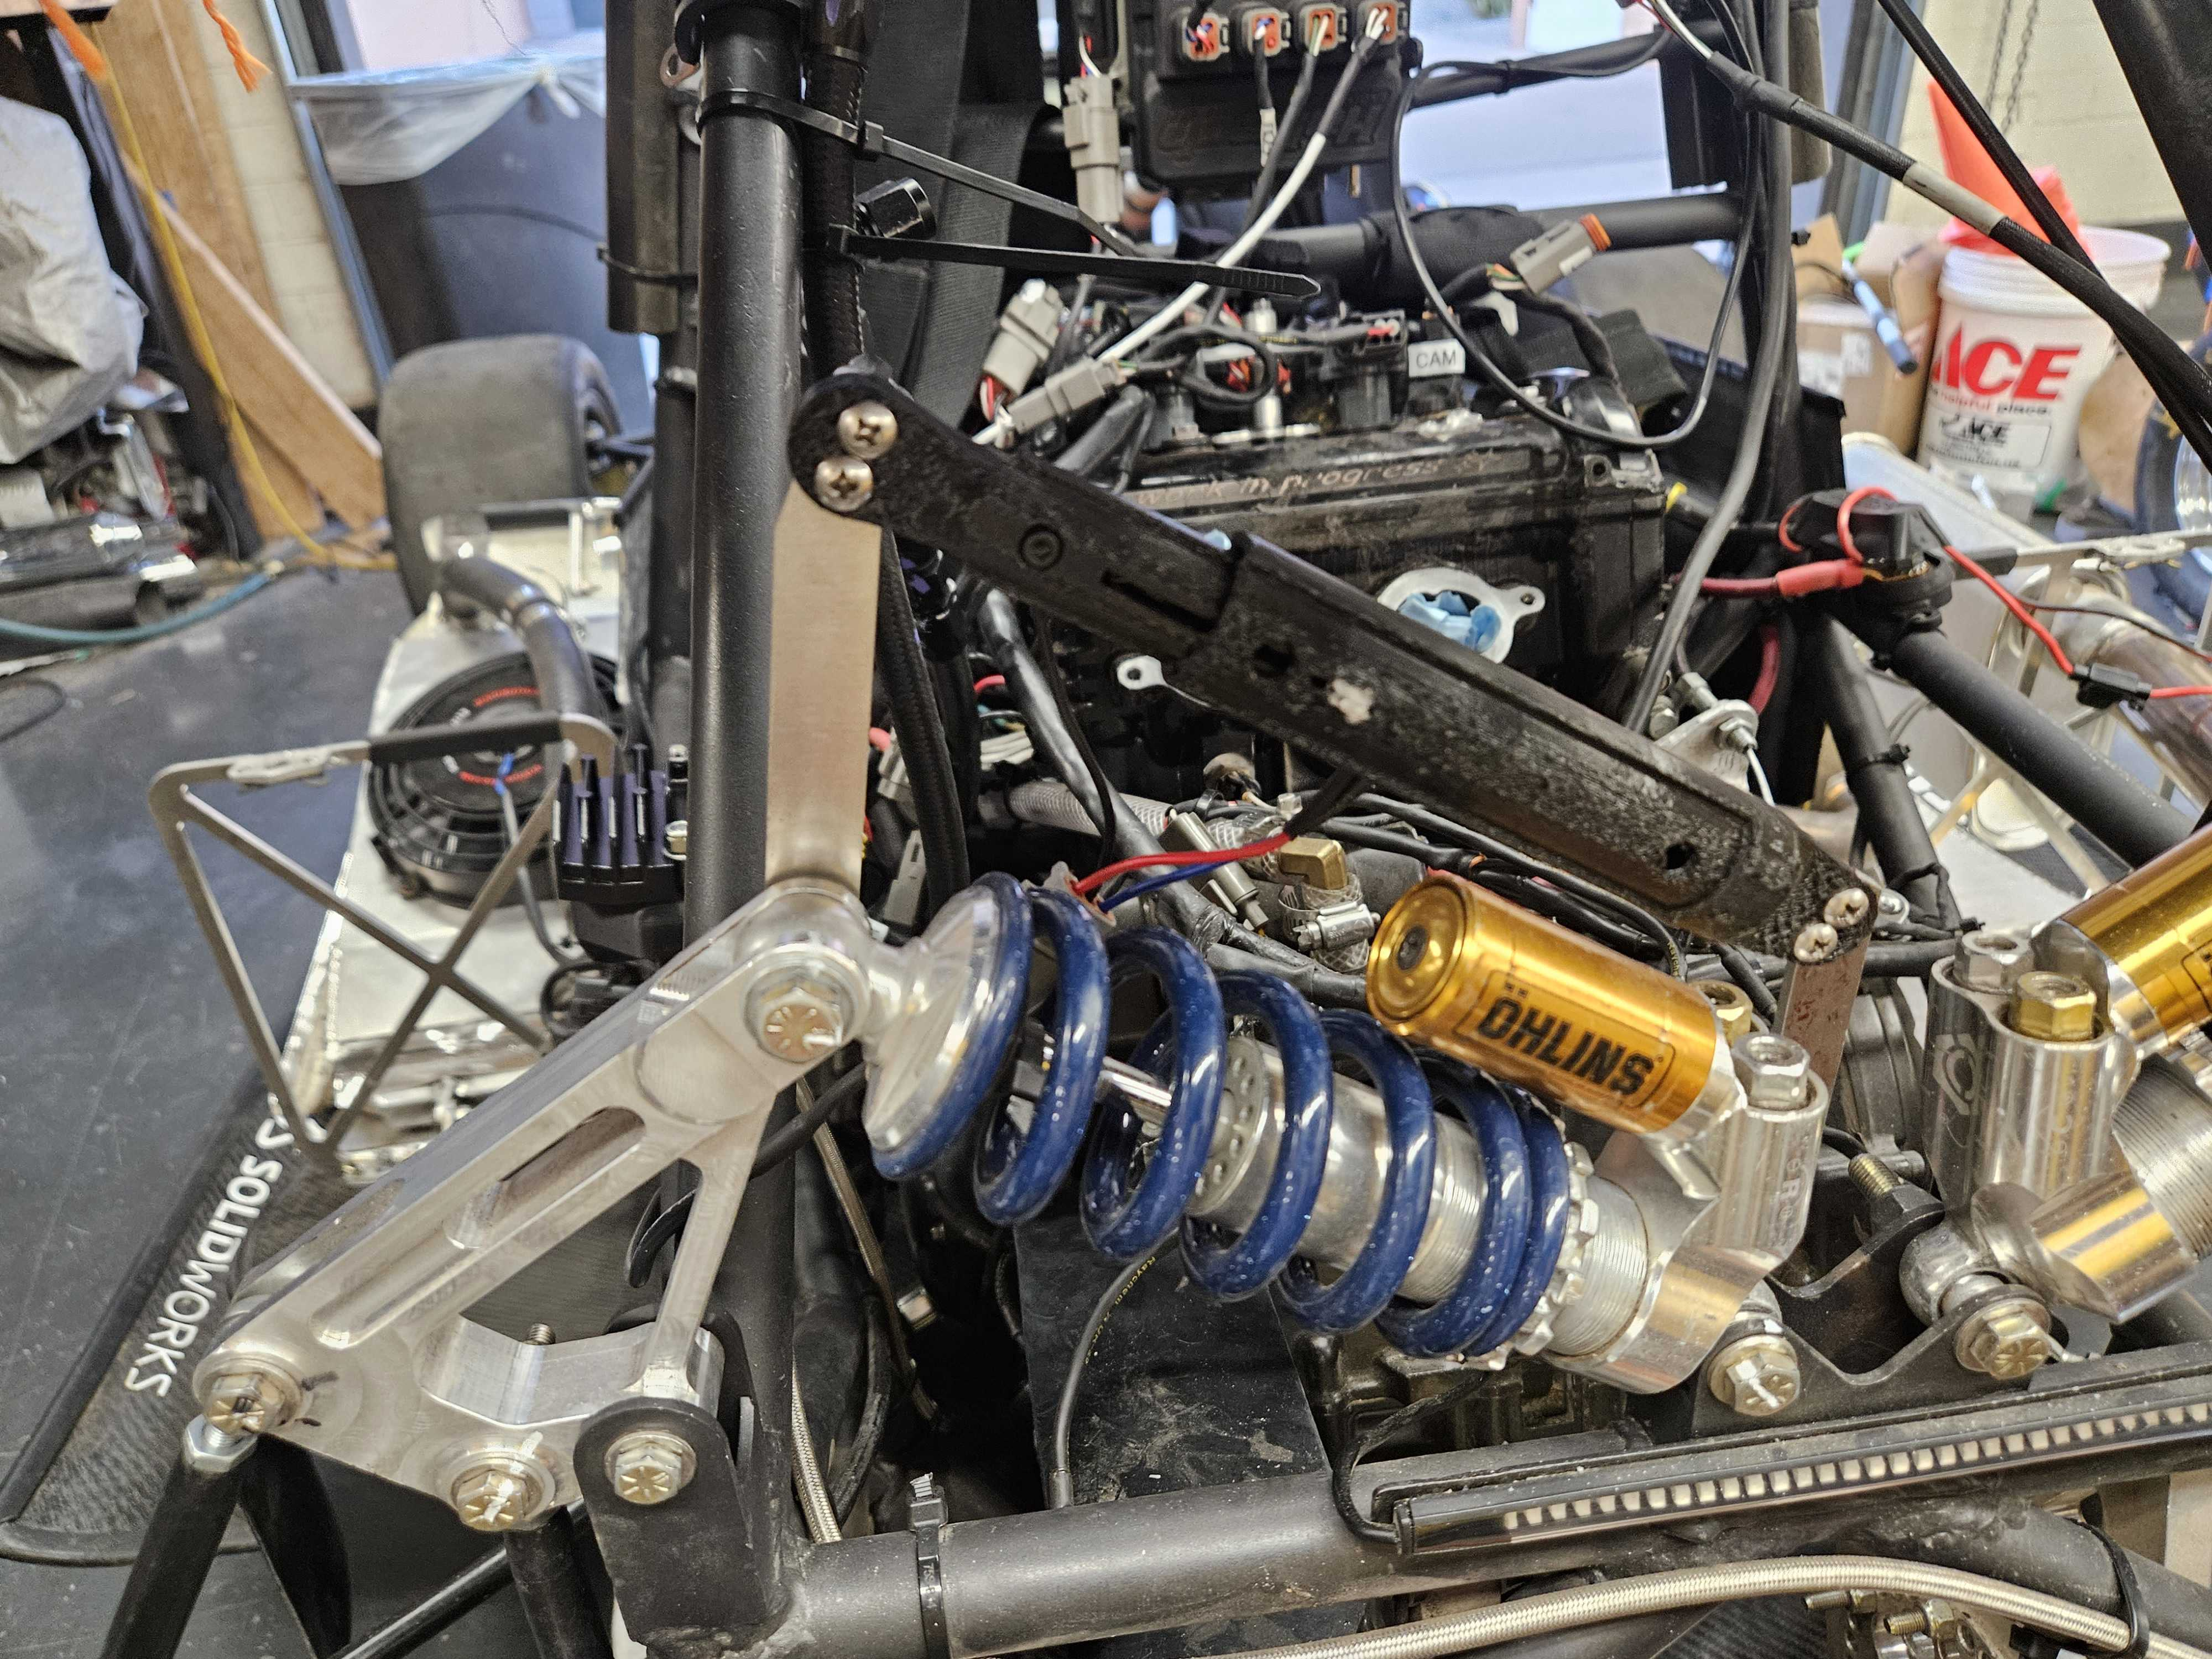
\includegraphics[width=3in]{images/potu.jpg}
    \caption{Damper Potentiometer}
    \label{fig:dp}
\end{figure}
\vspace{1em}

PETG was used instead of ASA to print the 3D-printed parts because PETG is able to bend more before shattering, as this was an issue in prior years.

\section{Steering Angle Sensor Design}
The steering angle sensor consists of the rotary potentiometer, an adapter for the potentiometer knob, and a mount to secure the potentiometer to the steering rack.
The Kaz Technologies Steering Rack includes a keyhole at the bottom of the steering rack around where the steering column is, so the adapter for the potentiometer was designed to fit into this keyhole.
The mount also screws in to 8-32 holes located at the bottom of the steering rack.
\begin{figure}[H]
    \centering
    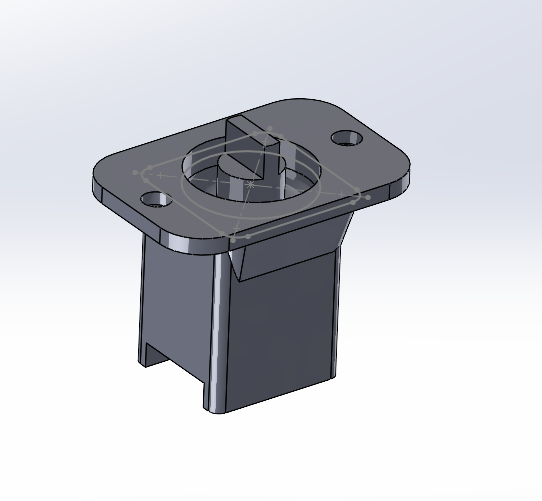
\includegraphics[width=3in]{images/steering.png}
    \caption{Steering Angle Sensor CAD}
    \label{fig:sasc}
\end{figure}

An alternative method of mounting the potentiometer to measure steering angle was a belt and pulley system.
However, given that this method is more complex, we opted to mount the potentiometer at the bottom of the steering rack.

\section{Brake Temperature Sensor Design}
The brake temperature sensor consists of the MLX90614 and a 3D-printed upright mount.
The MLX90614 IR Thermometer is used to measure the temperature of the brake rotors.
The upright mount was printed in PETG, and is designed to clip onto the upright and be secured with an existing fastener.
The MLX90614 is then secured to the mount via super glue.
\begin{figure}[H]
    \centering
    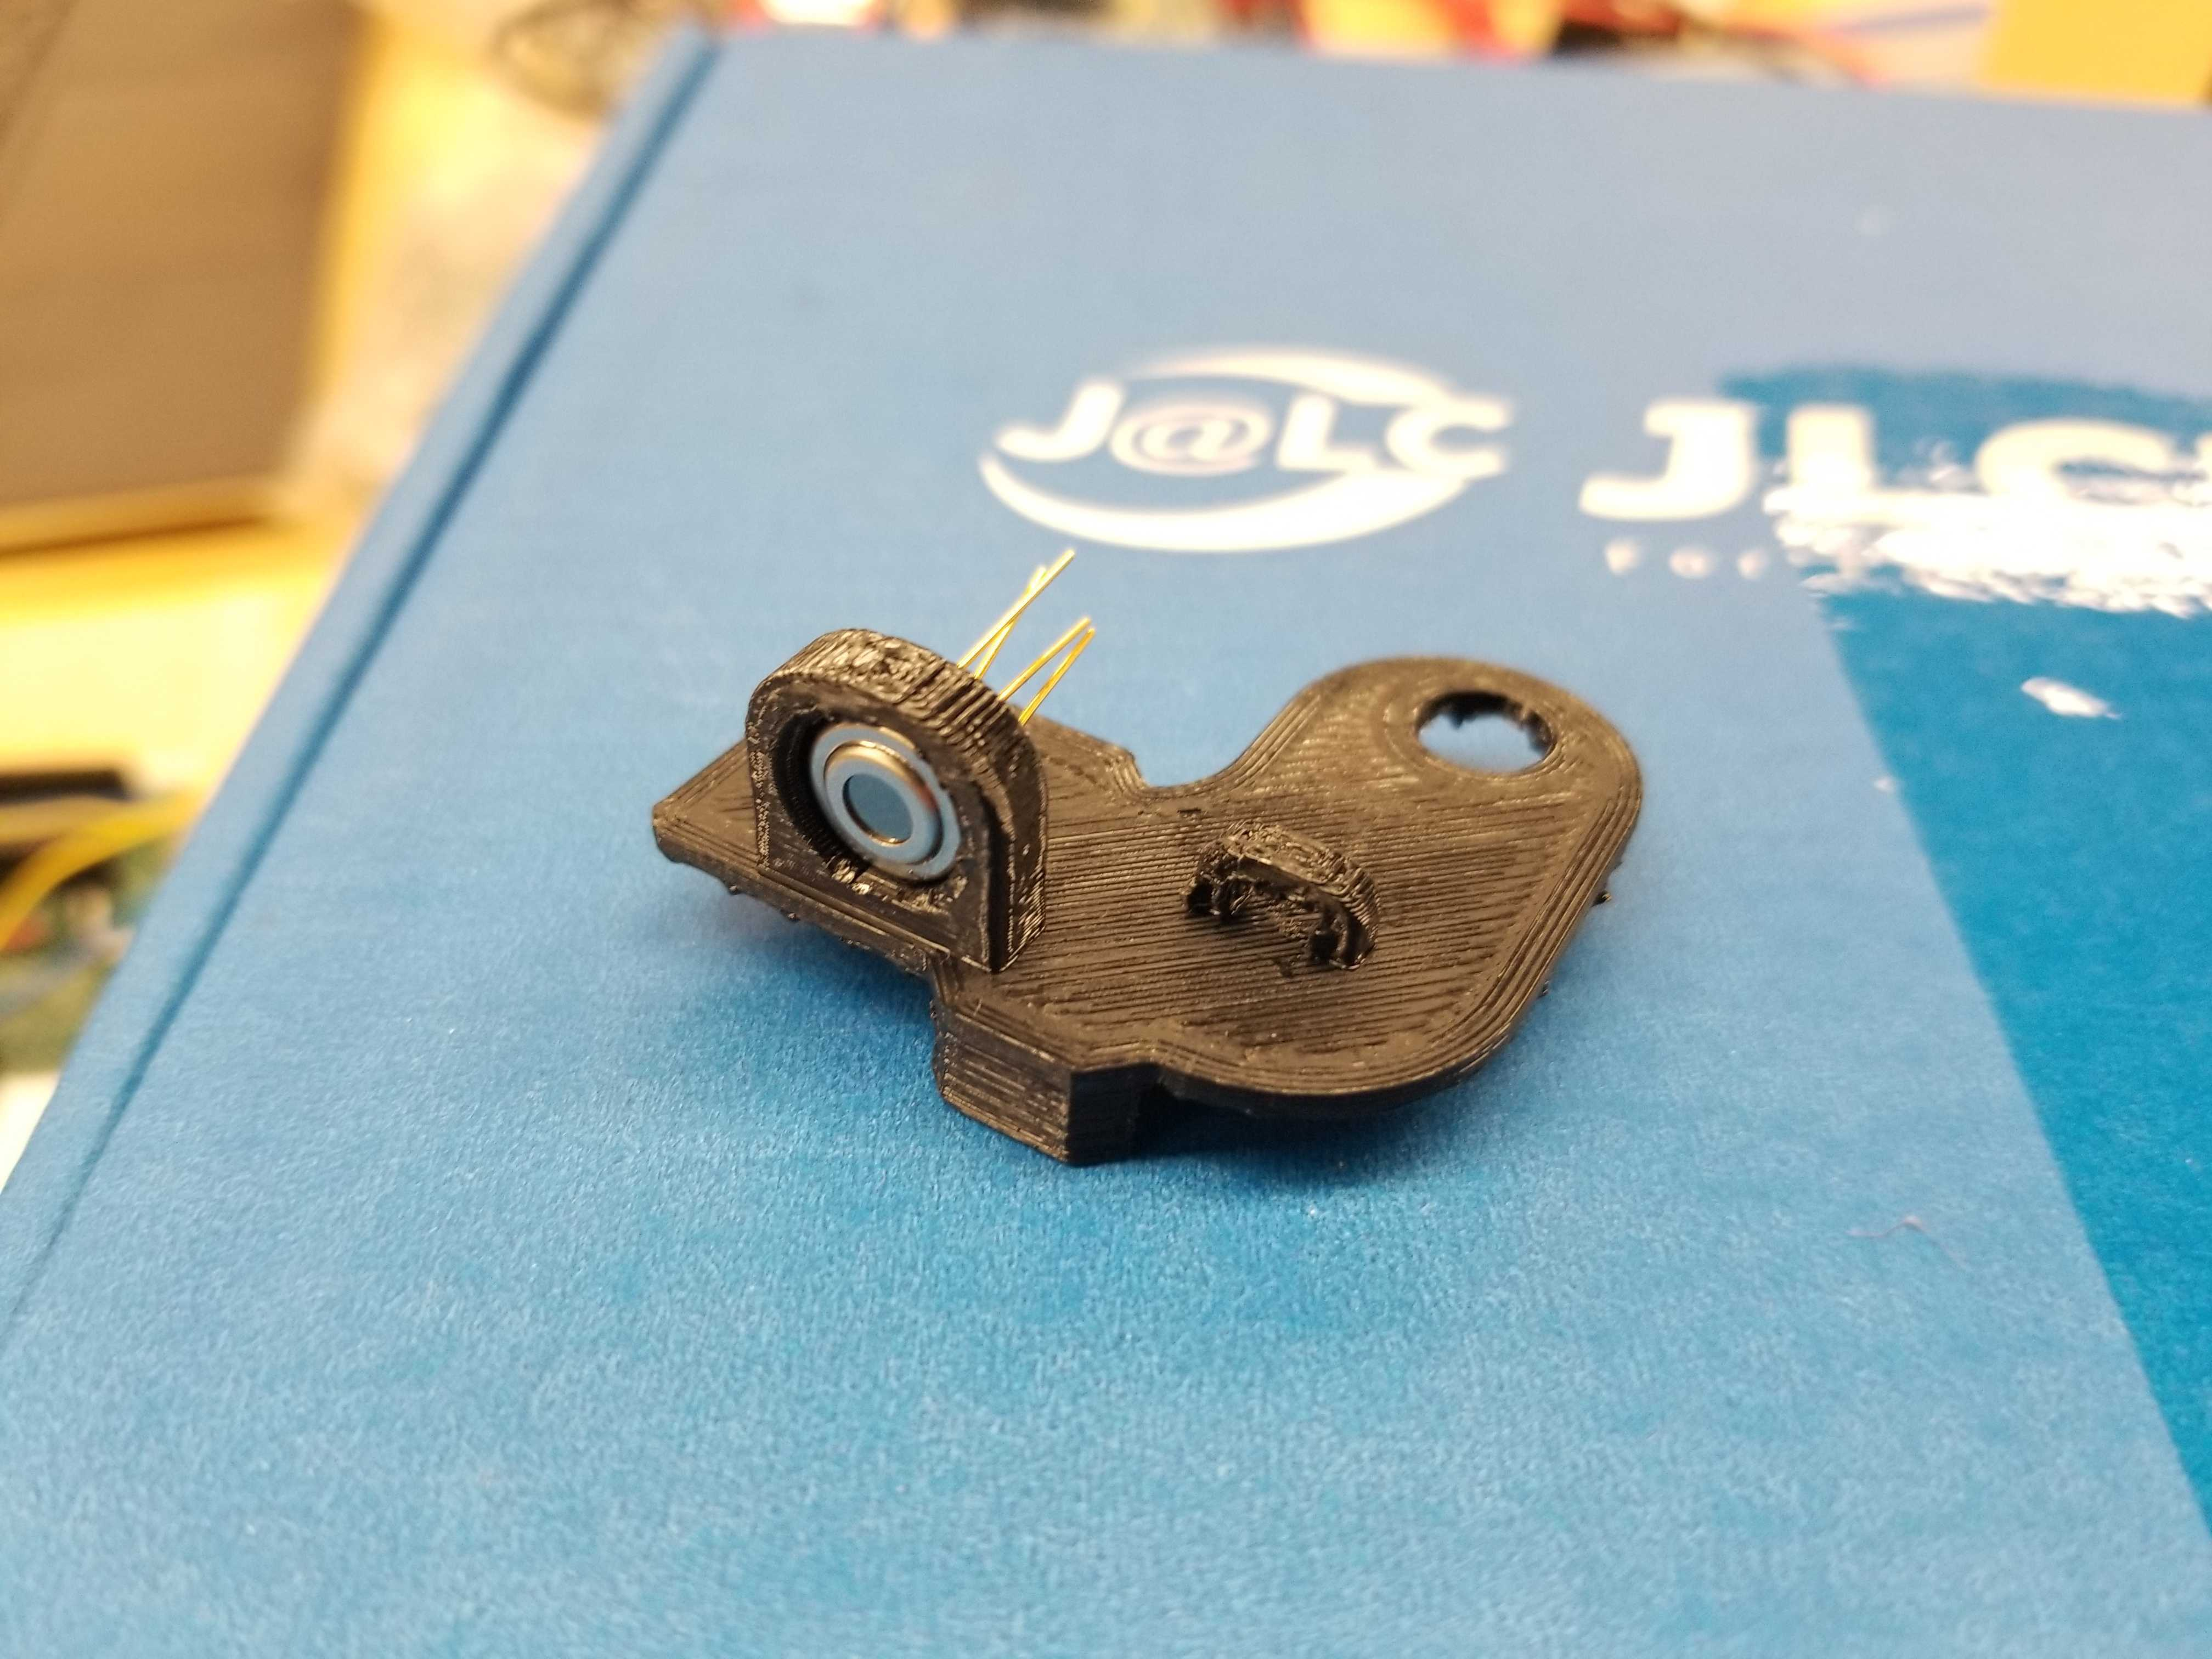
\includegraphics[width=3in]{images/brakes.jpg}
    \caption{Front Brake Temperature Sensor}
    \label{fig:fbts}
\end{figure}
\begin{figure}[H]
    \centering
    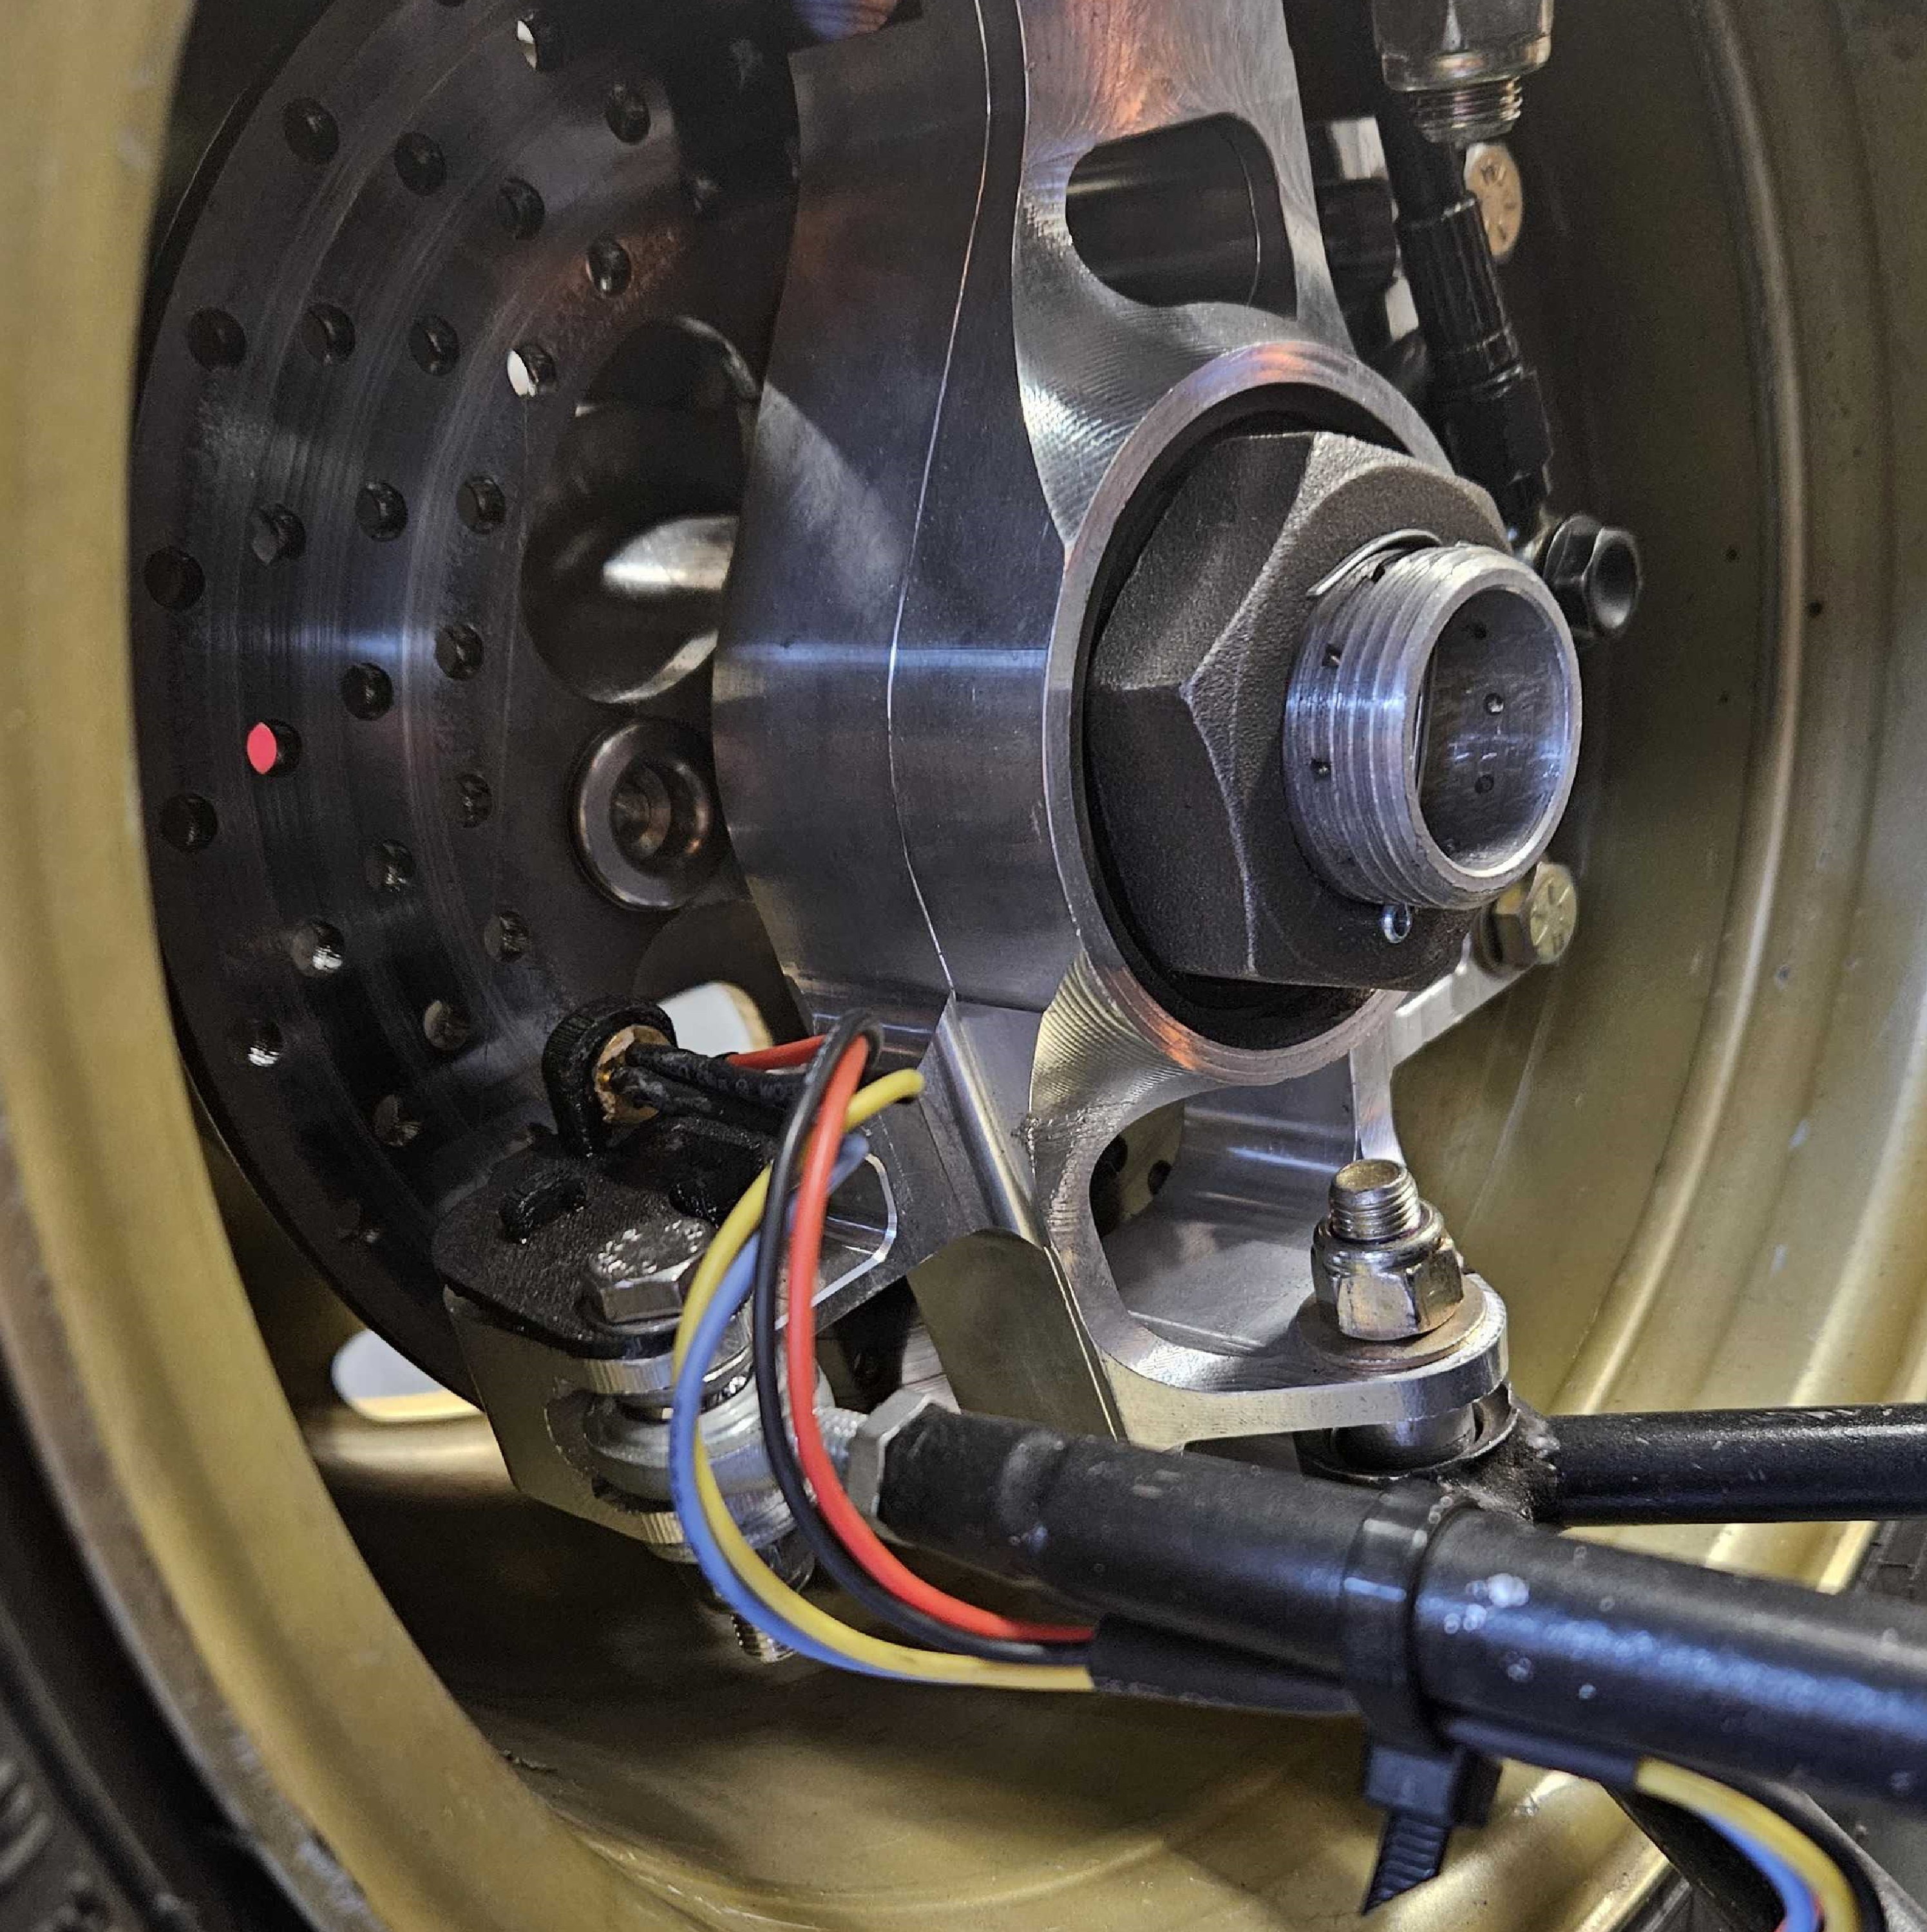
\includegraphics[width=5in]{images/brak.jpg}
    \caption{Installed Brake Temperature Sensor}
    \label{fig:ifbts}
\end{figure}
The MLX90614 library provided by Sparkfun was used to interact with the sensor.
\section{Strain Gauge Amplifier Design}
Although it is possible to hook up the output of a Wheatstone bridge directly to a microcontroller, the voltage difference produced by a bridge is often very minute.
As such, an amplifier board is required to get more precise data out of the bridge.
\vspace{1em}

The design for the strain gauge amplifier board was largely based off of the reference schematic from the HX711's datasheet.
The primary differences are that a Wheatstone bridge completion in a half bridge configuration is present, as well as a jumper to select the data rate.
To ensure the accuracy of the strain gauge, 1\% tolerance resistors were chosen to complete the bridge despite the fact that these are much more expensive.
Since this was the team's first time using the HX711 (or any strain gauge amplifier for that matter), a jumper to select the data rate was included to make the amplifier as flexible as possible.
\begin{figure}[H]
    \centering
    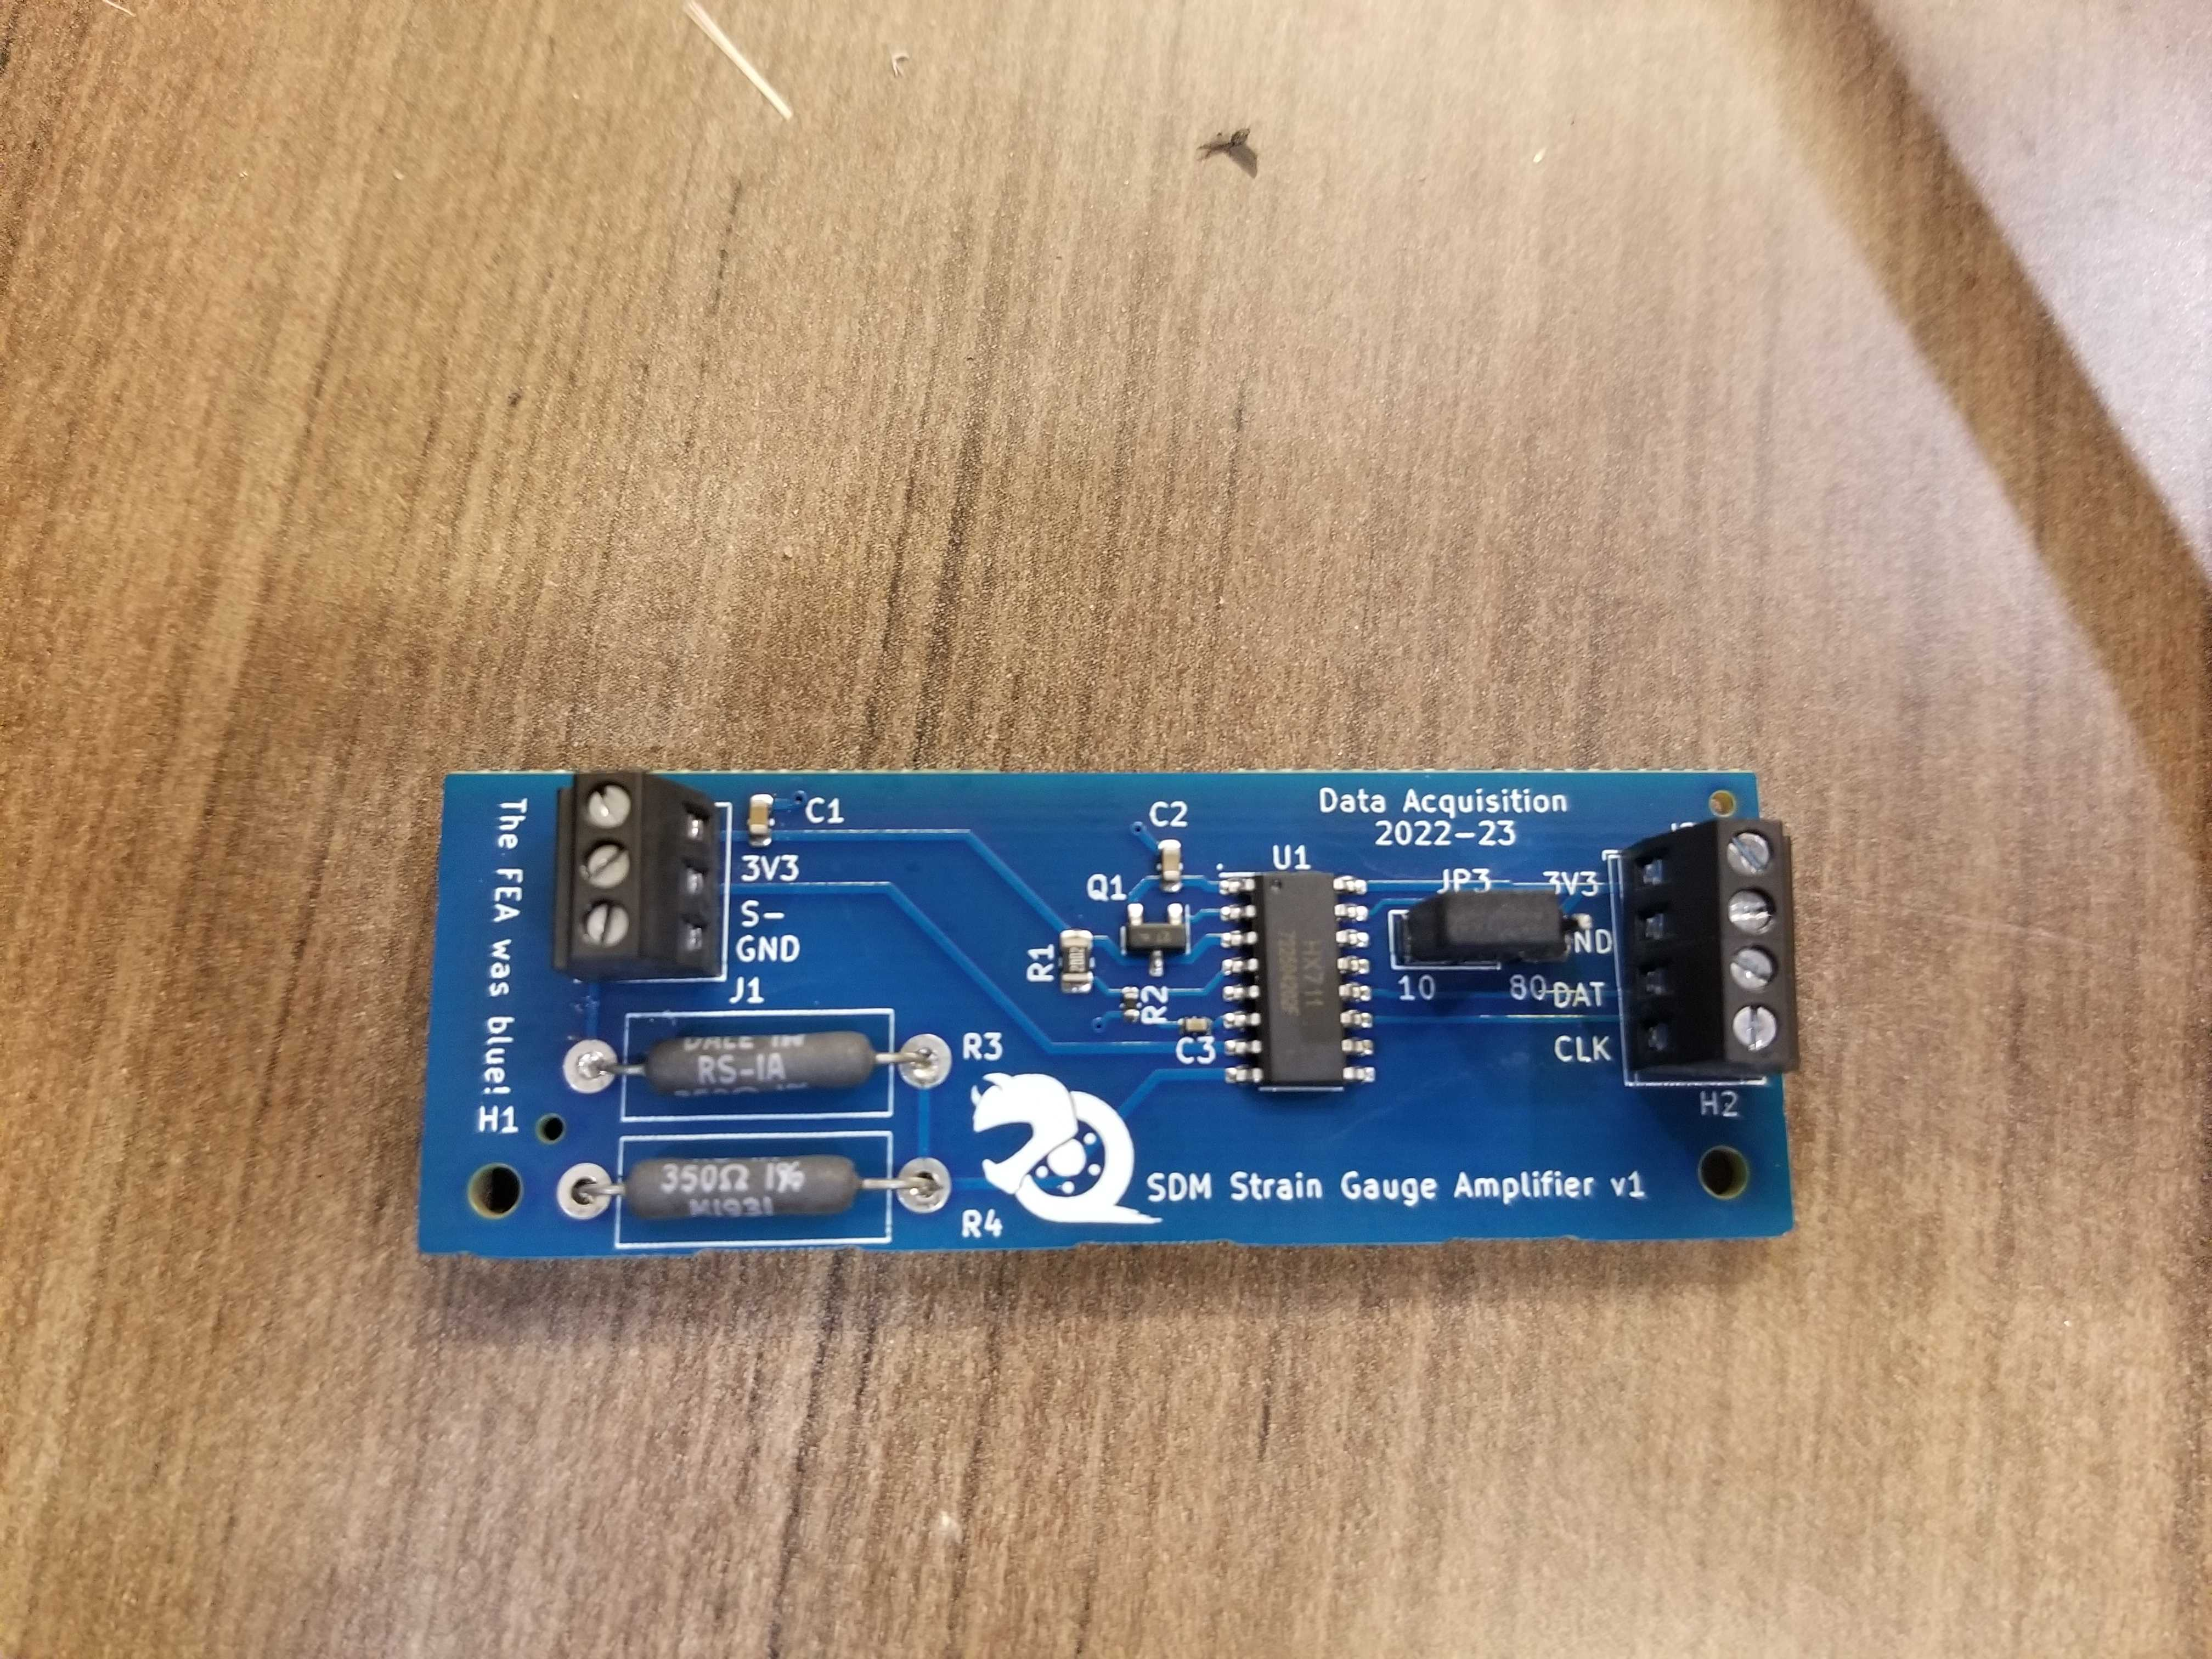
\includegraphics[width=4in]{images/sgamplifier-assembled.jpg}
    \caption{Strain Gauge Amplifier Board}
    \label{fig:sgb}
\end{figure}
A simple enclosure for the board was designed and printed using PETG.
\begin{figure}[H]
    \centering
    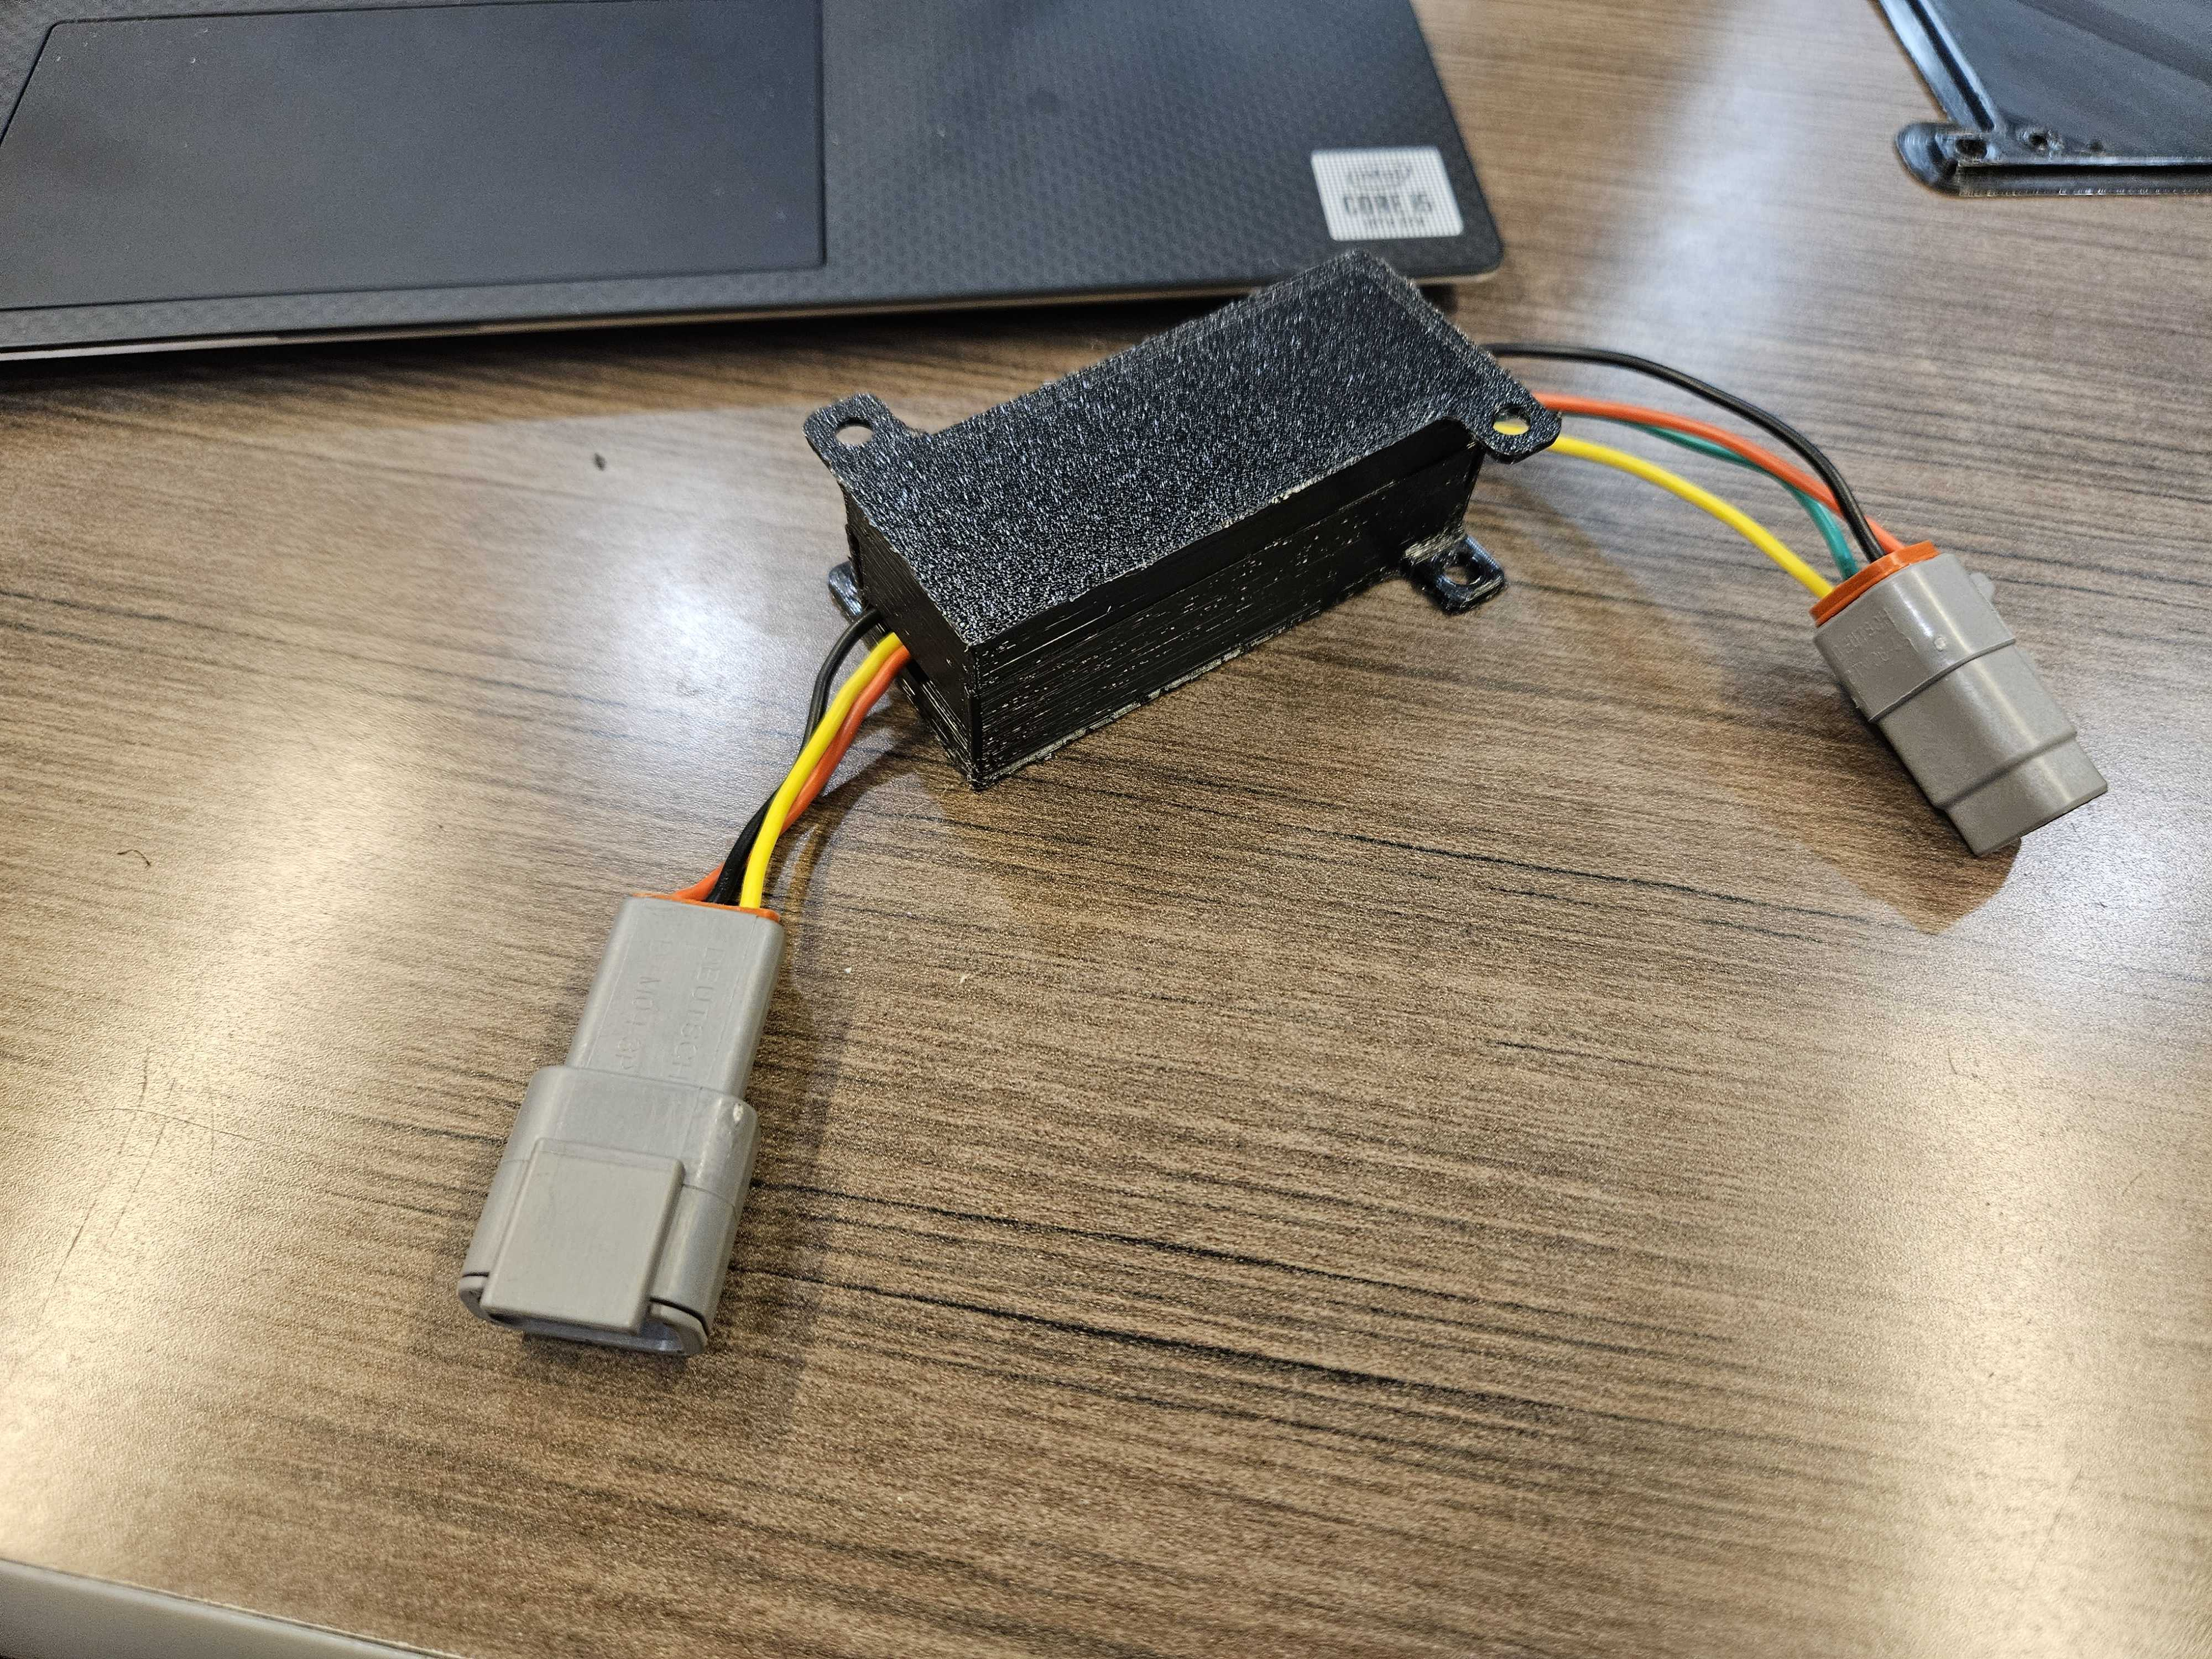
\includegraphics[width=3in]{images/sg-box.jpg}
    \caption{Strain Gauge Amplifier Box}
    \label{fig:sgxb}
\end{figure}

\section{Analysis Software Design}
A collection of software scripts have been developed in order to streamline the data processing pipeline as much as possible.
\begin{figure}[H]
    \centering
    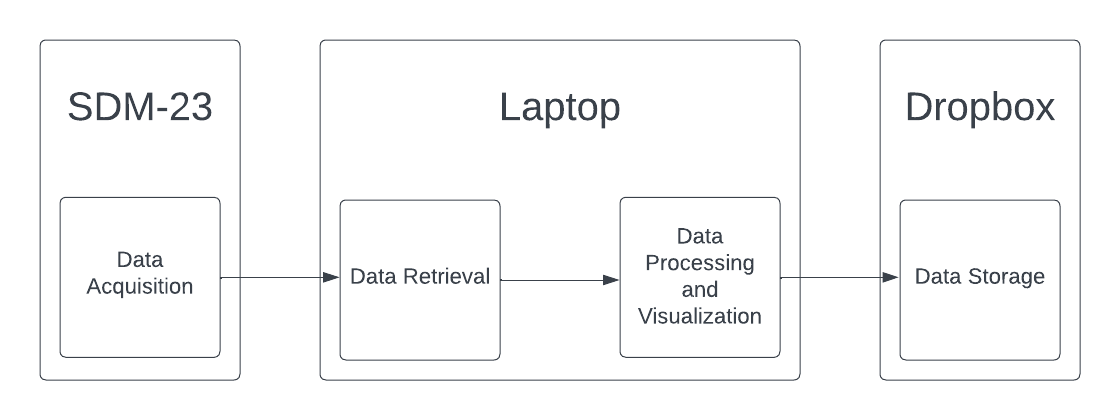
\includegraphics[width=5in]{images/SDM23DataPipeline.png}
    \caption{Data Processing Pipeline}
    \label{fig:dpp}
\end{figure}

\subsection{Data Retrieval}
The primary way of data retrieval is by turning the system off, taking the microSD card and copying the files over to a laptop, then replacing the microSD card in the system.
Although this is a reliable way of retrieving data, given that the main box needs to be disassembled in order to do so does not mean that it is an easy way.
As such, a set of scripts have been developed to retrieve data from the system by plugging the Main box into a laptop via USB:
\begin{itemize}
    \item Discovering Serial Ports
    \item Listing Files
    \item Download All Files
    \item Download Specific File
\end{itemize}
All scripts (with the exception of the discover ports script) follow the general format:
\begin{figure}[H]
    \centering
    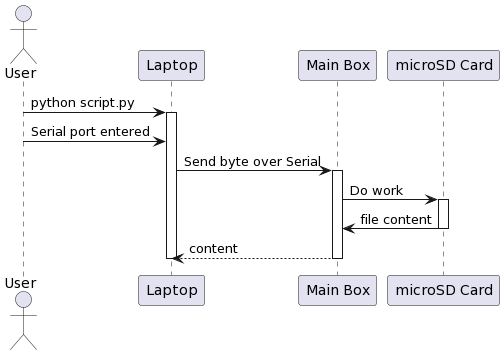
\includegraphics[width=5in]{images/dataretrieval-seq.png}
    \caption{Data Retrieval Script Sequence Diagram}
    \label{fig:drssd}
\end{figure}
The discover ports script is used to determine which serial port to input for the latter three scripts.
The list files script is used to view the files currently on the SD card and can be used in conjunction with the download specific file script, which downloads a specific file onto the laptop.
The last script downloads all files on the SD card onto the laptop.
\begin{figure}[H]
    \centering
    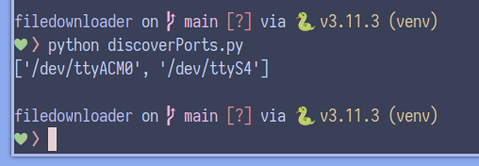
\includegraphics[width=4in]{images/discover.png}
    \caption{Discover Serial ports script output}
    \label{fig:dspsoi}
\end{figure}
\begin{figure}[H]
    \centering
    \includegraphics[width=4in]{images/list.png}
    \caption{List files script output}
    \label{fig:list}
\end{figure}
\begin{figure}[H]
    \centering
    \includegraphics[width=4in]{images/specific.png}
    \caption{Download specific file script output}
    \label{fig:specific}
\end{figure}
\begin{figure}[H]
    \centering
    \includegraphics[width=4in]{images/all.png}
    \caption{Download all files script output}
    \label{fig:all}
\end{figure}
\subsection{Data Processing and Visualization}
Once data has been retrieved from the car, it is moved into a standardized directory structure seen in Figure \ref{fig:dir_struct}:
\begin{figure}[H]
    
    \dirtree{%
    .1 YYMMDD Track Day.
    .2 raw\DTcomment{Folder containing raw data retrieved from DAQ system}.
    .3 morning-session.
    .4 run9-data.csv.
    .4 run10-data.csv.
    .3 arb-test.
    .4 session1.
    .5 run11-data.csv.
    .5 run12-data.csv.
    .4 session2.
    .5 run13-data.csv.
    .5 run14-data.csv.
    .2 interim\DTcomment{Contains processed data with correct units}.
    .3 morning-session.
    .4 run9-data.csv.
    .4 run10-data.csv.
    .3 arb-test.
    .4 session1.
    .5 run11-data.csv.
    .5 run12-data.csv.
    .4 session2.
    .5 run13-data.csv.
    .5 run14-data.csv.
    .2 reports\DTcomment{Contains reports and plots for other subteams}.
    .3 morning-session.
    .4 run9-ggplot.png.
    .3 morning-summary.txt.
    .3 arb-test-session1-summary.txt.
    .3 arb-test-session2-summary.txt.
    .2 generate-ggplot.py.
    .2 generate-summary.py\DTcomment{Creates summary files for raw data}.
    .2 process.py\DTcomment{Processes raw data files to create interim files}.
    .2 requirements.txt\DTcomment{contains Python packages required to run scripts}.
    }
    \caption{Example Directory Structure for Data Processing}
    \label{fig:dir_struct}
\end{figure}
\subsubsection{Summary Generation}
Oftentimes during a testing session, run files are created that are not important to look at, such as when the car is idling or when the car is power cycled.
In order to parse through the run files more efficiently and throw out useless files, a script was created to generate summaries for each run file.
These summaries would include maximum values, ranges and other metrics that can be used to determine if a run file is worth looking closer into.
These metrics include:


\begin{itemize}
    \item maximum absolute lateral acceleration value
    \item minimum and maximum acceleration value
    \item brake pressure range
    \item maximum brake rotor temperature
    \item damper travel range
    \item maximum GPS ground speed value
    \item GPS fix acquired time
    \item Run file duration
\end{itemize}
\begin{figure}[H]
    \centering
    \includegraphics[width=4in]{images/summary.jpg}
    \caption{Example Run File Summary}
    \label{fig:sum}
\end{figure}
At the end of each summary, various lists of run numbers are created to give an overview of what run files fulfill a given metric.
\begin{figure}[H]
    \centering
    \includegraphics[width=4in]{images/sessionsumarry.jpg}
    \caption{Example Session Summary}
    \label{fig:sessionsumum}
\end{figure}
The summary files also give insight into any issues the DAQ system may have had while collecting data.
For instance if a box had power issues or a sensor was malfunctioning, the summary file would generally be able to catch that.
\subsubsection{Interim File Generation}
After summary files have been created, a script is used to generate interim run files.
These interim files have corrected units (e.g., for a steering angle sensor, the channel would have degrees instead of the raw ADC value) and drop any unused columns.
As such these are better suited to use for creating plots and diagrams as opposed to the raw files produced by the DAQ system.
\vspace{1em}

The \texttt{pandas} library is used to process and generate interim files.
\subsubsection{Plot and Diagram Generation}
A function was created for each kind of plot or diagram that was to be made, which would take a path, run number, and a force boolean as input.
If the force boolean evaluated to false, then simple criteria would be used to determine if a plot for the given run number and path would be generated, which was useful for automatically generating plots.
For example if the plot was brake rotor temperature vs time, then a check for the rotor temperature range would determine if a plot would be generated or not.
\vspace{1em}

\texttt{matplotlib} and \texttt{pandas} are used for plot and diagram generation.

\subsubsection{Lap Generation}
It is important to create a distinction between laps and laptimes during tests/races. Data visualization is a process which encapsulates this need and enables the ability to better our results through data. Using GPS data consisting of latitude/longitude alongside timestamps, we can acquire this data.
The lap generation program uses python notebooks utilizing pandas and matplotlib and encapsulates the data from csv in a dataframe. Our determination of a new lap utilizes a radius from the beginning point where this acts as a threshold to determine whenever the car passes this point. To determine whether the current point is within the threshold, the distance between points needs to be calculated. The calculation determines the distance between the first node detected and the current node within the dataframe. The equation is as follows:
\begin{gather}
    D_{a,b} = \sqrt{(\Delta latitude)^2 + (\Delta longitude)^2} 
\end{gather}

Once a distance between two points is acquired, we compare this to our selected radius threshold to determine whether our lap counter should be incremented. Iterating through our dataframe with the process described above will yield the ability to count the number of laps quantitatively and as well enable us to visualize the laps on a map. This visualization can be seen in a multitude of ways. To visualize how our laps are counted, one can plot a distance vs time graph where distance is the displacement of the car from a arbitrarily chosen location. A sample graph is provided: 

\begin{figure}[H]
    \centering
    \includegraphics[width=5in]{images/distancevtime.png}
    \caption{Distance vs Time Graph}
    \label{fig:dtg}
\end{figure}

\vspace{1em}

Additionally, there is a possible roadmap for where this track map can go. Firstly, we can overlay the laps on to a map provided by openstreetmap and see where our data was gathered geographically. While not impressive currently, this provides the framework for the team to expand upon this idea to sort and parse this data to make it more viable for the team. Examples of this should include showing singular laps at a time, color-coding based on lateral acceleration, and viewing racing lines. A picture of this is provided:

\begin{figure}[H]
    \centering
    \includegraphics[width=5in]{images/map.png}
    \caption{OpenStreetView Map}
    \label{fig:osvm}
\end{figure}

\subsection{Data Storage}
All raw and interim files, as well as any generated reports and notes, are stored on the team's Dropbox and can be viewed and downloaded by anyone on the team with access to it.
For SDM-23 Track Day data, a directory spreadsheet was created to help the team find data they are looking for.
This directory includes:
\begin{itemize}
    \item Date of track day
    \item A Data Quality Rating
    \item Sensor availability
    \item Notes
    \item Link to data folder in Dropbox
\end{itemize}
The Data Quality Rating is a rating from 1 (unusable) to 10 (good) based on how reliable the DAQ system was for the given track day that was qualitatively determined by the DAQ subteam.
The sensor availability chart gives a simple rating for each sensor.
If the cell is green, then the data produced by the sensor was consistent and likely usable.
If the cell is yellow, then the data produced was of mixed quality, or is partially missing.
If the cell is red then no data was collected from that sensor for the given track day.

These two metrics and the testing notes give an overview for team members to easily determine and find where data for a given track day is.
\begin{figure}[H]
    \centering
    \includegraphics[width=7in]{images/tddr.jpg}
    \caption{SDM-23 Track Day Data Directory}
    \label{fig:tddr}
\end{figure}


\chapter{Results}
This chapter will go over the results of the manufacturing of the DAQ system as well as its performance and reliability during SDM-23's track days.

\section{System Manufacturing}
Although the DAQ system was designed with a Rear I/O box in mind, this box was never designed nor manufactured due to time constraints, which severely affected our ability to collect data at the rear of the car.
The design deadline set by the team was also not respected.
\subsection{Wiring Manufacturing}
The original design for the DAQ system utilised Binder 719 connectors, which were selected because they came in panel-mount versions and because they are prevalent in AiM systems.
These were assembled by soldering wires to the solder cups on the connectors.
Although they were small and lightweight, they were very difficult and time-consuming to solder and assemble, and were prone to creating shorts in the wires due to soldering errors.
\vspace{1em}

As such, the decision was made partway through the manufacturing phase to switch over to DTM connectors for all connections, which required crimping terminals onto wires instead of soldering them.
Although DTM connectors are much larger (a size comparison with a DT connector is shown in Figure \ref{fig:binderbad}), their crimp termination meant that assembling these connectors are much easier and less prone to human error.
It should be noted that although this delayed the completion of the DAQ system as the PCB enclosures needed to be redesigned for the larger connectors and for the DTM connectors to arrive, this greatly increased the reliability of the DAQ system and made it faster and easier to manufacture the rest of the system.
\begin{figure}[H]
    \centering
    \includegraphics[width=4in]{images/binder.jpg}
    \caption{Size comparison between a Binder 719 and a DT connector}
    \label{fig:binderbad}
\end{figure}

\subsection{Sensor Calibration}
\subsubsection{Brake Pressure Sensor}
The transfer function for the brake pressure sensor has been given by Honeywell in the product datasheet.
However since a voltage divider was used to step down the output from the brake pressure sensor into a suitable range for the Teensy, this must be accounted for before using the provided transfer function.
First, the raw ADC value is converted to volts:
\begin{gather}
    V_{3.3}(a) = a\cdot \frac{3.3}{1023}
\end{gather}
This is converted into a 5V range by using the inverse of the voltage divider (Using 6.8k$\Omega$ for $R_1$ and 10k$\Omega$ for $R_2$):
\begin{gather}
    V_5(v) = 1.68\cdot v
\end{gather}
Once a voltage value in the range $[0,5]$ has been obtained we can then use the transfer function in Equation \ref{eq:bps} to get a brake pressure value.

\subsubsection{Brake Rotor Temperature Sensor}
Initially, the setup code for the MLX90614 would set the emissivity value of the sensor on every startup.
However, this would cause the sensor to sometimes read negative values during the duration of a run, which is obviously not correct, an example seen in Figure \ref{fig:hehehehehe}.
\begin{figure}[H]
    \centering
    \includegraphics[width=3.5in]{images/negativetemp.png}
    \caption{MLX90614 reading negative temperatures}
    \label{fig:hehehehehe}
\end{figure}
Upon further investigation, an issue on the MLX90614 library's GitHub page found that power cycling the sensor after changing the emissivity would solve the issue.
It was also determined that the emissivity value used by the sensor is saved internally in the sensor, so there is no need to set the emissivity every time the DAQ system turned on.
\vspace{1em}

After removing the emissivity line, the MLX90614 no longer read negative values, with the only issue remaining is that the sensor's object temperature reading would spike to a five figure number.
As of the time of writing, this has not been solved yet.
A quick fix that can be applied during data processing is to throw out the spike.
\begin{figure}[H]
    \centering
    \includegraphics[width=3.5in]{images/hot.png}
    \caption{Temperature spike in the MLX90614 output}
    \label{fig:hot}
\end{figure}
\subsubsection{Damper Potentiometer}
Since the same potentiometer model was used from SDM-22, the transfer function created for that year was carried over, with the only addition being that the units changed from inches to millimeters.
\begin{gather}\label{eq:dptf}
    P(a) =  0.053440584\times a
\end{gather}
Equation \ref{eq:dptf} shows the transfer function $P(a)$ that outputs the potentiometer's current position in millimeters given the 10-bit ADC value $a$.
During the data processing stage, damper displacement and velocity would be calculated using this value.
\subsubsection{Gyroscope}
At the time of writing, the gyroscope settings have not been sufficiently tuned to produce consistent angular position data due to lack of time.
The gyroscope debugger requires more work in order to be useful, as there was a significant delay in moving the IMU unit and the data showing up on the debugger.
\vspace{1em}

Another consideration that should be made is how the IMU is mounted in the car, as the IMU had a lot of rotational slack.
\subsubsection{Steering Angle Sensor}
From testing the rotary potentiometer, we found that it had a linear slope and did not have a hard stop.
Once it was installed onto the steering rack, we found the following values for the steering wheel's center, right, and left positions:
\begin{table}[H]
    \centering
    \begin{tabular}{|c|c|}
        \hline
         Steering Wheel Angle & ADC output of potentiometer \\
        \hline
         center & 102 \\
         90 degrees right & 337 \\
         90 degrees left & 902 \\
        \hline
    \end{tabular}
    \caption{Calibration values for the Steering Angle Sensor}
    \label{tab:sas}
\end{table}
As seen in Table \ref{tab:sas}, the potentiometer ``overflows'' when turning the wheel left.
As such the transfer function for the steering angle sensor would need to be piecewise:
\begin{gather}
    A(a) = \begin{cases} 
      0.392\cdot a - 42.176 & a \leq 500 \\
      0.392\cdot (a - 1024) - 42.176 & a > 500 \\
   \end{cases}
\end{gather}
$A(a)$ returns a value in degrees where $a$ is the ADC value of the rotary potentiometer.
A positive value would indicate turning right, while a negative value would indicate turning left.
Zero indicates the steering wheel is centered.

\subsubsection{Strain Gauges}
At the time of writing, the strain gauge output have not been used or validated.
There were also issues with the strain gauges, likely stemming from manufacturing errors in either the bonding process or the strain gauge amplifier assembly.
The output from the front left strain gauge on the push rod was wildly inconsistent.
In other instances, the strain gauge output would stick at $50\%V_{in}$. 

\section{System Performance}
\subsection{Electrical Performance}
Throughout SDM-23 testing, electrical reliability was the DAQ system's greatest weakness.
Poor and/or inconsistent solder joints in the PCBs would result in either loss of power in some boxes or loss of data transmission, both cases severely affecting data collection during track days.
Loss of power and/or data transmission was detected by inspection of the summary files, finding plateaus in the data (Figure \ref{fig:los} demonstrates this), or by visual inspection of the box (if a Teensy LED for a box was not lit, this would usually indicate power loss).
\begin{figure}[H]
    \centering
    \includegraphics[width=4.5in]{images/data-loss.png}
    \caption{Instance of loss of power/data transmission by the Front IO box}
    \label{fig:los}
\end{figure}
In general, these were able to be diagnosed via continuity and voltage checks with a multimeter.
\vspace{1em}

Early on in SDM-23 testing, CAN data would occasionally drop from the driver dashboard.
This was easily fixed by removing the terminating resistor on the ECU CAN transceiver in the Main box.

\subsection{Mechanical Performance}
The mechanical aspect of the DAQ system worked as intended, as all the sensor mounts were able to hold up during track days.
One area for improvement would be to design more robust PCB enclosures, as it was difficult to plug or unplug connectors because if too much force was used the enclosure could shatter, so to avoid that occurring the receptacle would be held while plugging/unplugging the connector.

\subsection{Software Performance}
In most cases, the DAQ system's software worked as intended.
However, there were instances where the software failed due to relatively simple errors.
\vspace{1em}

One software fault was selecting the wrong Serial port to use for communication with the GPS module, which caused us to not collect any GPS data during one of the track days.
Another software fault was not logging steering angle data to the SD card.
Both of these faults could've been easily caught in a software review.
\vspace{1em}

A third software fault was not logging GPS position data and timestamps to a sufficient enough precision.
In the first case, this caused the GPS position data to be inaccurate and effectively useless.
The second case would cause issues when doing any calculations with a difference between consecutive timestamps, as there would be occasional duplicate timestamps.
Both cases were solved by logging these channels with additional precision: GPS position data would be logged to four decimal places while timestamps would be logged to three decimal places.


\chapter{Conclusion and Future Work}
During the course of the 2022-23 school year the DAQ team was able to create the foundations for a usable data acquisition system.
Despite being perpetually behind in both the design and manufacturing phases, we were able to provide value to the rest of the team by validating aspects of the brakes and suspension designs.
When the system was not plagued with electrical issues, most of the sensors installed in SDM-23 were relatively free of noise when compared to prior years.

\section{Electrical Recommendations}
Given that much of the failures of the DAQ system this year was attributed to soldering mistakes, more care should be taken when assembling the PCBs.
Although using breakout boards were useful for prototyping, given that the solder joints for these boards were a common failure point, it is recommended to layout the circuitry directly onto the PCB for future designs.
\vspace{1em}

Another recommendation for future PCB design is to look into wire-board connectors, such as JST or Molex connectors, as an alternative to screw terminal blocks.
Although the screw terminals are easy to work with, given that the DAQ system will experience vibrations (racecar duh) screw terminals are not very viable as they could become unscrewed during vehicle operation.
Another alternative is to use connectors with PCB headers, which would completely eliminate the failure point between the enclosure connector and the PCB connector.

\section{Mechanical Recommendations}
As described in the previous chapter, future PCB enclosures could be designed to be more robust so that extra care when plugging/unplugging connectors does not need to be made.
Additionally, the PCB enclosures were not designed to be waterproof and were generally deemed to be ``waterproof enough."
Although this is not typically an issue for Arizona, since the competition will almost always be out of state it is recommended to design future enclosures to be waterproof.
\vspace{1em}

One last recommendation for the mechanical aspect is to work more closely with the rest of the team to design sensor mounts and for processing data.
For instance dedicated mounting holes on the upright for the brake temperature sensor would mean that we would not have to use an existing hole or mount using velcro.
It is also important to work with the rest of the team to better understand the mechanical systems that we are measuring and making sure they are able to make use of the data, especially when it comes to making use of the strain gauge data.

\section{Software Recommendations}
Towards the end of SDM-23's testing and validation phase, the DAQ team would go through line by line each of the code that was uploaded to the Teensy boards before a testing day to ensure there were no software faults.
This could be extended by conducting software development on a \texttt{develop} branch in the Git repository, and merge to the \texttt{main} branch after a pull request review for a track day.
In doing so, the DAQ team would have a stable version of the software for use during track days and be able to easily identify changes between versions.
\vspace{1em}

Much work can be done to improve the data retrieval, processing, and visualization portions of the data pipeline.
Work is currently being conducted to make a GUI for the data retrieval scripts, which will allow non-software-minded people to easily retrieve data.
Another project that would improve the processing and visualization steps is a data explorer GUI, which would allow a user to ``explore" a file in greater detail than viewing a summary of the file.
Such a project should also incorporate utilities for generating laps and lap times, i.e. selecting a finish line location on the map of the GPS data, as well as for generating other common plots and data visualizations.
An alternative to this project could also be finding some way to integrate the DAQ system to produce files for professional software such as Race Studio 3, which would save a lot of development time and also teach team members how to use software used in the motorsport industry.


\appendix

\chapter{DAQ Interface Control Document}
\section{Main Box}
\begin{figure}[H]
    \centering
    \includegraphics[width=3in]{images/pcbmain.png}
    \caption{Main box PCB}
    \label{fig:pcbmain}
\end{figure}
\begin{itemize}
    \item Connects to: Haltech ECU, IMU box, GPS Antenna, damper potentiometer
    \item Overall functions: Logging CAN data
\end{itemize}
\subsubsection{Physical I/O}
\begin{figure}[H]
    \centering
    \includegraphics[width=7in]{images/piomain.png}
\end{figure}
Other physical I/O include an SMA connector for a GPS antenna and a micro USB for data retrieval and Teensy programming.
\subsubsection{Digital Interfaces}
N/A

\section{IMU Box}
\begin{figure}[H]
    \centering
    \includegraphics[width=3in]{images/pcbimu.png}
    \caption{IMU box PCB}
    \label{fig:pcbimu}
\end{figure}
\begin{itemize}
    \item Connects to: Main box, Front I/O box
    \item Overall functions: Reading IMU data and transmitting it over CAN
\end{itemize}
\subsubsection{Physical I/O}
\begin{figure}[H]
    \centering
    \includegraphics[width=7in]{images/pioimu.png}
\end{figure}
\subsubsection{Digital Interfaces}
\begin{figure}[H]
    \centering
    \includegraphics[width=7in]{images/dioimu.png}
\end{figure}

\section{Front I/O Box}
\begin{figure}[H]
    \centering
    \includegraphics[width=3in]{images/pcbio.png}
    \caption{IO box PCB}
    \label{fig:pcbio}
\end{figure}
\begin{itemize}
    \item Connects to: IMU box, steering angle sensor, brake pressure sensors, strain gauge amplifier, brake rotor temperature sensor
    \item Overall functions: Reading sensor data and transmitting over CAN
\end{itemize}
\subsubsection{Physical I/O}
\begin{figure}[H]
    \centering
    \includegraphics[width=5.5in]{images/pioio.png}
\end{figure}
\subsubsection{Digital Interfaces}
\begin{figure}[H]
    \centering
    \includegraphics[width=7in]{images/dioio.png}
\end{figure}

\chapter{Mass Breakdown}
\begin{center}
\begin{tabular}{|c|c|}
    \hline
    Part & Mass (g) \\
    \hline
    Main Box & 262\\
    IMU Box & 116\\
    Front I/O Box & 414\\
    Rear Shock Pot & 50\\
    Brake Temperature Sensor & 8\\
    Strain Gauge Amplifiers & 88\\
    Steering Angle Sensor & 40\\
    Brake Pressure Sensors & 66 \\
    \hline
    \hline
    Total & 1044 \\
    \hline
\end{tabular}
\end{center}

\glsaddall % add all acronym entries
\newacronym{cad}{CAD}{Computer-Aided Design}
\newacronym{can}{CAN}{Controller Area Network}
\newacronym{daq}{DAQ}{Data Acquisition}
\newacronym{gpio}{GPIO}{General-Purpose Input/Output}
\newacronym{imu}{IMU}{Inertial Measurement Unit}
\newacronym{i2c}{I2C, I$^2$C}{Inter-Integrated Circuit}
\newacronym{pcb}{PCB}{Printed Circuit Board}
\newacronym{sdm}{SDM}{Sun Devil Motorsports}
\newacronym{sd}{SD}{Secure Digital}
\newacronym{ecu}{ECU}{Electronic Control Unit}
\newacronym{gps}{GPS}{Global Positioning System}
\newacronym{smt}{SMT}{Surface-Mount Technology}
\newacronym{asu}{ASU}{Arizona State University}
\newacronym{gui}{GUI}{Graphical User Interface}
\newacronym{esd}{ESD}{Electrostatic Discharge}
\newacronym{io}{I/O, IO}{Input/Output}
\newacronym{petg}{PETG}{Polyethylene Terephthalate Glycol}
\newacronym{pla}{PLA}{Polylactic Acid}
\newacronym{usb}{USB}{Universal Serial Bus}
\newacronym{ice}{ICE}{Internal Combustion Engine}
\newacronym{sae}{SAE}{Society of Automotive Engineers}
\newacronym{adc}{ADC}{Analog-to-Digital Converter}
\newacronym{glv}{GLV}{Grounded Low Voltage}
\printglossaries

\chapter{Schematics}
Schematics included:
\begin{itemize}
    \item Main Board
    \item IMU Box Board
    \item Front/Rear IO Board
    \item Strain Gauge Amplifier Board
    \item CAN Transceiver Board
\end{itemize}

\includepdf[pages={-}, landscape=true]{schematics/sdm23-main.pdf}
\includepdf[pages={-}, landscape=true]{schematics/sdm23-imu.pdf}
\includepdf[pages={-}, landscape=true]{schematics/sdm23-io.pdf}
\includepdf[pages={-}, landscape=true]{schematics/sdm-sgAmplifierboard-v1.pdf}
\includepdf[pages={-}, landscape=true]{schematics/sdm-canboard-v1.pdf}

\end{document}
